\documentclass{article}
%\usepackage[legalpaper, portrait, marginparwidth=55pt]{geometry}
\usepackage[margin=1.25in]{geometry}
\usepackage[utf8]{inputenc}
\usepackage{url}
\usepackage{float}
\restylefloat{table}
\usepackage{caption}
%\usepackage{subfigure}
\usepackage{subcaption}
%\usepackage{graphicx}
\usepackage{tikz}
\usetikzlibrary{arrows}

\tikzset{
  treenode/.style = {align=center, inner sep=0pt, text centered,
    font=\sffamily},
  top/.style = {treenode, circle, white, draw=blue,
    fill=blue, text width=1.5em},
  bottom/.style = {treenode, circle, red, draw=red, 
    fill=white, text width=1.5em}
}

\title{Udacity Machine Learning Engineering Nanodegree Capstone Project}
\author{Samuel Strohkorb}
\date{October 24, 2018}

\usepackage{natbib}
\usepackage{graphicx}

\begin{document}

\maketitle

\section{Project Definition}
\subsection{Overview}
\par
FIRST Robotics Competitions (FRC) is becoming very popular in the United States and around the world. There is a lot that goes into the design, manufacturing, and competing of these robots. At the competitions it is very common, practically mandatory, for teams that want to succeed to have a scouting team. This team watches every match, every robot, and records data on their strong and weak points.
\par
In this project, I have created an application that uses publicly accessible data from The Blue Alliance API v3 \citep{thebluealliance} to accurately predict the outcome of a qualifying match during the 2016 FRC season, FIRST Stronghold \citep{firststronghold}, during weeks one through six, before it happens.

\subsection{Problem Statement}
\par
The goal is to have a model take in data from The Blue Alliance and output the predictions, which involves the following:
\begin{enumerate}
    \item Using HTTP requests to get the data from The Blue Alliance
    \item Determine how to combine the teams into an alliance
    \item Perform necessary data restructuring and statistic calculation
    \item Store HTTP requests and processed data locally for easy reuse
    \item Analyze the data and determine if dimension reduction is applicable
    \item Select a suitable model to classify the data
    \item Use selected model and compare against a benchmark
\end{enumerate}

\subsection{Performance Metrics} \label{Performance_Metrics}
\par
There are three metrics that work well for analyzing how well the model preforms, accuracy, F1 score, and precision. A fourth metric is used to analyze the performance of unsupervised clustering, silhouette score.

\paragraph{Accuracy.}
Accuracy is the measure of the number of true positives and true negatives with an equal weight.
$$Accuracy = \frac{true\ positives + true\ negatives}{data\ set\ size}$$
This metric is used to get an overall sense of how accurate the model is. This does not give us an indication of the precision or recall, thus we have two other metrics.

\paragraph{F1 Score.}
F1 Score is the harmonic average of recall and precision.
$$F1\ Score = 2\ \ast \ \frac{precision\ \ast \ recall}{precision + recall}$$
This metric gives a sense of the average of precision and recall, without specifically looking at both. This way it will be easy to see if one drops in comparison to another.

\paragraph{Precision.}
Precision is the number of true positives over the sum of true positives and true negatives.
$$Precision = \frac{True\ Positives}{True\ Positives + False\ Positives}$$
Precision was included to get an accurate idea of the precision. After all, if the model is decently accurate and has a decent F1 score, if the precision is off, then the model will be less reputable.

\paragraph{Silhouette Score.} \label{Sil_score}
Silhouette score is a value that measures now similar a point is to the cluster it is in and how unsimilar that same point is to other clusters. This is calculated with the following equation.
$$Silhouette\ Score =\frac{b-a}{max(a,b)}$$
Where a is the mean distance for points inside a cluster and b is the mean distance for points to the next nearest cluster. The best value possible is 1, indicating the clusters are well defined. The worse value possible is -1, indicating that the clusters are not well defined and most likely indicate that points have been assigned to the wrong cluster.

\section{Analysis}
\subsection{Data Exploration}
\par
The data from The Blue Alliance API v3 comes in a raw, JSON format. For this project, I am using the "/events/\{year\}", "/event/\{event\_key\}/rankings", "/event/\{event\_key\}/matches", and "/event/\{event\_key\}/predictions" API calls.

\subsubsection{Years}
\par
The "/events/\{year\}" call returns all of the event keys for a give year. Now the other three API calls can be used. Some sample event keys are given in table \ref{table:1}.

\begin{table}[H]
\caption{Sample Event Keys From "/event/2016" API Call}
\centering
\begin{tabular} { |c| }
\hline
Event Key\\
\hline
2016casd\\
\hline
2016ctwat\\
\hline
2016ista\\
\hline
2016miket\\
\hline
2016mokc\\
\hline
\end{tabular}
\label{table:1}
\end{table}

\subsubsection{Rankings}
\par
The "/event/\{event\_key\}/rankings" call returns basic information about all of the teams for an event. All of the data from this API call can be calculated through the match data, but is much more easily accessable in this form. A sample of the data is shown below from event key "2016mokc" in table \ref{table:2}.

\begin{table}[H]
\caption{Sample Data From "/event/2016mokc/rankings" API Call}
\centering
\begin{tabular} { |c|c|c|c|c| }
\hline
team\_key & dq & extra\_stats & rank & sort\_orders \\
\hline
frc1986 & 0 & [3.4] & 1 & [34.0, 288.0, 150.0, 308.0, 545.0] \\
\hline
frc5119 & 0 & [2.6] & 2 & [26.0, 222.0, 130.0, 102.0, 545.0] \\
\hline
frc1806 & 0 & [2.6] & 3 & [26.0, 218.0, 110.0, 136.0, 545.0] \\
\hline
frc4959 & 0 & [2.5] & 4 & [25.0, 222.0, 125.0, 97.0, 540.0] \\
\hline
frc1730 & 0 & [2.5] & 5 & [25.0, 200.0, 85.0, 121.0, 485.0]\\
\hline
\end{tabular}
\label{table:2}
\end{table}

\subsubsection{Matches} \label{Matches}
\par
The "/event/\{event\_key\}/matches" call returns detailed information about each match in an event. There is a lot of data collected, but most of the data is collected for an alliance (a grouping of three teams). During a match two alliances (red and blue) play against each other. Many statistics, like total score, are recorded per alliance, not per team. There are a few statistics, like autonomous statistics, that are recorded per team. A sample of data is shown below from event key "2016abca" in table \ref{table:3}.

\begin{table}[H]
\caption{Sample Data From "/event/2016abca/matches" API Call}
\centering
\begin{tabular} { |c|c|c|c|c| }
\hline
\multicolumn{2}{|c|}{} & \multicolumn{3}{|c|}{Blue Alliance} \\
\hline
comp\_level & match\_number & totalPoints & robot1Auto & foulPoints \\
\hline
qm & 1 & 145 & Crossed & 20 \\
\hline
qm & 2 & 104 & Reached & 0 \\
\hline
qm & 3 & 77 & Crossed & 0 \\
\hline
qm & 4 & 99 & Crossed & 0 \\
\hline
qm & 5 & 39 & Reached & 0 \\
\hline
\end{tabular}
\label{table:3}
\end{table}

\subsubsection{Predictions} \label{Predictions}
\par
The "/event/\{event\_key\}/predictions" call returns a list of predictions that FIRST generates before each match. This is completely independent of the analysis done in this project and will be used as the benchmark for the models developed later on. A sample of data is shown below from event key "2016ista" in table \ref{table:4}.

\begin{table}[H]
\caption{Sample Data From "/event/2016ista/predictions" API Call}
\centering
\begin{tabular} { |c|c| }
\hline
event\_key\_match & prediction \\
\hline
2016ista\_qm12 & blue \\
\hline
2016ista\_qm13 & blue \\
\hline
2016ista\_qm14 & red \\
\hline
2016ista\_qm15 & red \\
\hline
2016ista\_qm16 & red \\
\hline
\end{tabular}
\label{table:4}
\end{table}

\subsection{One-Hot Encoding}
\par
There are a number of recorded statistics in the matches data that have more than one value. These are the defense position, robot autonomous positions, and end-game tower challenge/climbing statistics. These columns were manually one-hot encoded to ensure accuracy.

\subsection{Data Set Expansion}
\par
As mentioned in section \ref{Matches}, most of the statistics recorded during a match are recorded per alliance, not per team. This is a handicap, because without knowledge of what each robot did during the match, predicting how well they will do during the next match becomes much harder. There is a white paper \citep{statspaper} on the forum Chief Delphi where statistics that help solve this problem are. Statistics suck as Offensive Power Rating (OPR), Defensive Power Rating (DPR), Combined Contribution to Winning Margin (CCWM), Combined Power Rating (CPR), Offensive Average (OAVE), and Defensive Average (DAVE) are defined in this paper, as well as a number of other statistics.

\subsubsection{OPR}
\par
OPR is an attempt to estimate how much a team contributes to statistics collected for the alliance. This is achieved by setting up a large system of equations. The system is build with the following equation
$$statistic = team1 + team2 + team3$$
For example, we will look the OPR calculation for the total score of a match. For the first match, teams 1, 2, and 3 are on the blue alliance and teams 4, 5, and 6 are on the red alliance. The equations for that match are as follows
$$blue\_total\_points = team1OPR + team2OPR + team3OPR$$
$$red\_total\_points = team4OPR + team5OPR + team6OPR$$
Then, after each team has played about 4 matches, one is able to convert this large system of equations built from each match into matrices. It takes about 4 matches for the determinate of the team\#\_points matrix to not equal zero. Then the system can be solved. So, a high OPR would imply that a team has a strong offensive game and scores many points, were as a low OPR would imply that a team has a weak offensive game and scores few points. A sample of OPR statistics are below.

\begin{table}[H]
\caption{Sample Data From OPR Statistics Calculation}
\centering
\begin{tabular} { |c|c|c|c|c| }
\hline
team\_key & OPR & autoBoulderPoints\_OPR & foulPoints\_OPR & tba\_rpEarned\_OPR \\
\hline
frc16 & 58.3496 & 0.0925 & 0.5989 & 2.2821 \\
\hline
frc2077 & 26.5014 & -0.6756 & -0.6097 & 0.8320 \\
\hline
frc3160 & 19.5023 & 0.2323 & 0.2398 & 0.6075 \\
\hline
frc4490 & 22.4926 & 1.1289 & 0.6110 & 0.1359 \\
\hline
frc5729 & 11.4403 & 0.1019 & 0.2366 & -0.4085 \\
\hline
\end{tabular}
\label{table:OPR}
\end{table}

\subsubsection{DPR}
\par
DPR is an attempt to estimate how much a team contributes to statistics collected for that apposing alliance. The calculation is very similar to that of OPR, with one difference. Instead of using the alliance the teams are on as their total statistic, they use the other alliance's. An example of the first match like in OPR is as follows
$$red\_total\_points = team1OPR + team2OPR + team3OPR$$
$$blue\_total\_points = team4OPR + team5OPR + team6OPR$$
The same procedure for solving the system of equations is the same for OPR. But what it implies is different. A high DPR implies that a team has a weak defensive game and allows the apposing alliance to score a many points and a low DPR implies that a team has a strong defensive game and allows the apposing alliance to score few points. A sample of DPR statistics are below. 

\begin{table}[H]
\caption{Sample Data From DPR Statistics Calculation}
\centering
\resizebox{\textwidth}{!}{%
\begin{tabular} { |c|c|c|c|c| }
\hline
team\_key & DPR & autoBouldersHigh\_DPR & position1crossings\_DPR & position3\_B\_Moat\_DPR \\
\hline
frc1739 & 14.3473 & -0.0385 & 0.7299 & 0.0991 \\
\hline
frc3132 & 22.6841 & -0.0144 & 0.6901 & 0.0617 \\
\hline
frc4253 & 24.3615 & 0.0696 & 0.7827 & -0.0531 \\
\hline
frc5648 & 26.1480 & 0.0850 & 0.7240 & -0.0647 \\
\hline
frc5663 & 8.8290 & -0.0459 & 0.5422 & 0.0174 \\
\hline
\end{tabular}
}
\label{table:DPR}
\end{table}

\subsubsection{CCWM}
\par
CCWM is an attempt to estimate by how much a team contributes to the winning margin for their alliance. The calculation is as follows
$$team1CCWM = team1OPR - team1DPR$$
A high CCWM implies a team has a high winning margin and a low CCWM implies a team has a low winning margin or a negative winning margin. In the negative case, they would be a detriment to have on the team, because they allow the other team to score more points on them then they score themselves. A sample of CCWM statistics are below.

\begin{table}[H]
\caption{Sample Data From CCWM Statistics Calculation}
\centering
\begin{tabular} { |c|c|c|c|c| }
\hline
team\_key & CCWM & autoBoulderPoints\_OPR & foulPoints\_OPR & tba\_rpEarned\_OPR \\
\hline
frc2077 & 58.3496 & 0.0925 & 0.5989 & 2.2821 \\
\hline
frc3061 & 26.5014 & -0.6756 & -0.6097 & 0.8320 \\
\hline
frc4090 & 19.5023 & 0.2323 & 0.2398 & 0.6075 \\
\hline
frc5721 & 22.4926 & 1.1289 & 0.6110 & 0.1359 \\
\hline
frc5729 & 11.4403 & 0.1019 & 0.2366 & -0.4085 \\
\hline
\end{tabular}
\label{table:CCWM}
\end{table}

\subsubsection{OAVE}
\par
OAVE is the average of a team's collected statistics. Assuming the example team played on the blue alliance for the first three matches, the equation is as follows
$$team1OAVE = \frac{blue\_match1 + blue\_match2 + blue\_match3}{number\ of\ matches}$$
This differs from OPR because OPR attempts to calculate the exact amount a team contributes to an alliance. OAVE is susceptible to inflation by consistently playing with strong or weak teams. OAVE is still a good indicator of a teams performance and will be used. A sample of OAVE statistics are below.

\begin{table}[H]
\caption{Sample Data From OAVE Statistics Calculation}
\centering
\resizebox{\textwidth}{!}{%
\begin{tabular} { |c|c|c|c|c| }
\hline
team\_key & OAVE & autoCrossingPoints\_OAVE & position5crossings\_OAVE & position5\_C\_Drawbridge\_CPR \\
\hline
frc606 & 62.875 & 13.75 & 1.75 & 0.1377 \\
\hline
frc4019 & 58.125 & 16.25 & 1.50 & 0.2108 \\
\hline
frc4141 & 60.875 & 15.00 & 1.50 & -0.1012 \\
\hline
frc5966 & 56.000 & 10.00 & 1.25 & 0.4241 \\
\hline
frc6000 & 64.750 & 10.00 & 0.75 & 0.0709 \\
\hline
\end{tabular}
}
\label{table:OAVE}
\end{table}

\subsubsection{DAVE}
\par
DAVE is the average of the apposing alliance's collected statistics. Assuming the example team played on the blue alliance for the first three matches, the equation is as follows
$$team1DAVE = \frac{red\_match1+red\_match2+red\_match3}{number\ of\ matches}$$
The same principals for OAVE and OPR apply to DAVE and DPR. A sample of DAVE statistics are below.

\begin{table}[H]
\caption{Sample Data From DAVE Statistics Calculation}
\centering
\resizebox{\textwidth}{!}{%
\begin{tabular} { |c|c|c|c|c| }
\hline
team\_key & DAVE & autoBouldersHigh\_DAVE & teleopChallengePoints\_DAVE & teleopPoints\_DAVE \\
\hline
frc1323 & 77.5 & 0.1 & 11.0 & 60.4 \\
\hline
frc2812 & 74.2 & 0.1 & 9.0 & 56.2 \\
\hline
frc3045 & 73.5 & 0.0 & 9.5 & 54.0 \\
\hline
frc4990 & 68.8 & 0.1 & 7.5 & 49.5 \\
\hline
frc6059 & 65.3 & 0.2 & 9 & 46.7 \\
\hline
\end{tabular}
}
\label{table:DAVE}
\end{table}

\subsubsection{CPR}
\par
CPR is a team's OPR and OAVE added together. The equation is as follows
$$team1CPR = team1OPR+team1OAVE$$
With OPR being an estimate of a teams performance and OAVE being the average, with the two added together, they provide a fairly accurate picture of a team's performance. A sample of CPR statistics are below.

\begin{table}[H]
\caption{Sample Data From CPR Statistics Calculation}
\centering
\resizebox{\textwidth}{!}{%
\begin{tabular} { |c|c|c|c|c| }
\hline
team\_key & CPR & teleopBoulderPoints\_CPR & teleopDefensesBreached\_CPR & towerEndStrength\_CPR \\
\hline
frc16 & 112.6253 & 22.4655 & 0.9759 & 5.1513 \\
\hline
frc2077 & 54.2216 & 2.4591 & 0.0619 & 8.7356 \\
\hline
frc3160 & 100.3236 & 11.7108 & 1.1317 & 7.7175 \\
\hline
frc4490 & 54.7749 & 5.2531 & 0.0557 & 6.6788 \\
\hline
frc5729 & 72.5544 & 1.4139 & 0.1531 & 6.5917 \\
\hline
\end{tabular}
}
\label{table:CPR}
\end{table}

\subsection{Major Assumption}
\par
There is one major assumption that this whole project hinges on. After calculating OPR, DPR, CCWM, CPR, OAVE, and DAVE for each team, when two alliances compete, how do the statistics combine? The solution found for this project is simply to add the statistics from each team in a alliance together, then subtract the statistics of the two alliances.
\par
For example, look at OPR. OPR is a statistic that approximates how many points a team makes per round. So, with alliance 1, adding their OPR's together will get their combined estimated point total. Thus, when subtracting alliance 2's combined estimated point total, if that number is positive, it would imply that alliance 1 has an advantage in scoring points. The inverse is true if it is negative, then alliance 2 would have an advantage in scoring points.
\par
This assumption allows for each match to have one set of statistics associated with it. This will allow for easier use for visualizations and machine learning algorithms.

\subsection{Exploratory Visualization} \label{PCA}
\par
Now with all of the statistics and data for each match calculated, there are 440 dimensions per row of data. Visualizing 440 dimensions is not an easy task. Thus, Principal Component Analysis (PCA) will be used to reduce the number of dimensions in the data, for easier visualization. For the first plot, I used all of the data from week one through six, which contains 9195 samples, and calculated the first five principle dimensions. This is plotted against the explained variance ratio in figure \ref{fig:FirstPCA}. This figure demonstrates how the first principle axis has most of the explained variance, with the other dimensions having significantly less explained variance. This suggests that the data can be approximated with more simple model types.

\begin{figure}[H]%Maybe add colormap to this one
\centering
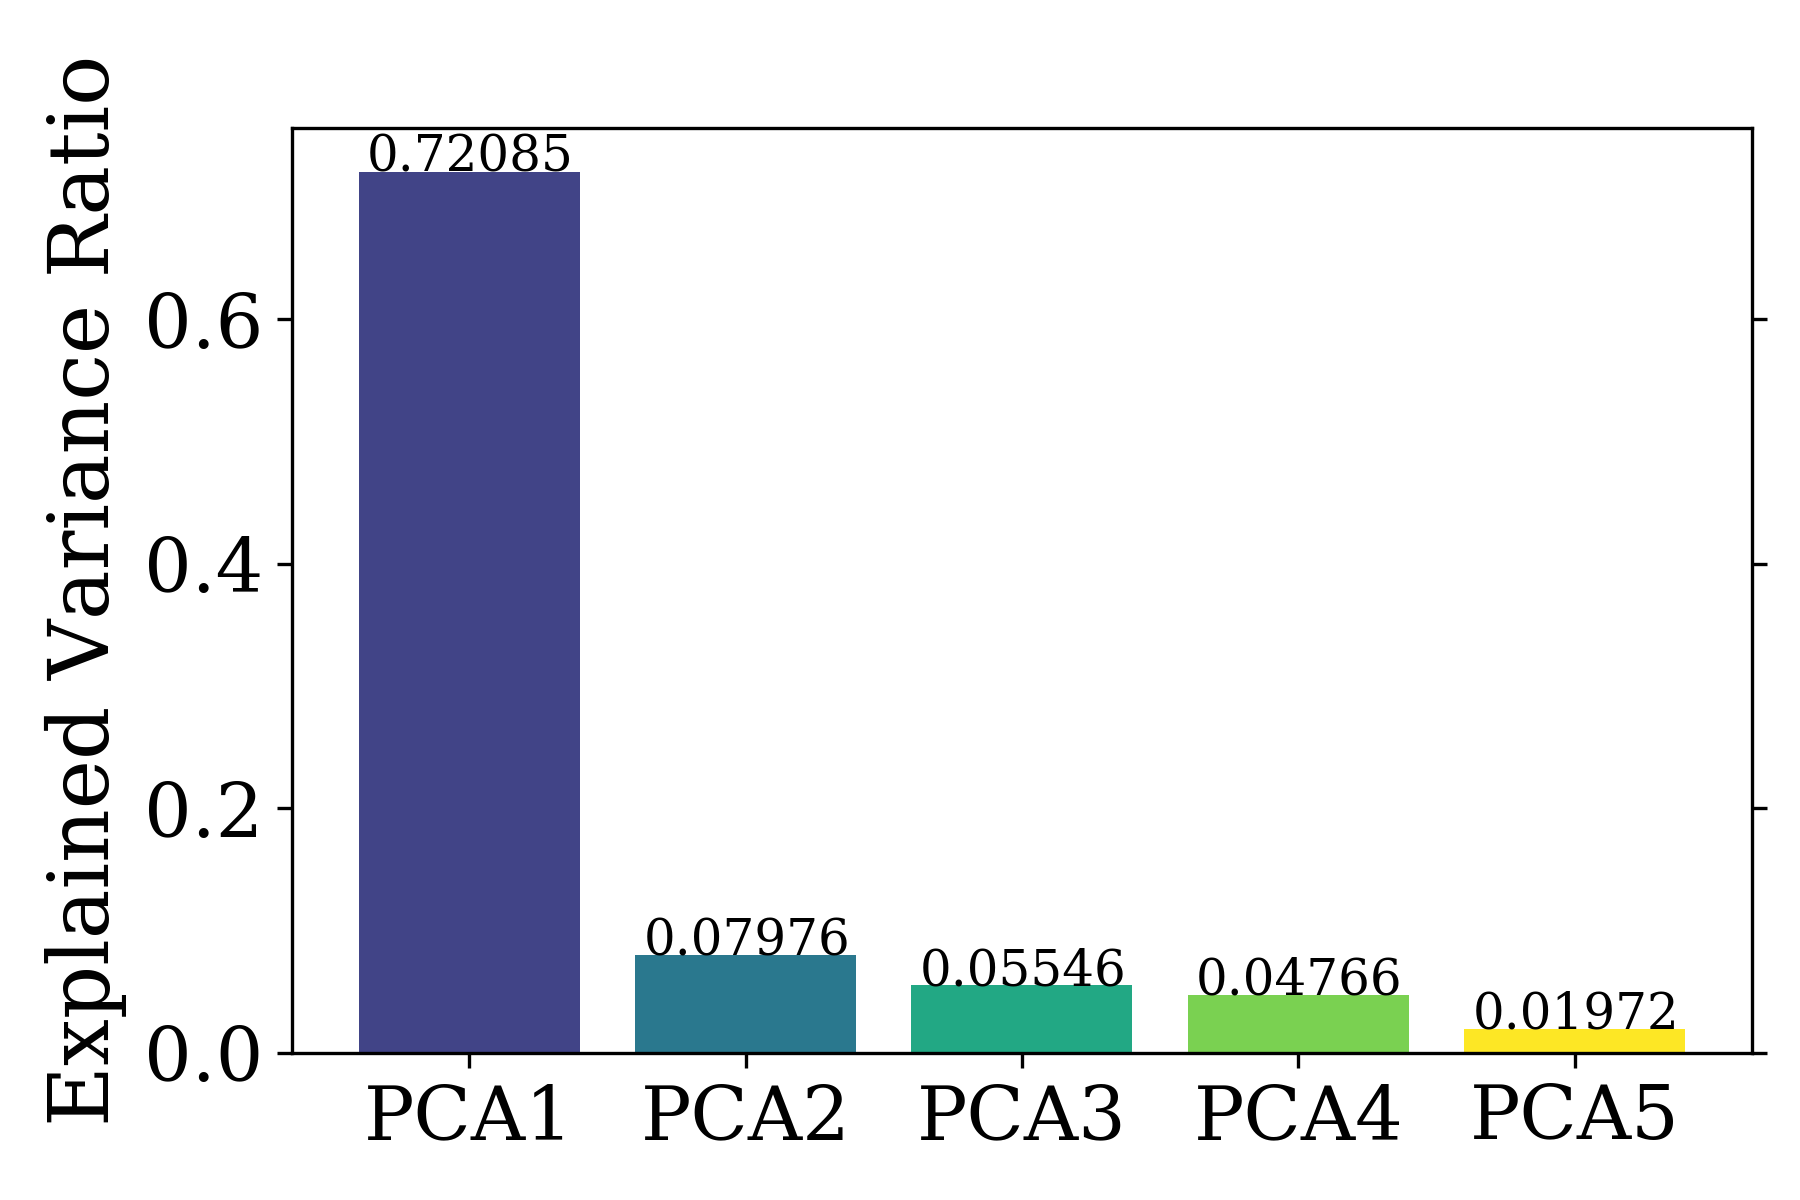
\includegraphics[scale=0.75]{supporting_images/FirstPCA.png}%scale=0.6
\caption{The First 5 Principle Dimensions v. Explained Variance Ratio}
\label{fig:FirstPCA}
\end{figure}

\par
Another way to group the data is with clustering. The clustering that was performed used a Gaussian Mixture clustering algorithm with two clusters on the first two principle axes of our PCA analysis. This is then plotted with a regular scale (figure \ref{fig:FirstCluster}), then a symmetric logarithmic scale (figure \ref{fig:SecondCluster}). This clustering achieved a silhouette score (see section \ref{Sil_score}) of 0.54681.

\begin{figure}[H]
\centering
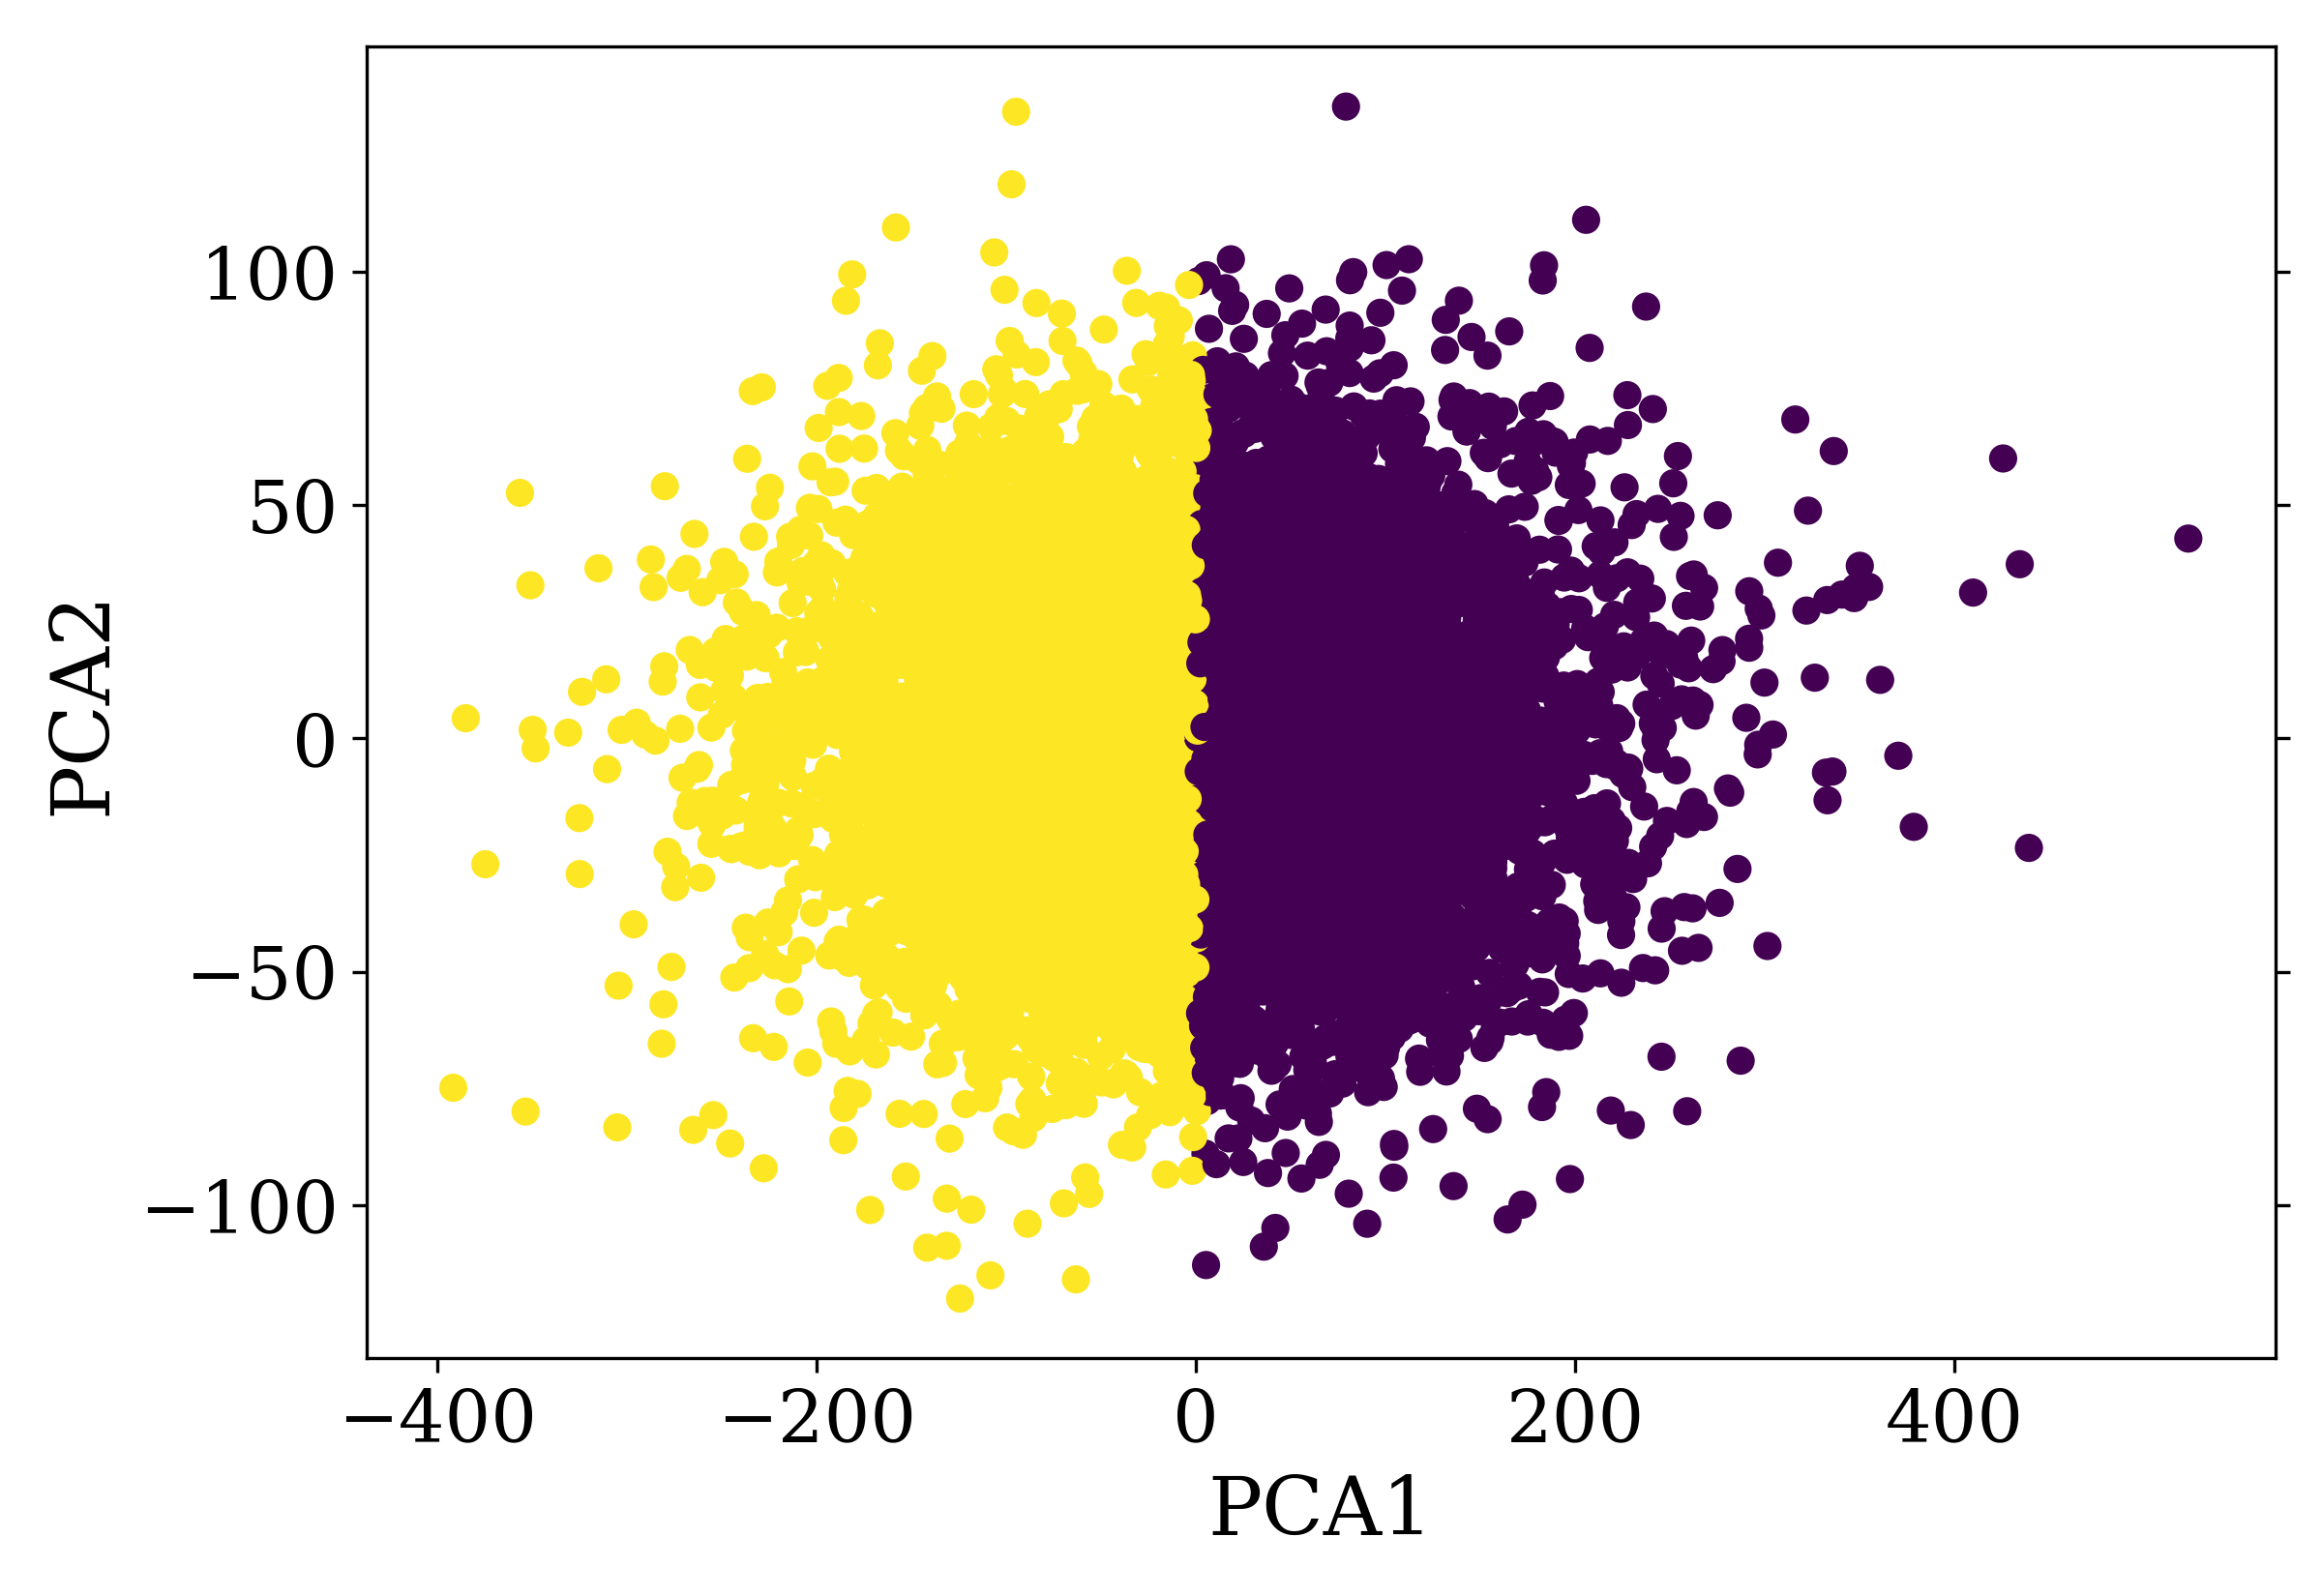
\includegraphics[scale=0.59]{supporting_images/FirstCluster.png}%scale=0.475
\caption{Second Principle Dimension v. First Principle Dimension with Clustering}
\label{fig:FirstCluster}
\end{figure}

\begin{figure}[H]
\centering
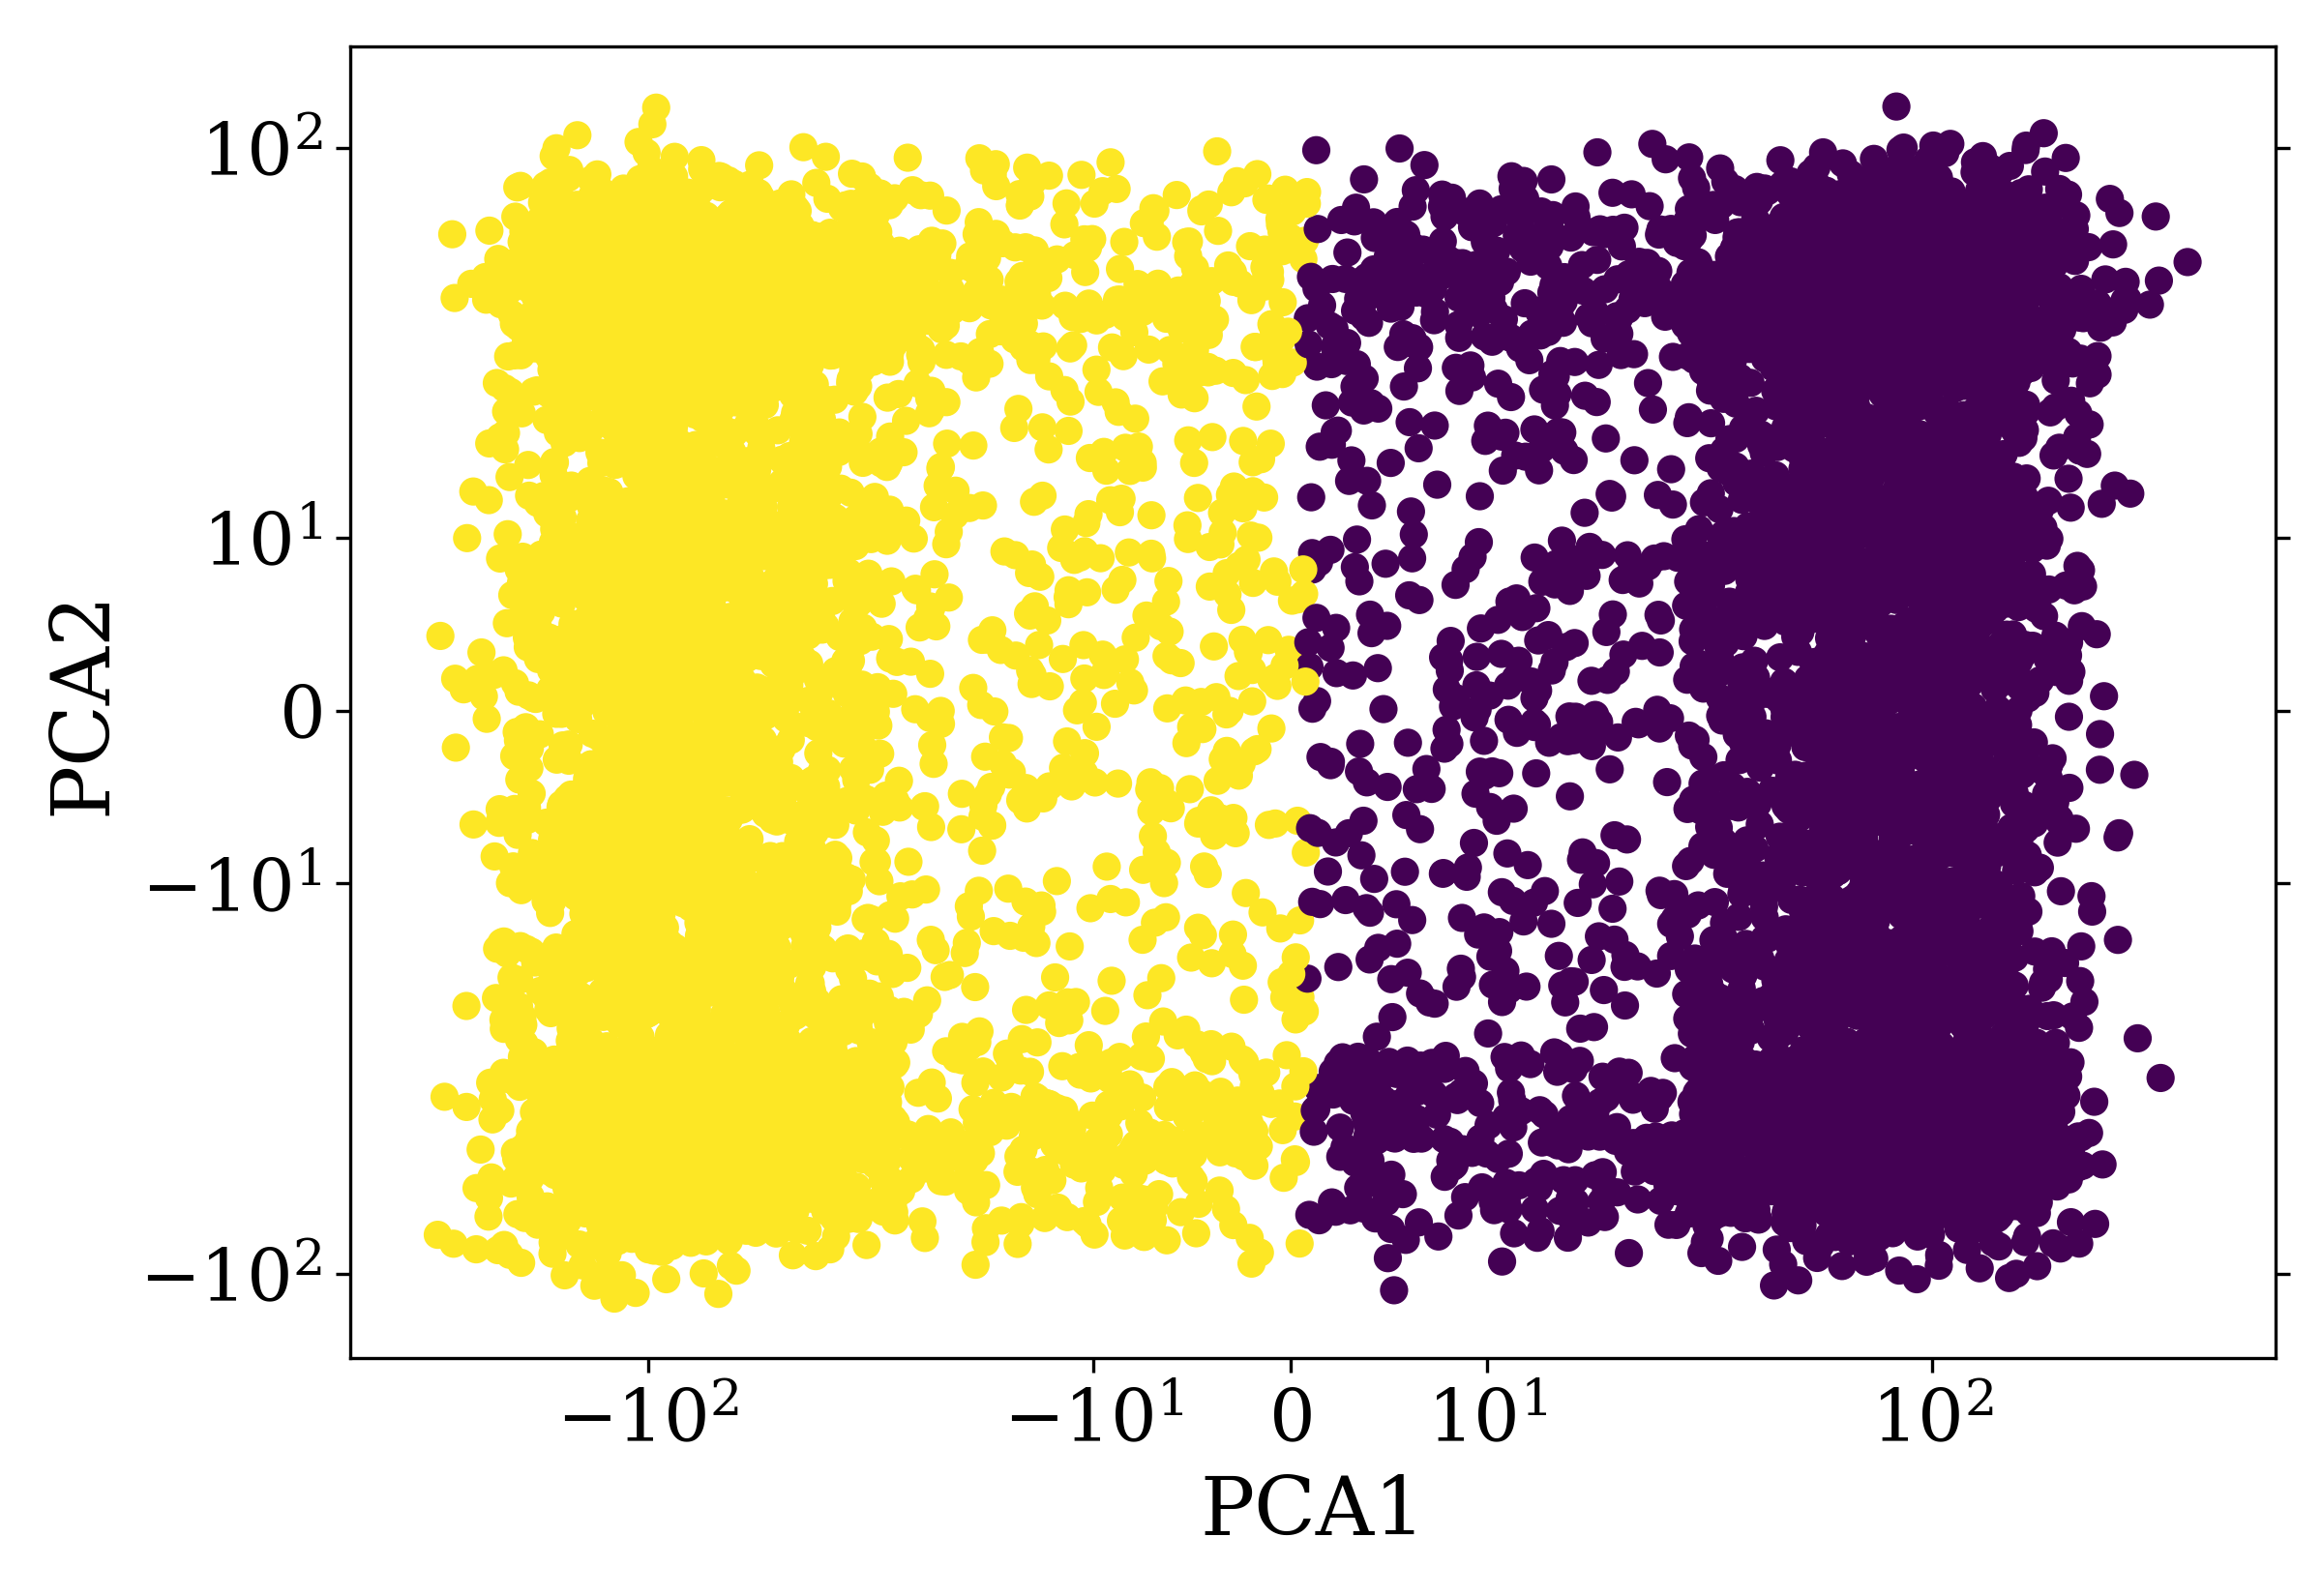
\includegraphics[scale=0.59]{supporting_images/SecondCluster.png}%scale=0.475
\caption{Second Principle Dimension v. First Principle Dimension with Clustering on a Symmetric Logarithmic Scale}
\label{fig:SecondCluster}
\end{figure}

\subsection{Algorithm Selection} \label{algorithm_selection}
\par
For this project, five different algorithms were analyzed to see which one would be the best for this application. The five algorithms are XGBoost Classifier (XGB), Support Vector Classifier (SVC), Adaptive Boosting (AdaBoost) Classifier, Gaussian Naive Bayes (GaussianNB), and Logistic Regression. 

\subsubsection{Support Vector Classifier}
\par
The Support Vector Classifier is a classification algorithm based on a Support Vector Machine (SVM). In the case of this project, the SVM is classifying with a RBF kernel. The Radial Basis Function (RBF) kernel in a two dimensional spacial sense, the SVC draws a mountain above each point. From there, a series of weights are calculated based on the heights of the mountains at each point. From those weights, the mountains are multiplied by a scaler. After that, a line is used to divide the high points from the low points. The high and low points are the binary classification for the system. This method is easily extrapolated to higher dimensions, allowing for classification of high dimensional data sets.

\subsubsection{AdaBoost Classifier}
\par
The AdaBoost Classifier used in the project has Decision Tree Classifiers (DTC) as the trees. The AdaBoost Classifier uses multiple DTCs as weak learners. These learners do not learn much on their own. They become strong when the AdaBoost Classifier adds the weights of the DTCs together, effectively creating one strong learner from the ensemble of weak learners.
\par
The Decision Tree Classifiers divide the data into two groups. Then the next level is divided into two groups and so on for a specific number of levels. With a shallow number of levels, the DTC will not learn much. This is good for a boosting algorithm like AdaBoost, for many weak learners combined are often stronger than one strong learner. An example of a decision tree is below.

\begin{figure}[H]
    \centering
    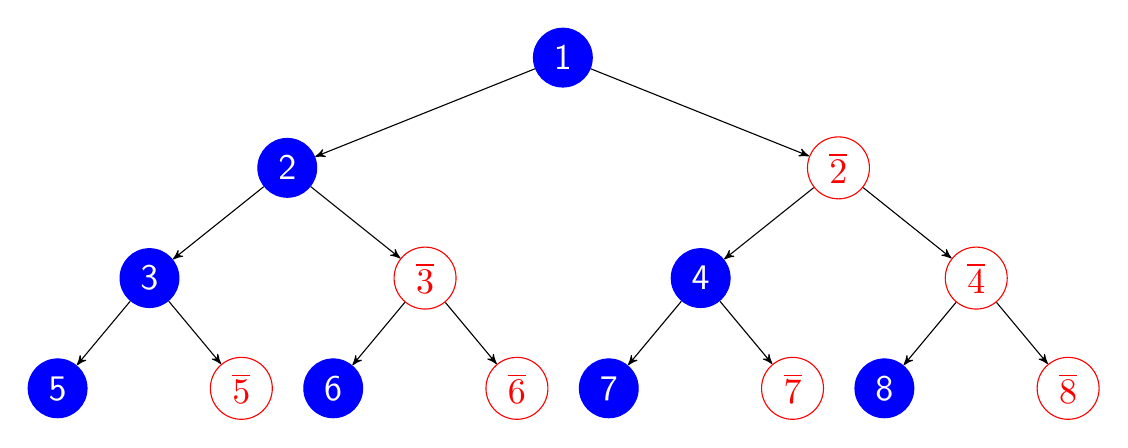
\begin{tikzpicture}[
        every node/.style={scale=1.3},
        ->,
        >=stealth',
        level/.style={sibling distance = 7cm/#1,
        level distance = 1.4cm}
    ]
    \node [top] {1}
        child{ node [top] {2}
            child{ node [top] {3}
                child{ node [top] {5}
                }
                child{ node [bottom] {$\overline{5}$}
                }
            }
            child{ node [bottom] {$\overline{3}$}
                child{ node [top] {6}
                }
                child{ node [bottom] {$\overline{6}$}
                }
            }
        }
        child{ node [bottom] {$\overline{2}$}
            child{ node [top] {4}
                child{ node [top] {7}
                }
                child{ node [bottom] {$\overline{7}$}
                }
            }
            child{ node [bottom] {$\overline{4}$}
                child{ node [top] {8}
                }
                child{ node [bottom] {$\overline{8}$}
                }
            }
        }
    ;
    \end{tikzpicture}
    \caption{Example Decision Tree Classifier Tree}
    \label{fig:tree}
\end{figure}

\subsubsection{XGBoost Classifier}
\par
The XGBoost Classifier is a gradient boosting algorithm, similar to AdaBoost, that is designed with optimization and distributed computing in mind. This comes very efficient memory use for large data sets. XGBoost uses Decision Tree Classifiers like AdaBoost. But the way XGBoost combines the weak learners is different from AdaBoost. XGBoost uses a technique call Newton Boosting which uses the Newton-Paphson method. The Newton-Paphson method uses a direct route to find local minima instead of using gradient decent.

\subsubsection{Gaussian Naive Bayes}
\par
The Gaussian Naive Bayes algorithm is a probabilistic classifier that relies on the naive assumption of independence among the features. The Gaussian Naive Bayes is based on Bayes Theorem. This theorem is stated by the following equation
$$P(A|B) = \frac{P(B|A)*P(A)}{P(B)}$$
This formula is used to take known data from the training set to then infer the probabilities of a new sample. This is a very simple, but effective way to classify a data set.

\subsubsection{Logistic Regression}
\par
Logistic Regression is simply a linear regression, but used for binary classification. In a two dimensional sense, anything above the line would be classified as one group, everything below the line would be classified as the other group. This is extrapolated to higher dimensions and is a fairly simple model.

\subsubsection{Selection Results}
\par
In selecting an algorithm, each was tested with both the transformed data from the data set and the PCA analysis in section \ref{PCA}. Both data sets were separated into training and testing groups, with approximately 15\% of the data in the testing set. Both data sets were preprocessed by scaling each dimension to a range to [-1, 1]. Accuracy of the training set, accuracy of the testing set, F1 score, precision, and training time were all recorded. The results are in the figures below. %Do I need documentation for these algorithms?

%Training Set Accuracy
\begin{figure}[H]
    \centering
    \begin{subfigure}[t]{0.495\textwidth}
        \centering
        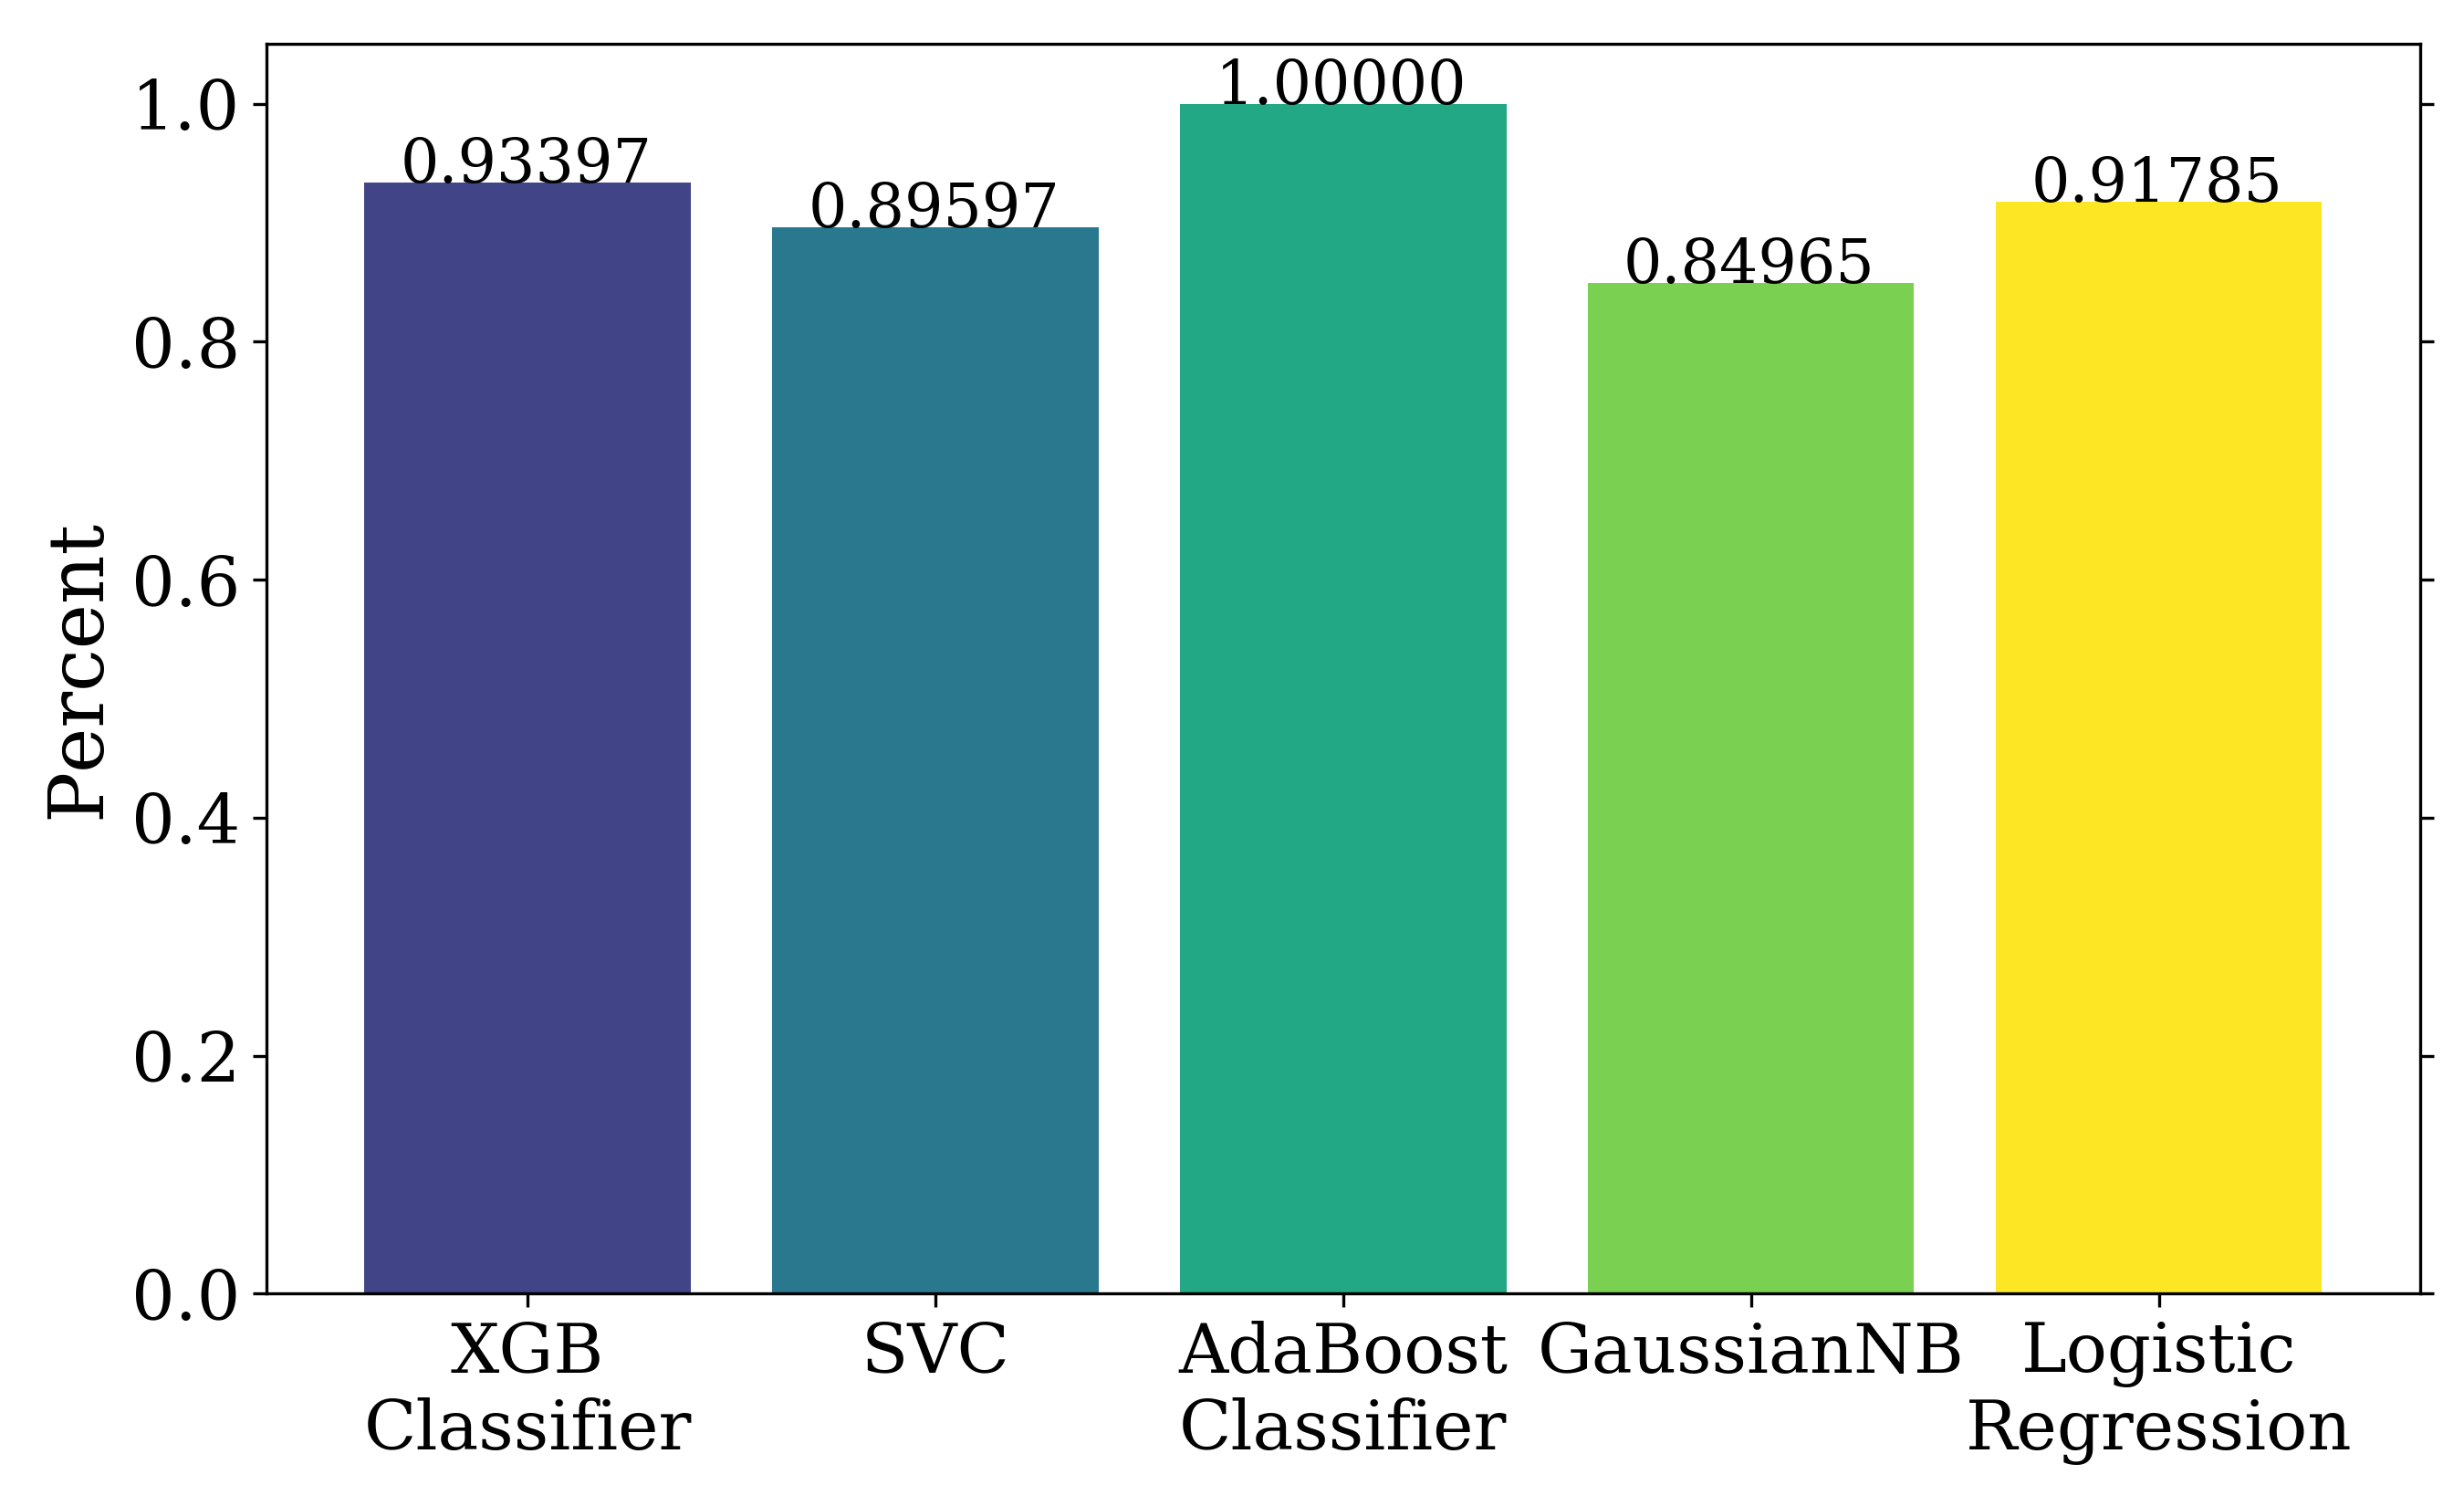
\includegraphics[width=\textwidth]{supporting_images/train_acc_notpca.png}
        \caption{Fitted with the whole data set}
        \label{fig:train_acc_notpca}
    \end{subfigure}
    \hfill
    \begin{subfigure}[t]{0.495\textwidth}
        \centering
        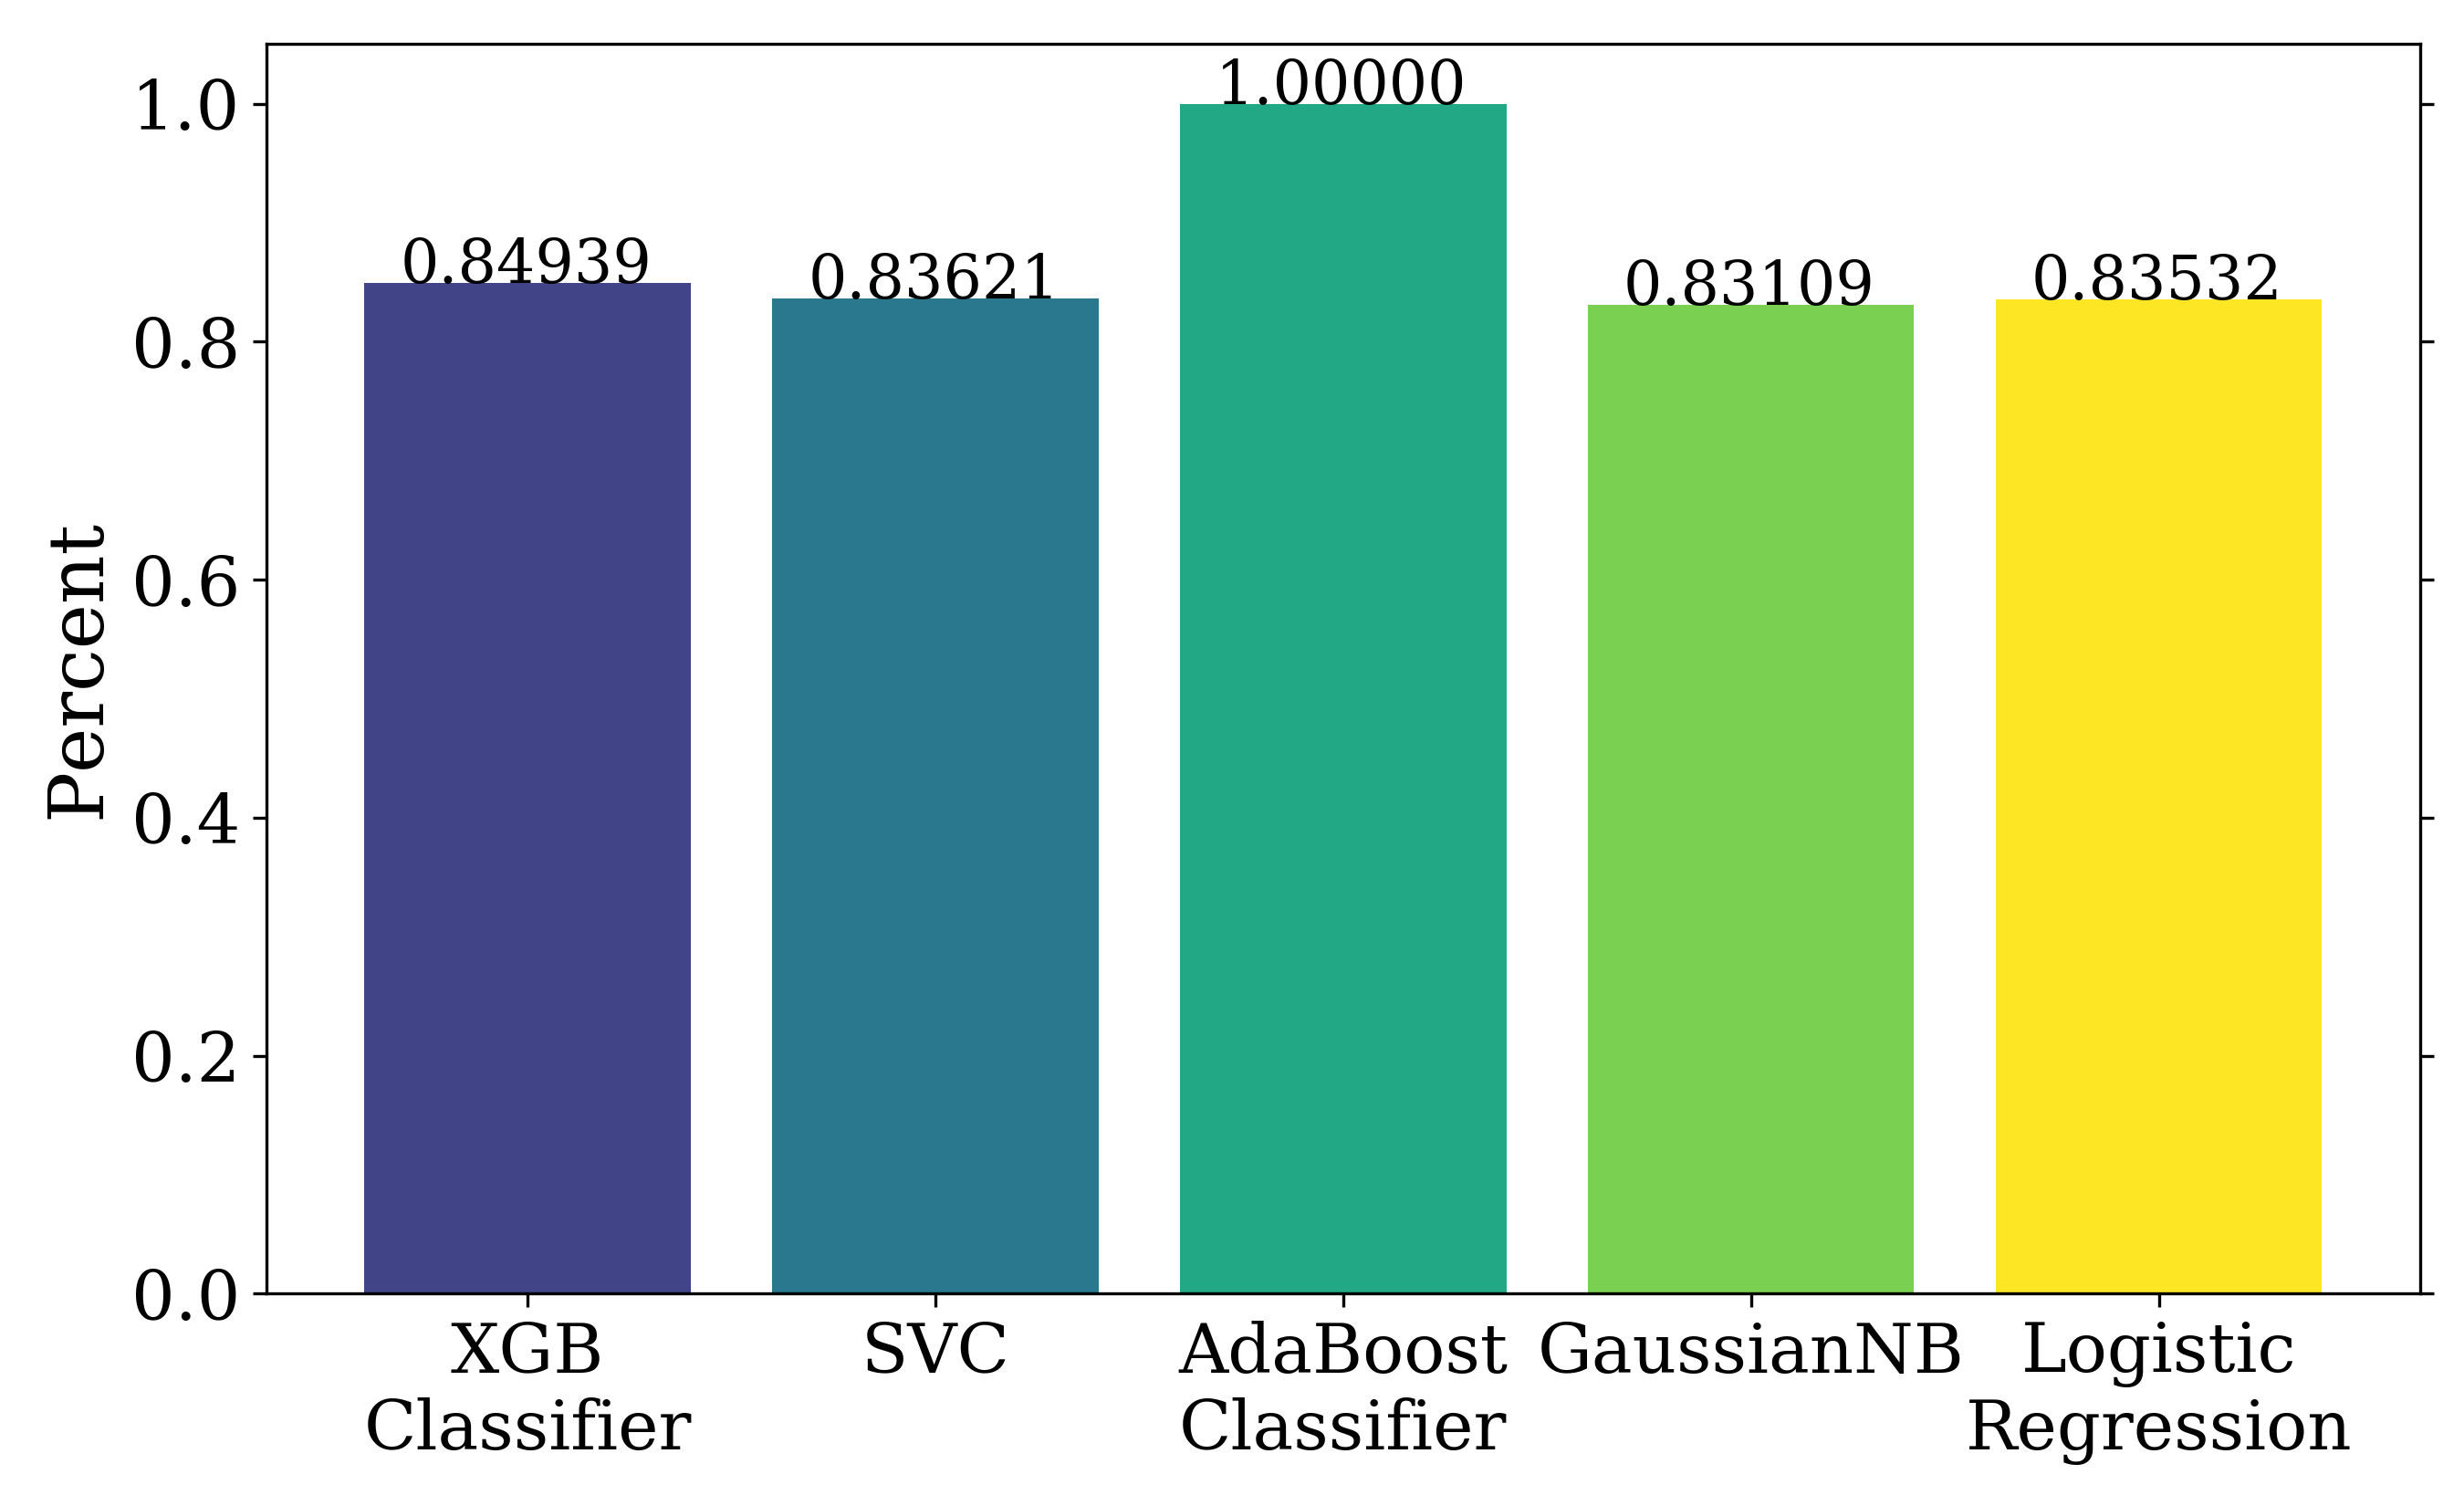
\includegraphics[width=\textwidth]{supporting_images/train_acc_pca.png}
        \caption{Fitted with the transformed PCA data set}
        \label{fig:train_acc_pca}
    \end{subfigure}
    \caption{Training Set Accuracy}
    \label{fig:train_acc}
\end{figure}

%Testing Set Accuracy
\begin{figure}[H]
    \centering
    \begin{subfigure}[t]{0.495\textwidth}
        \centering
        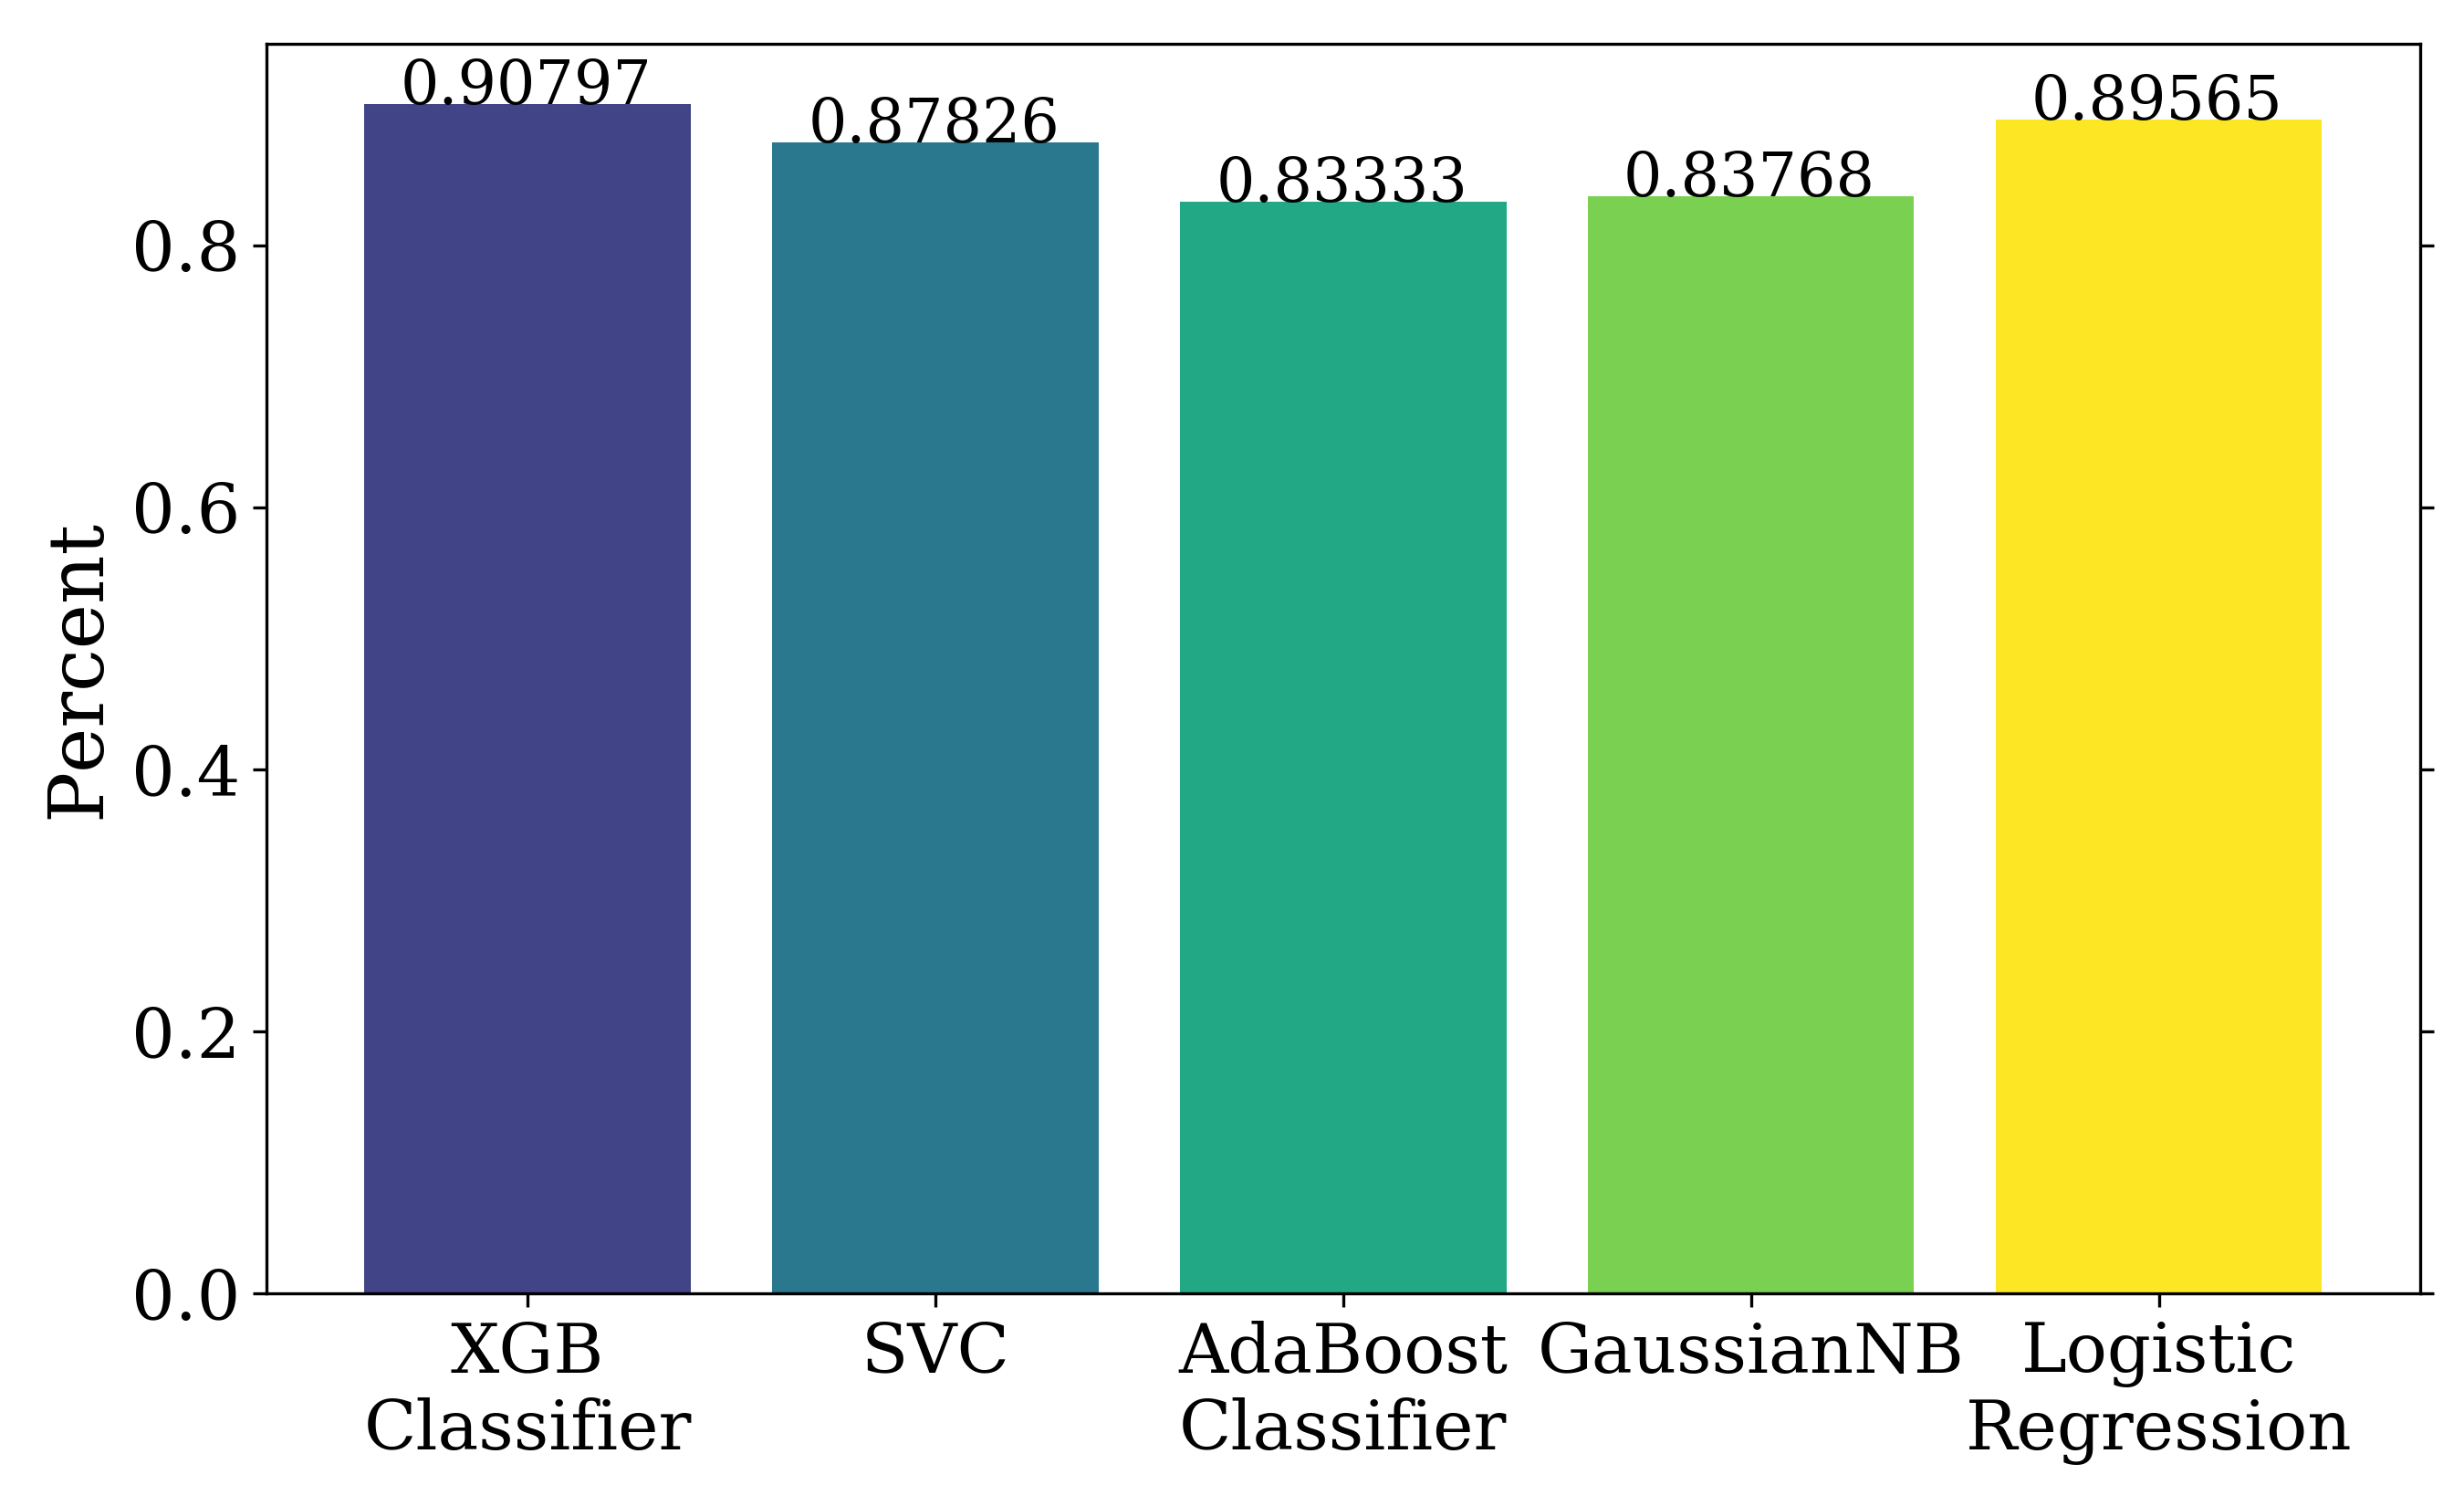
\includegraphics[width=\textwidth]{supporting_images/test_acc_notpca.png}
        \caption{Fitted with the whole data set}
        \label{fig:test_acc_notpca}
    \end{subfigure}
    \hfill
    \begin{subfigure}[t]{0.495\textwidth}
        \centering
        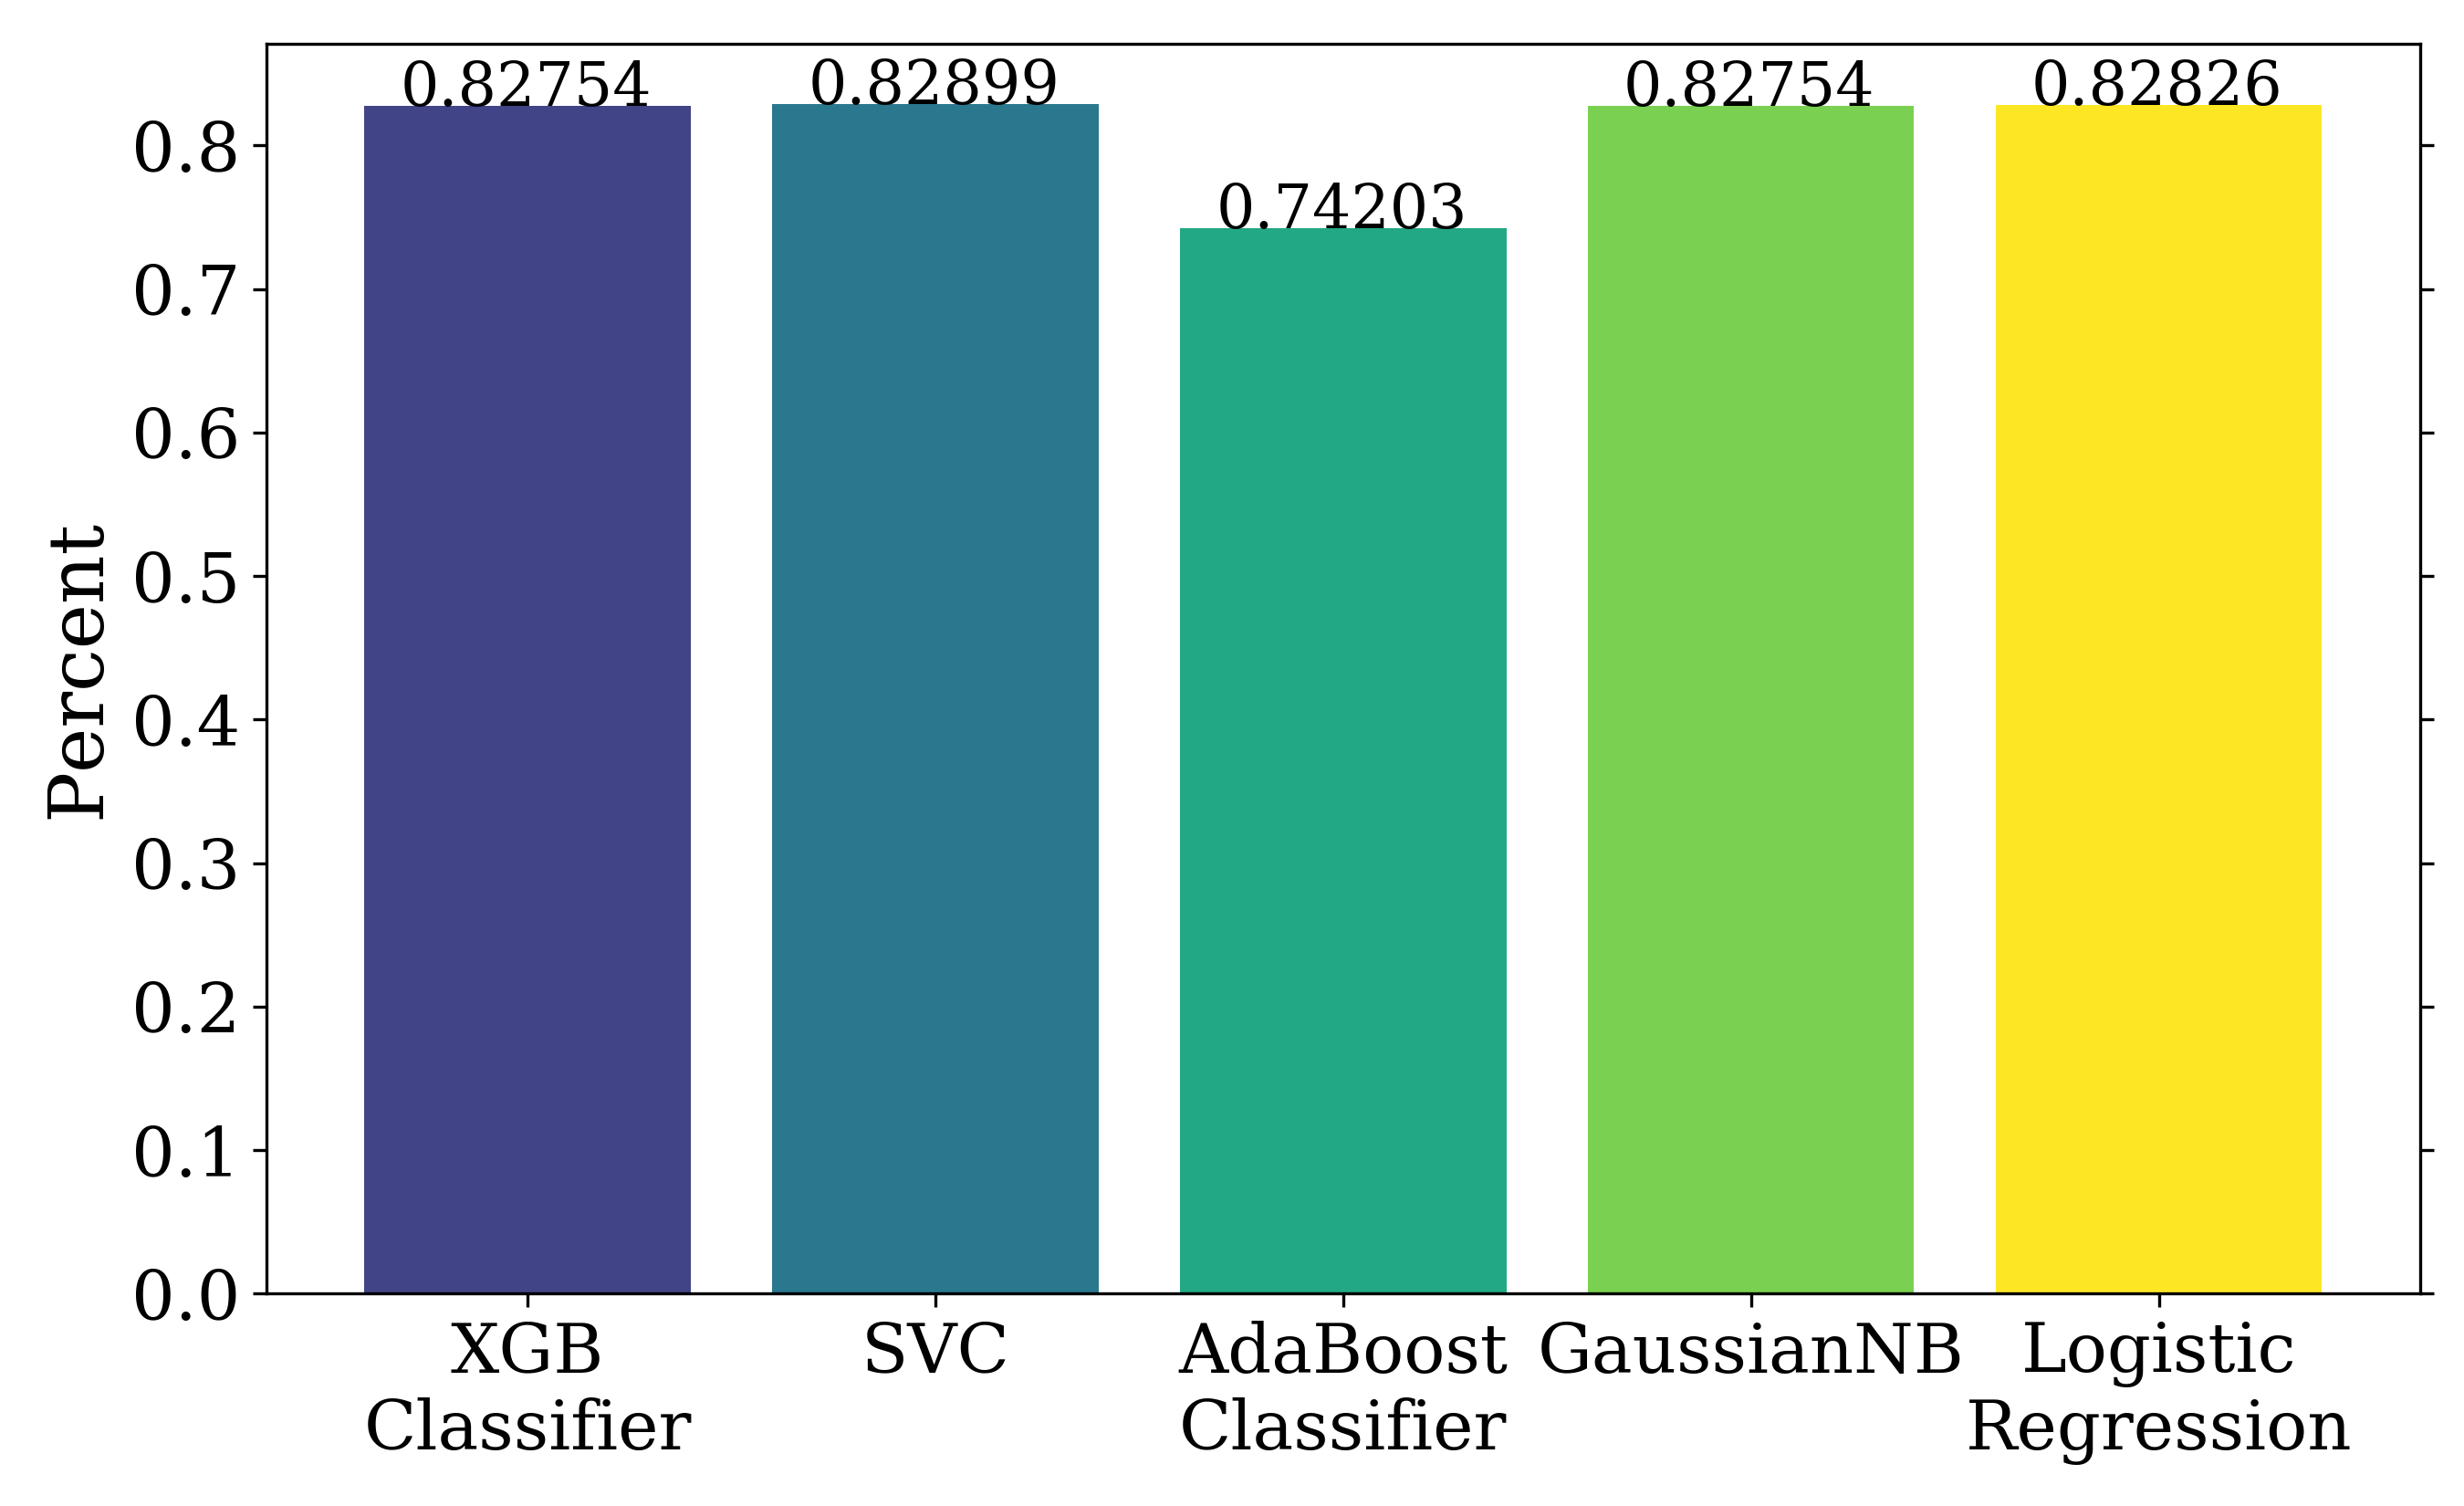
\includegraphics[width=\textwidth]{supporting_images/test_acc_pca.png}
        \caption{Fitted with the transformed PCA data set}
        \label{fig:test_acc_pca}
    \end{subfigure}
    \caption{Testing Set Accuracy}
    \label{fig:test_acc}
\end{figure}

%F1 Score
\begin{figure}[H]
    \centering
    \begin{subfigure}[t]{0.495\textwidth}
        \centering
        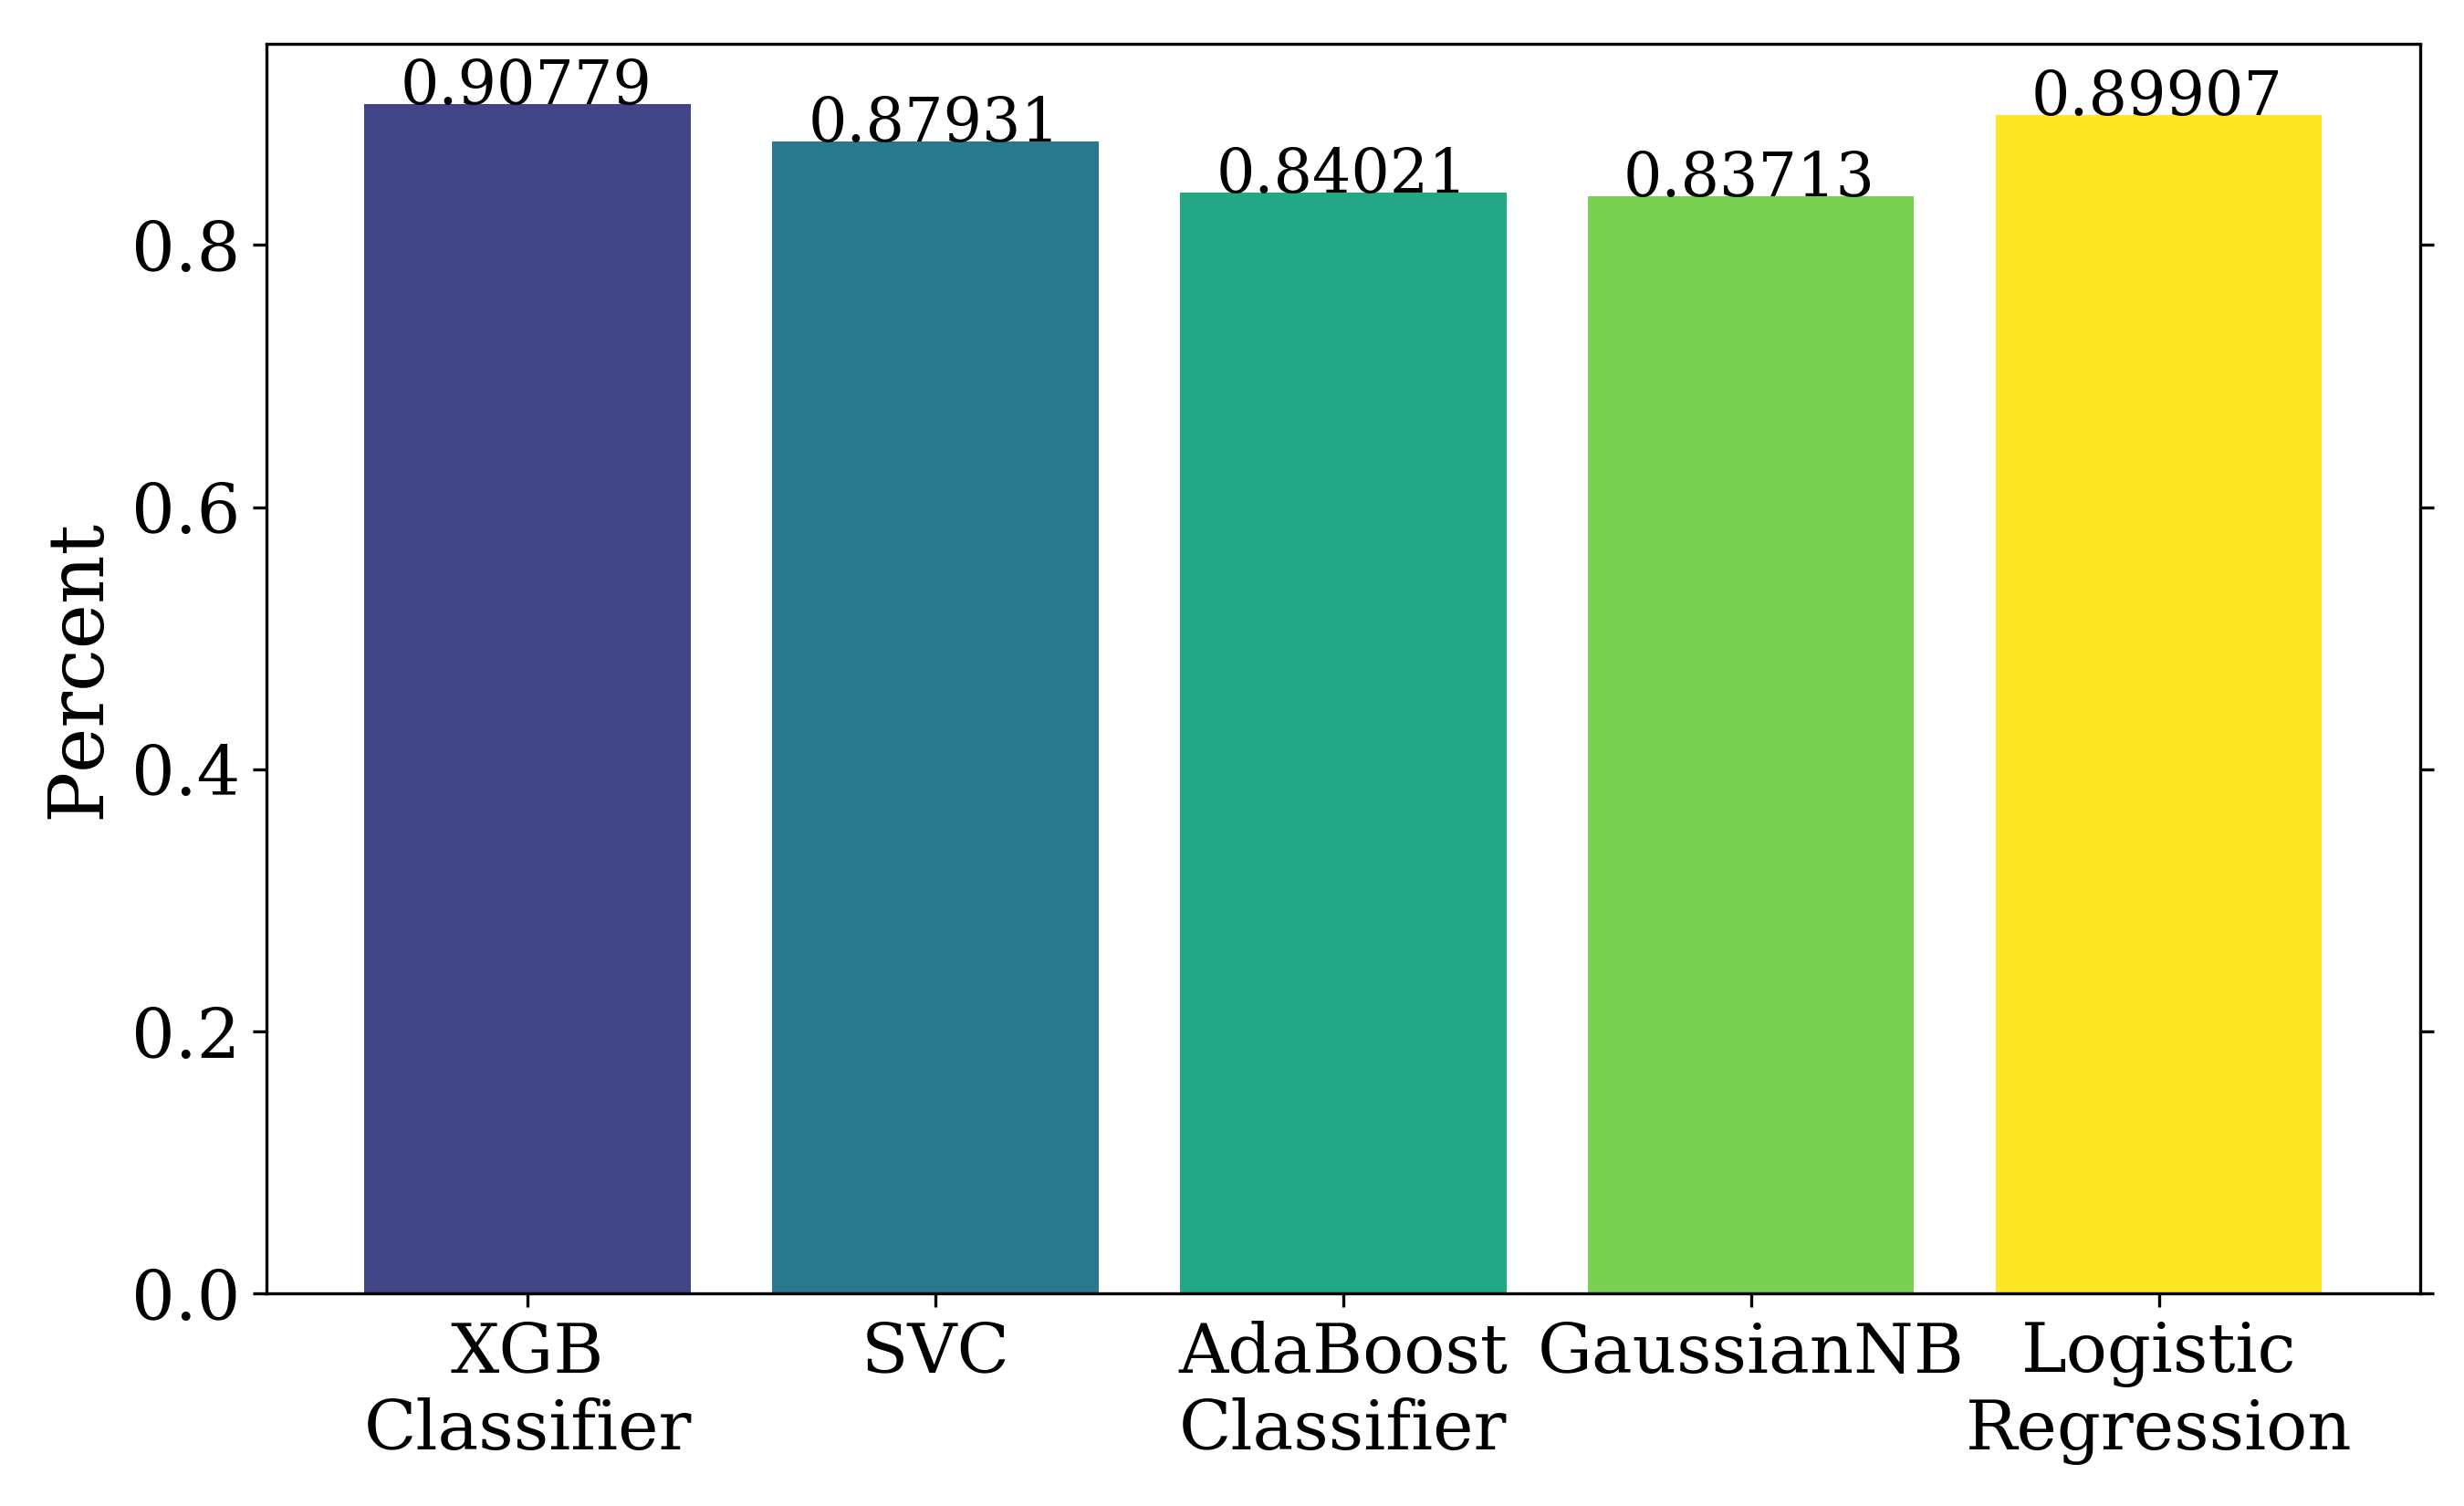
\includegraphics[width=\textwidth]{supporting_images/fbeta_notpca.png}
        \caption{Fitted with the whole data set}
        \label{fig:fbeta_notpca}
    \end{subfigure}
    \hfill
    \begin{subfigure}[t]{0.495\textwidth}
        \centering
        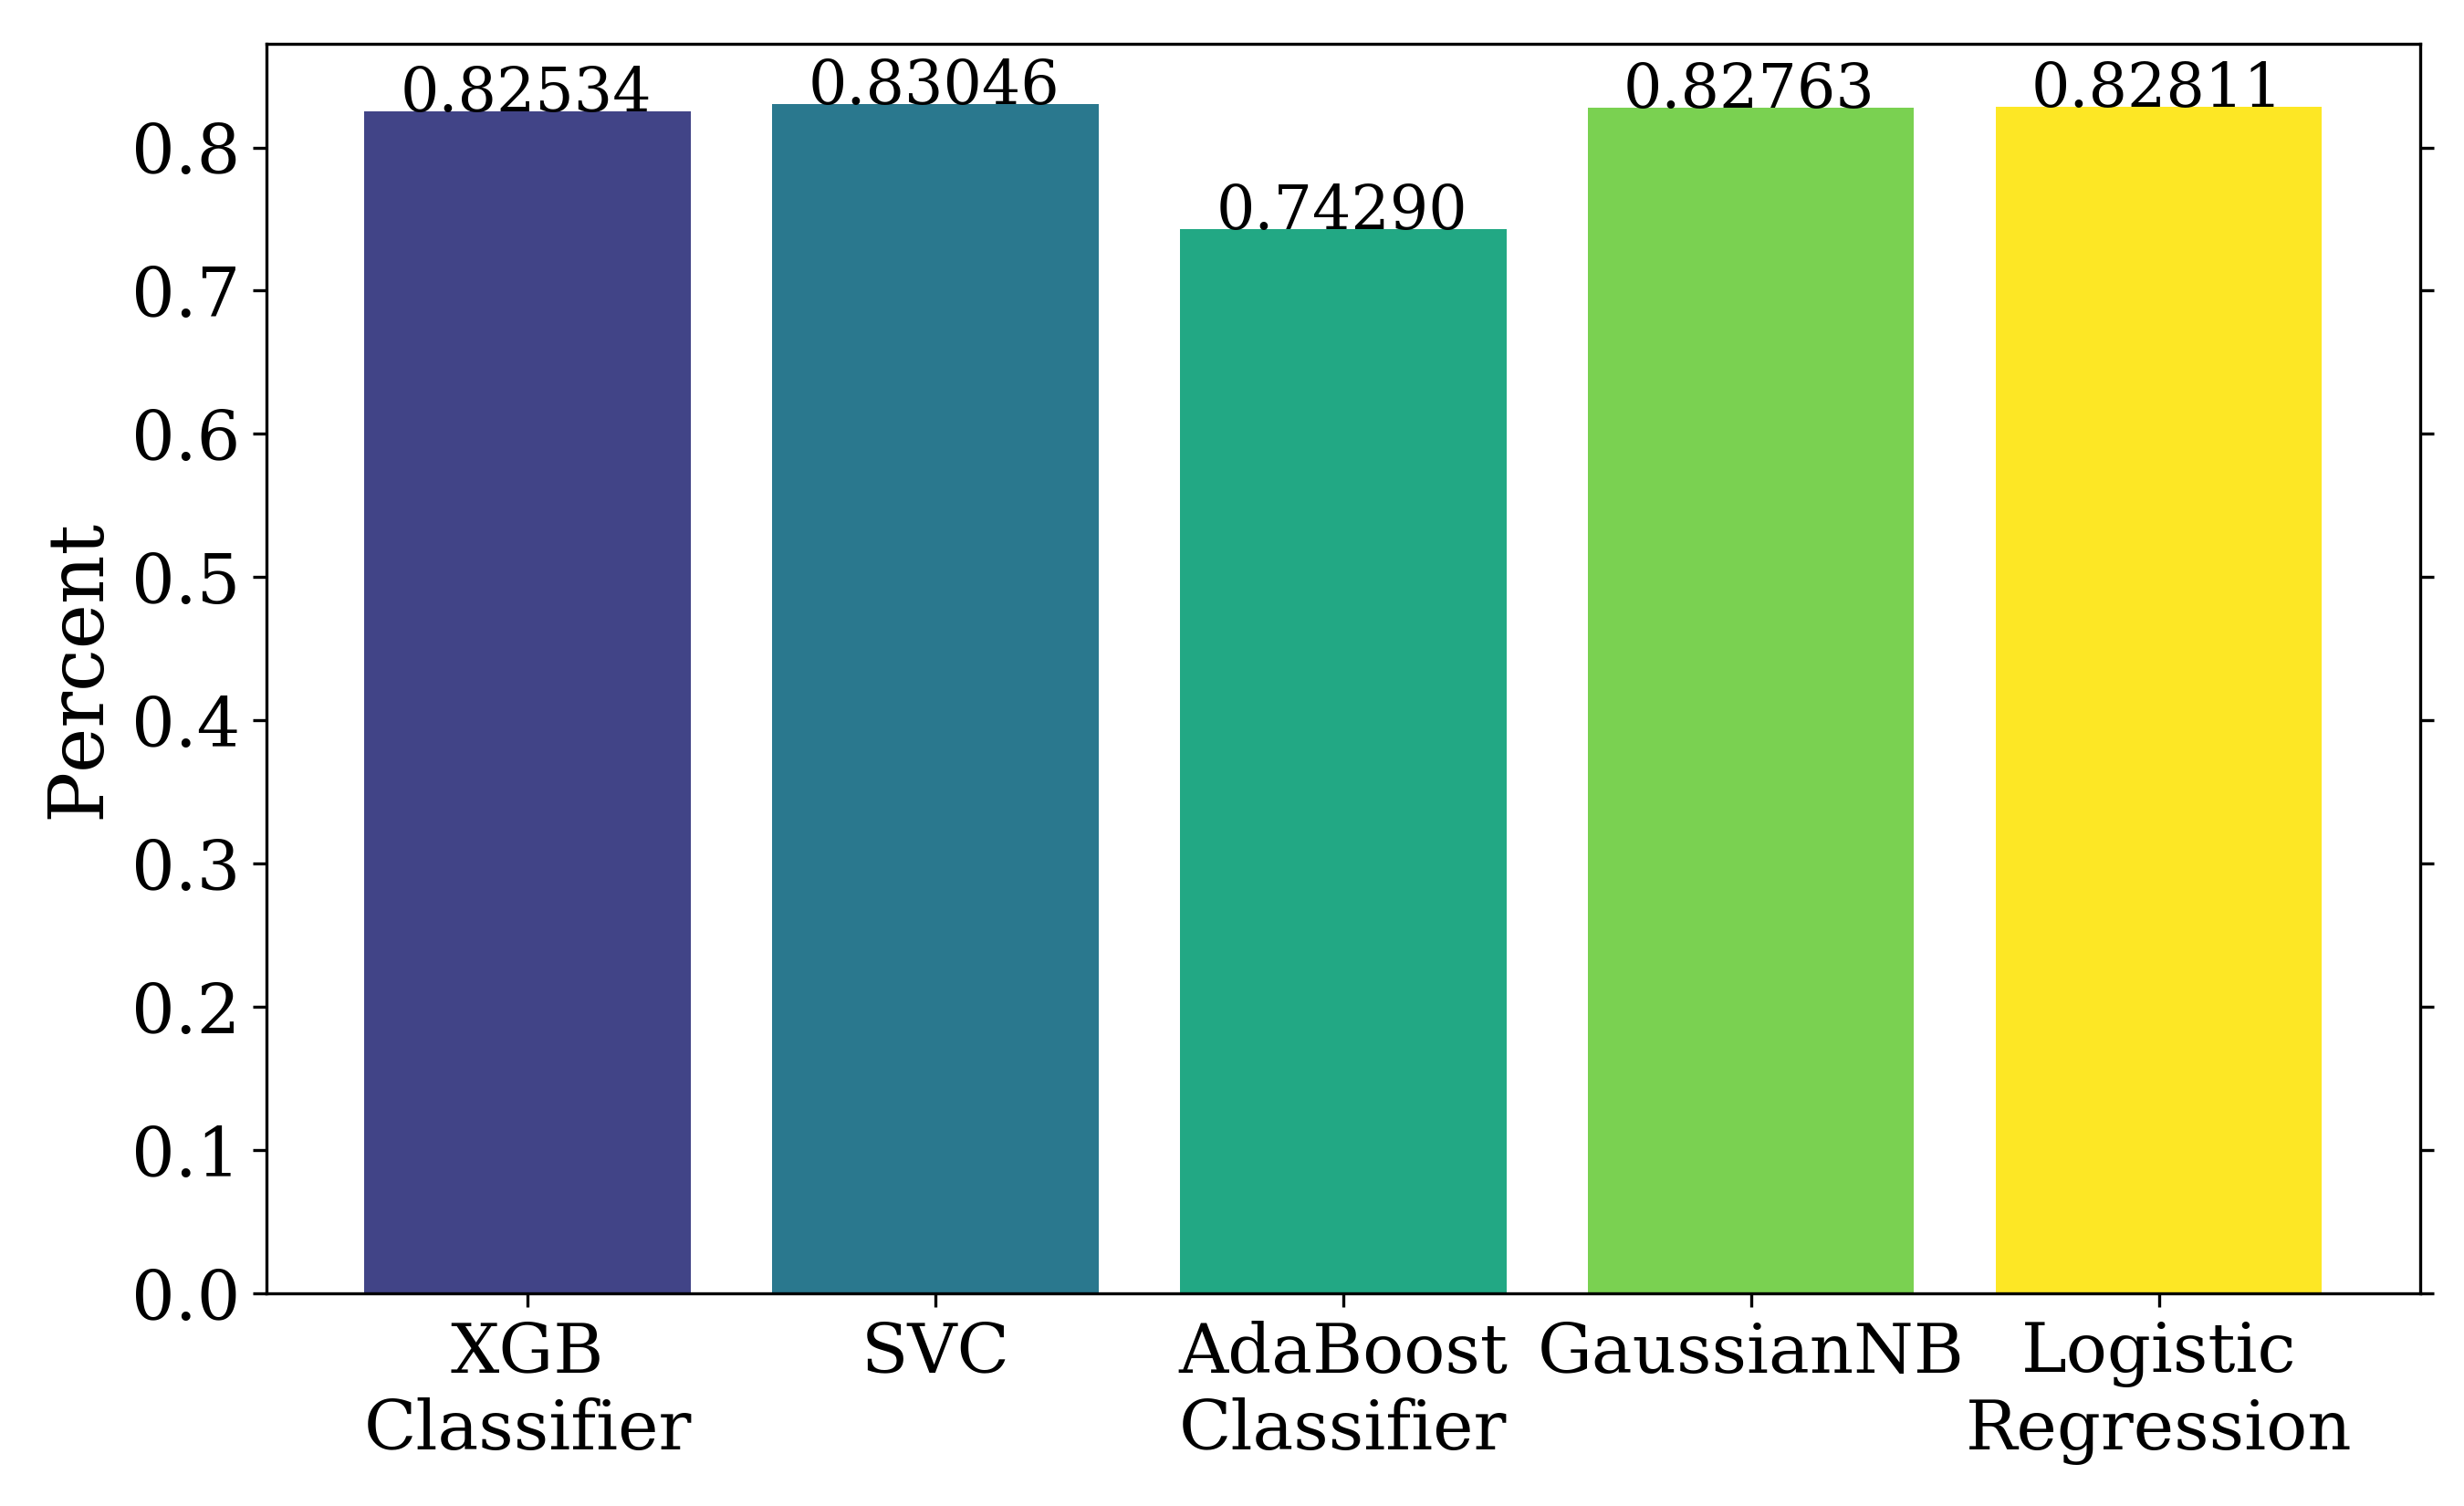
\includegraphics[width=\textwidth]{supporting_images/fbeta_pca.png}
        \caption{Fitted with the transformed PCA data set}
        \label{fig:fbeta_pca}
    \end{subfigure}
    \caption{F1 Score}
    \label{fig:fbeta}
\end{figure}

%Precision Score
\begin{figure}[H]
    \centering
    \begin{subfigure}[t]{0.495\textwidth}
        \centering
        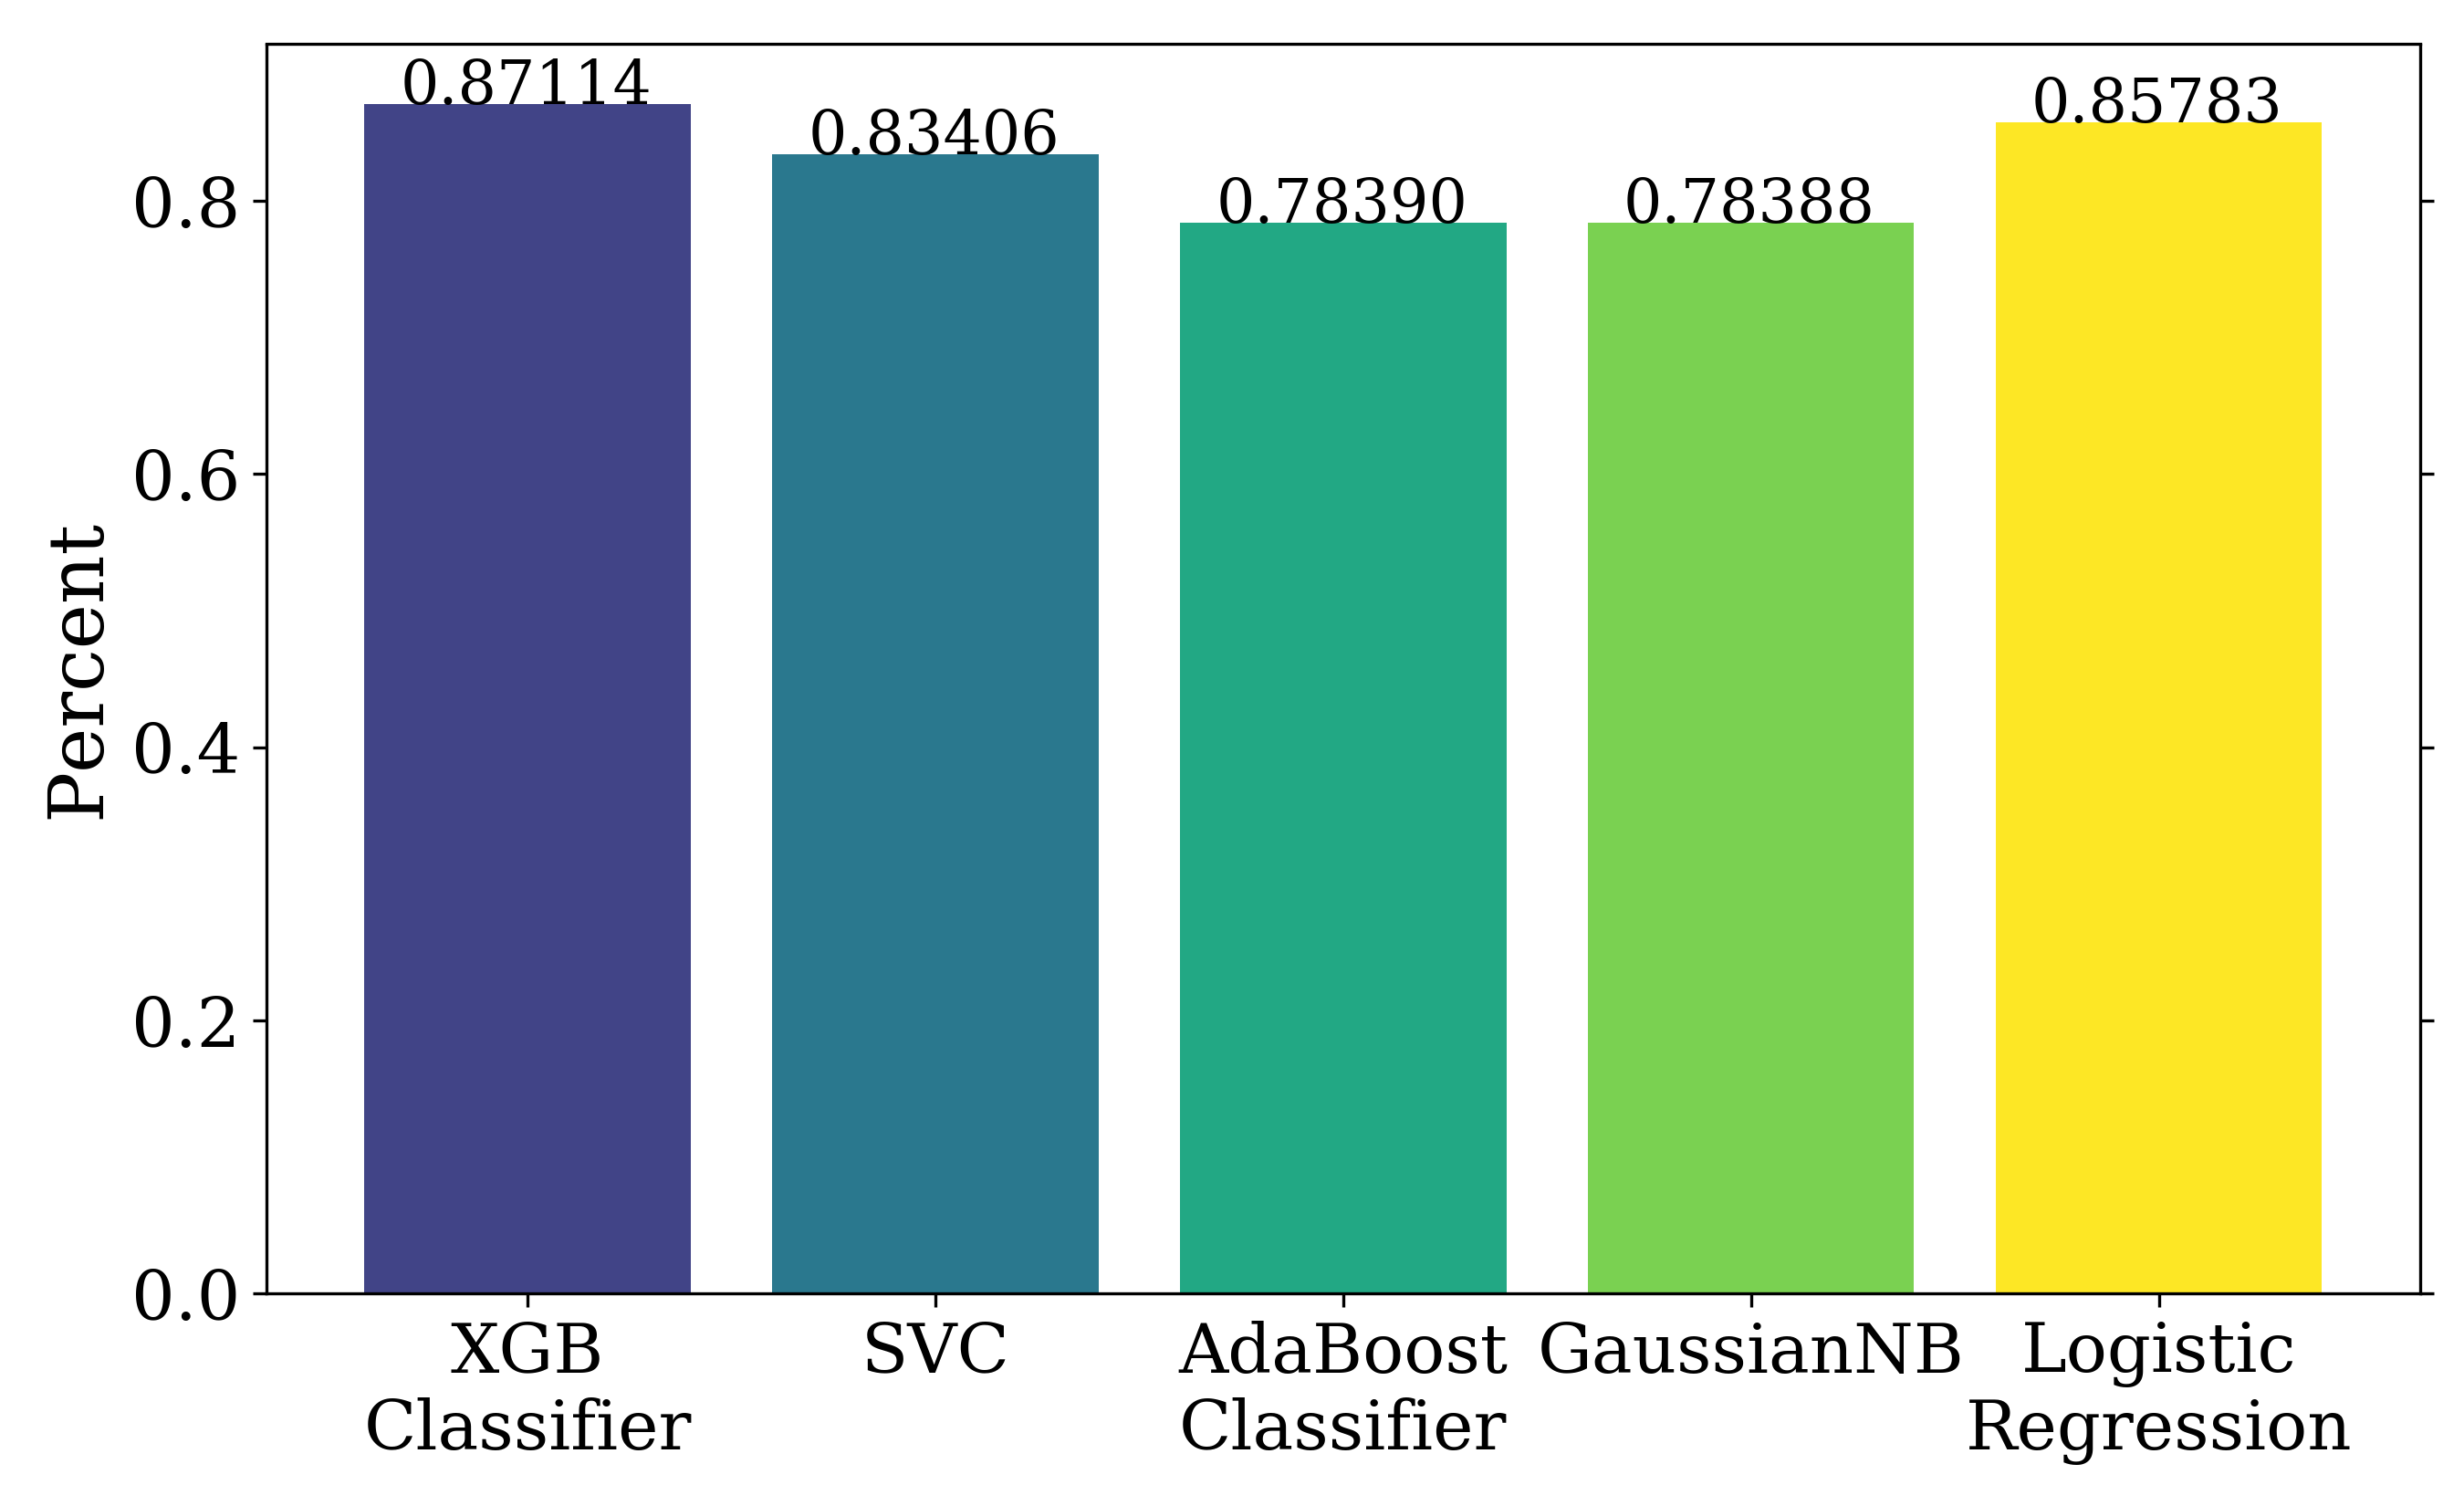
\includegraphics[width=\textwidth]{supporting_images/precision_notpca.png}
        \caption{Fitted with the whole data set}
        \label{fig:precision_notpca}
    \end{subfigure}
    \hfill
    \begin{subfigure}[t]{0.495\textwidth}
        \centering
        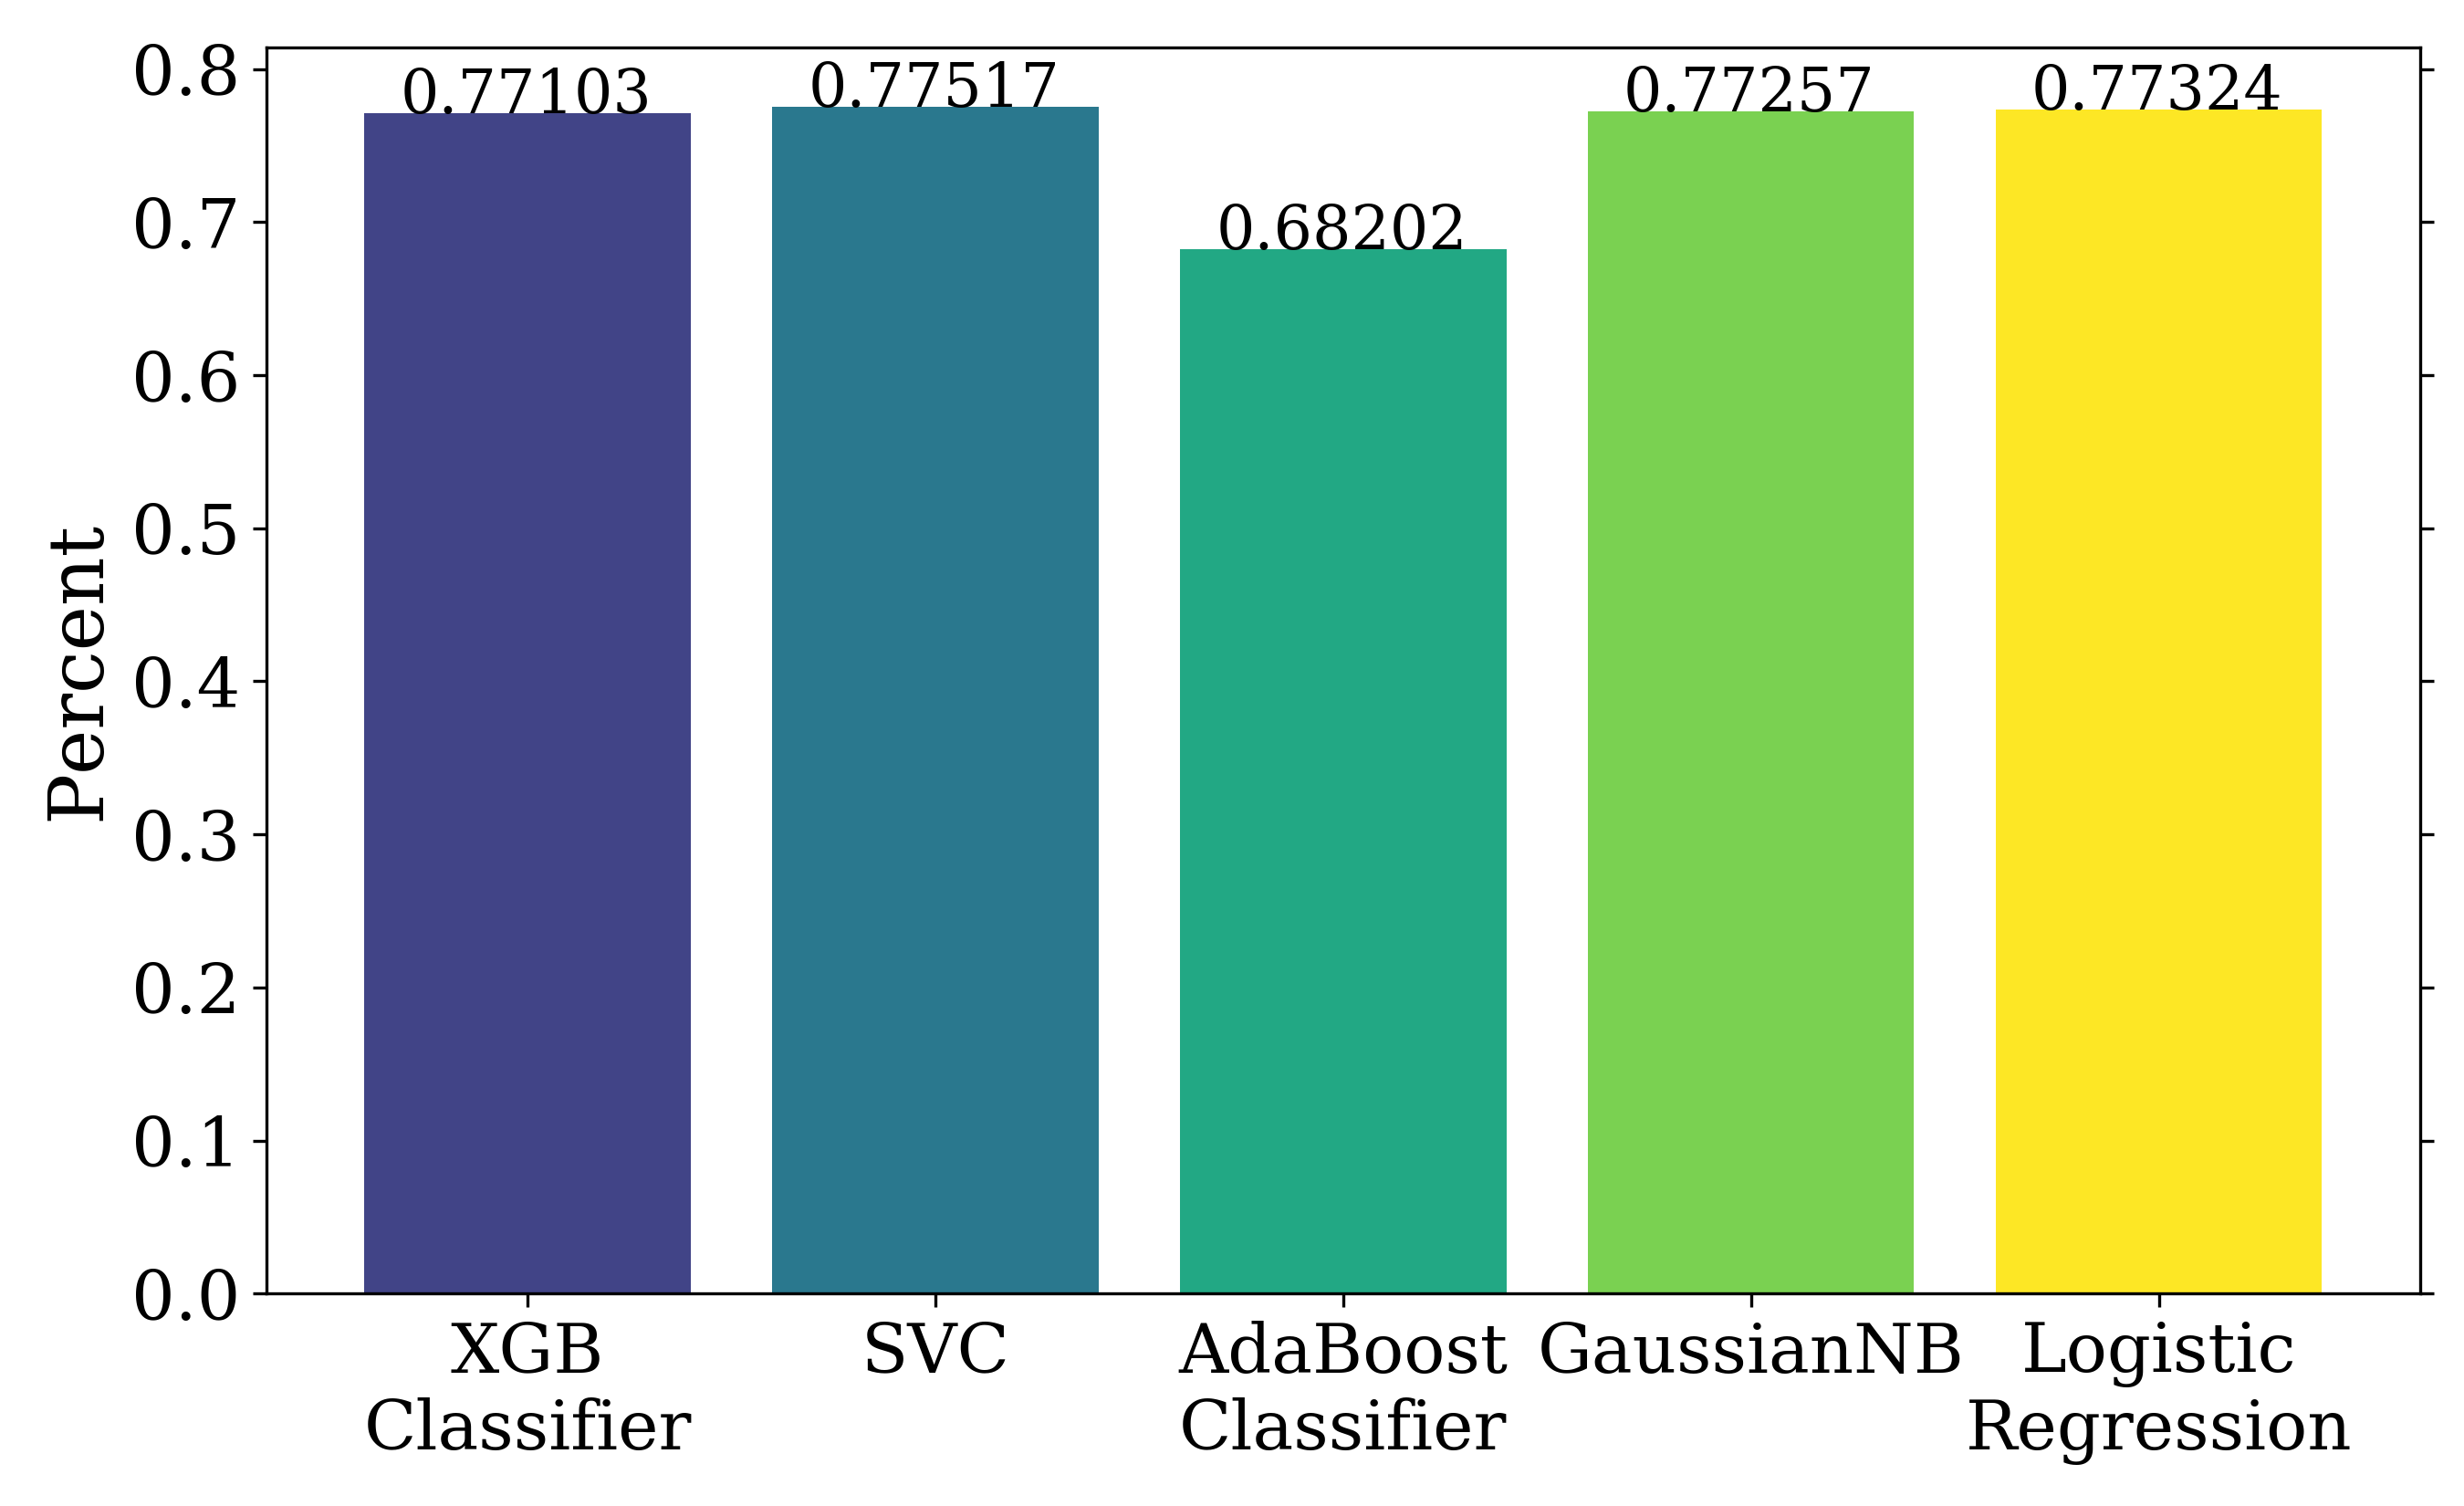
\includegraphics[width=\textwidth]{supporting_images/precision_pca.png}
        \caption{Fitted with the transformed PCA data set}
        \label{fig:precision_pca}
    \end{subfigure}
    \caption{Precision Score}
    \label{fig:precision}
\end{figure}

%Training Time
\begin{figure}[H]
    \centering
    \begin{subfigure}[t]{0.495\textwidth}
        \centering
        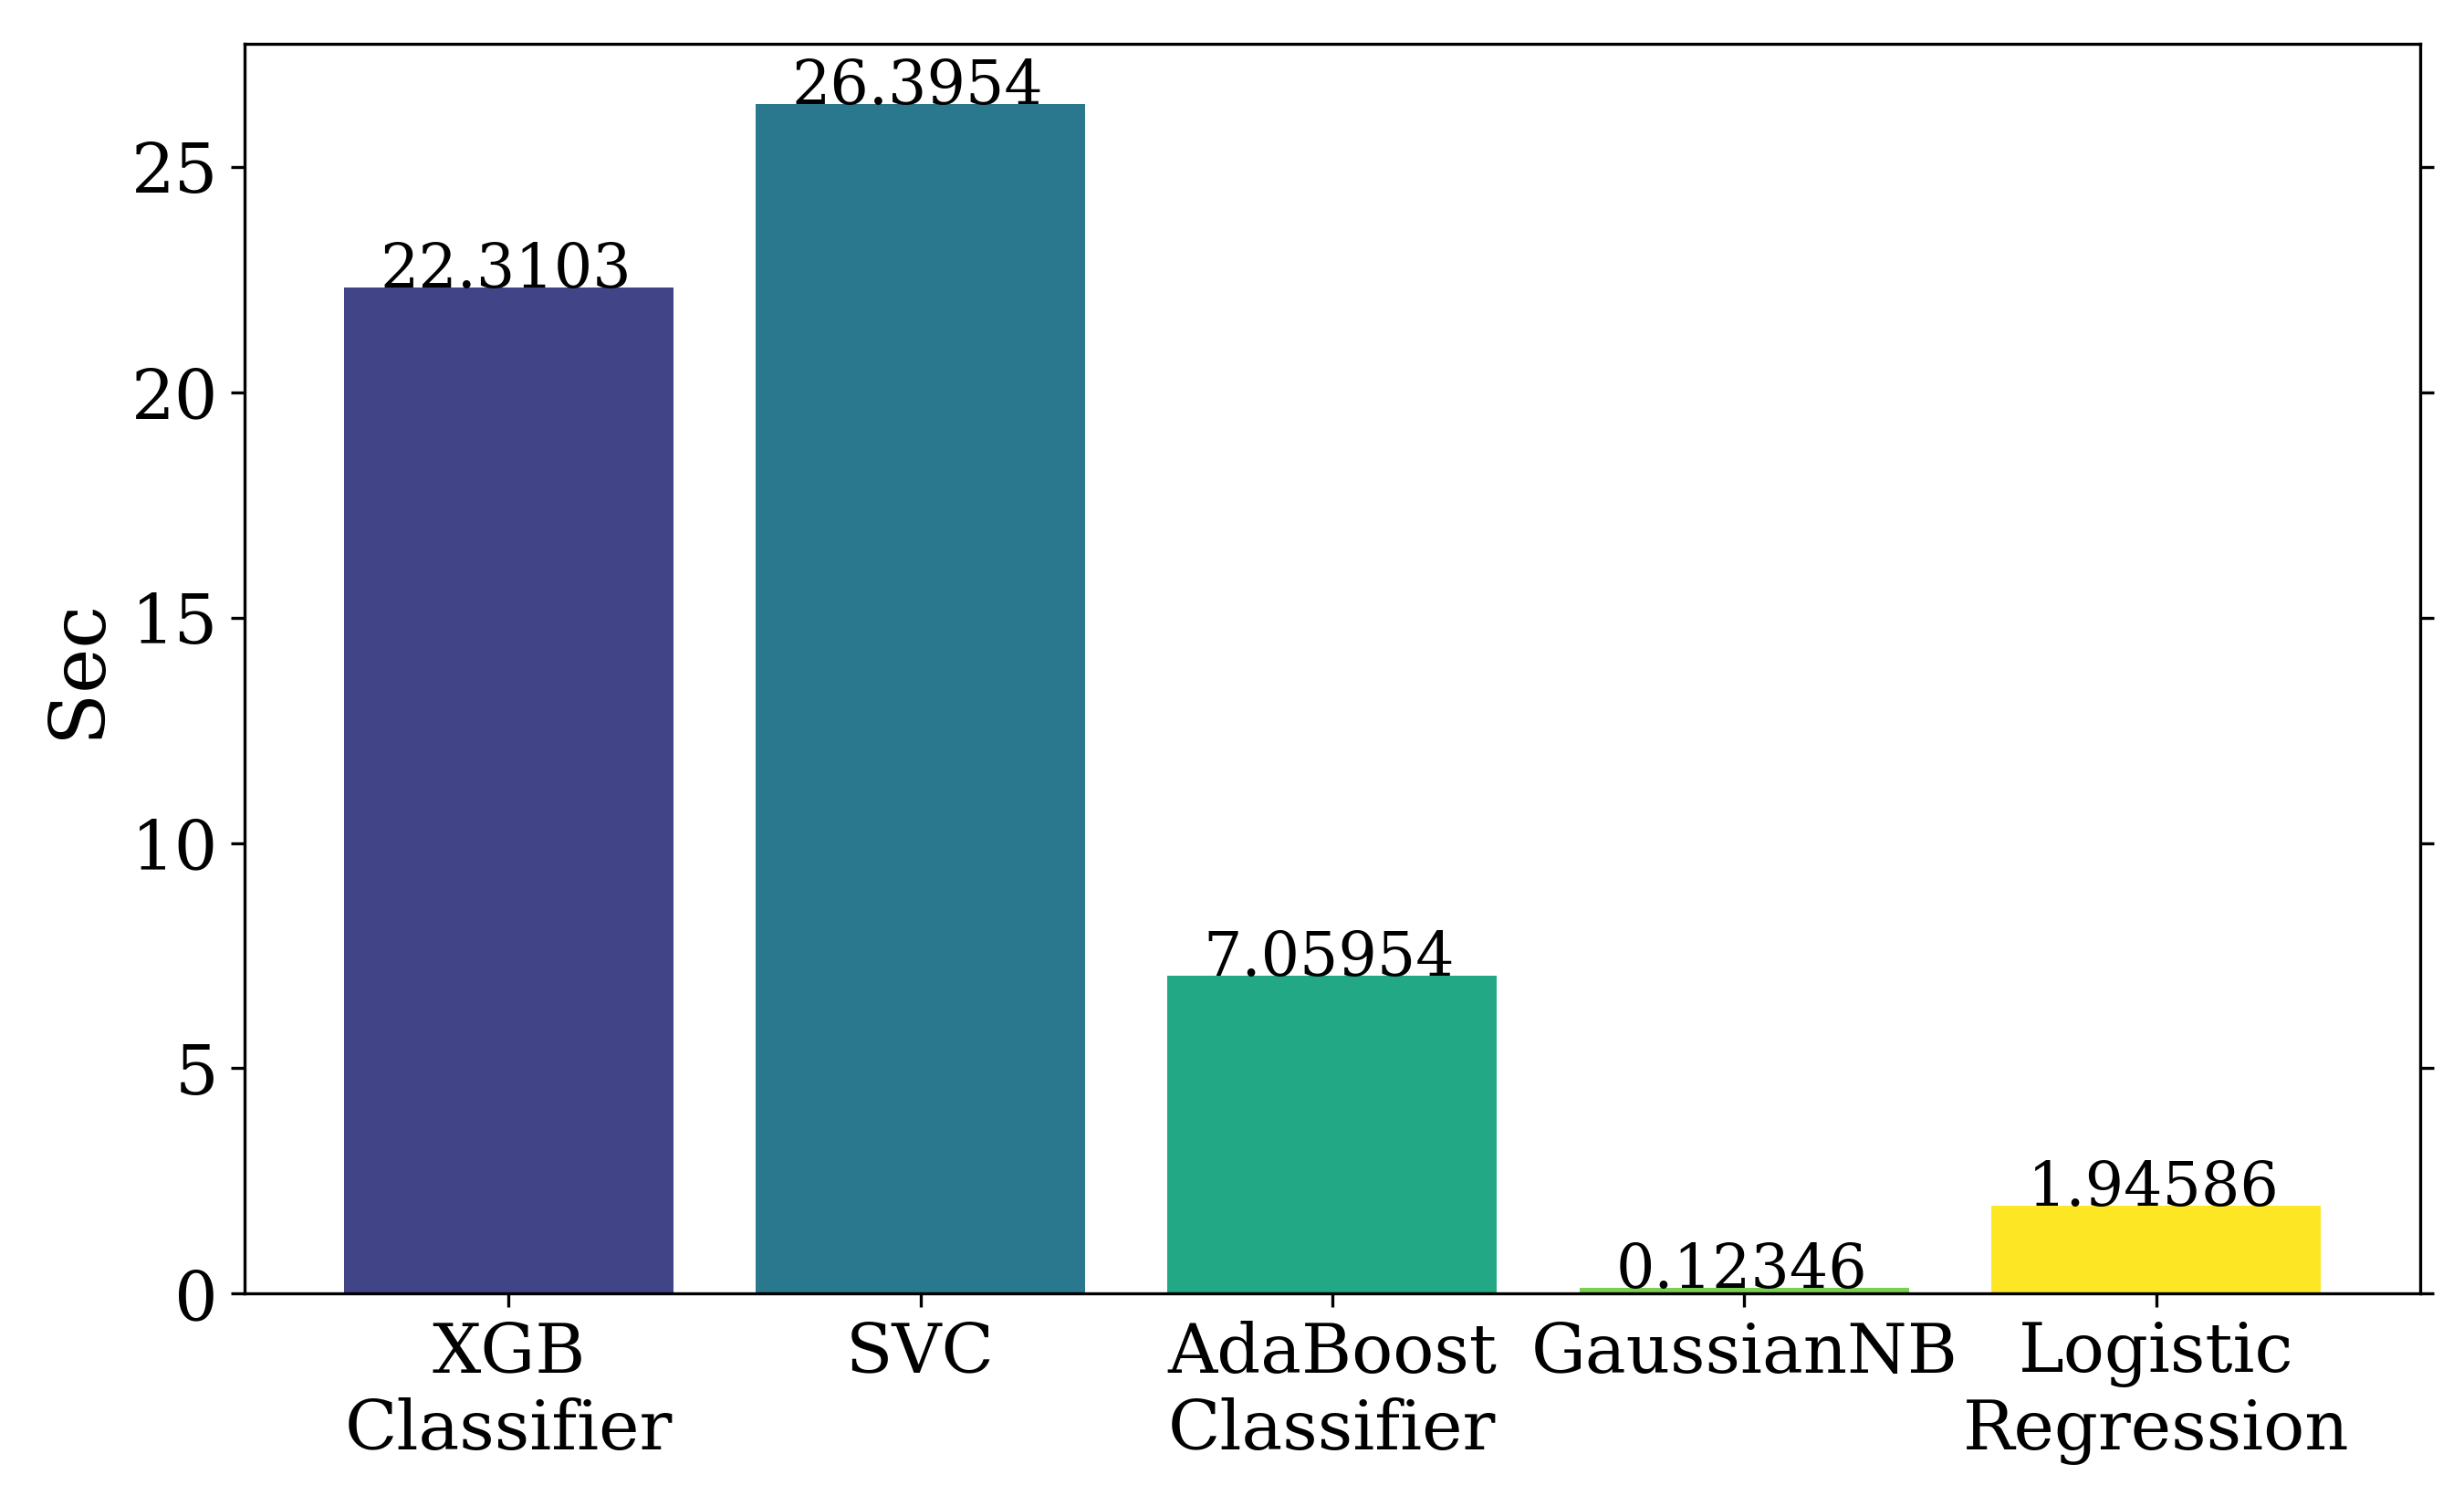
\includegraphics[width=\textwidth]{supporting_images/time_notpca.png}
        \caption{Fitted with the whole data set}
        \label{fig:time_notpca}
    \end{subfigure}
    \hfill
    \begin{subfigure}[t]{0.495\textwidth}
        \centering
        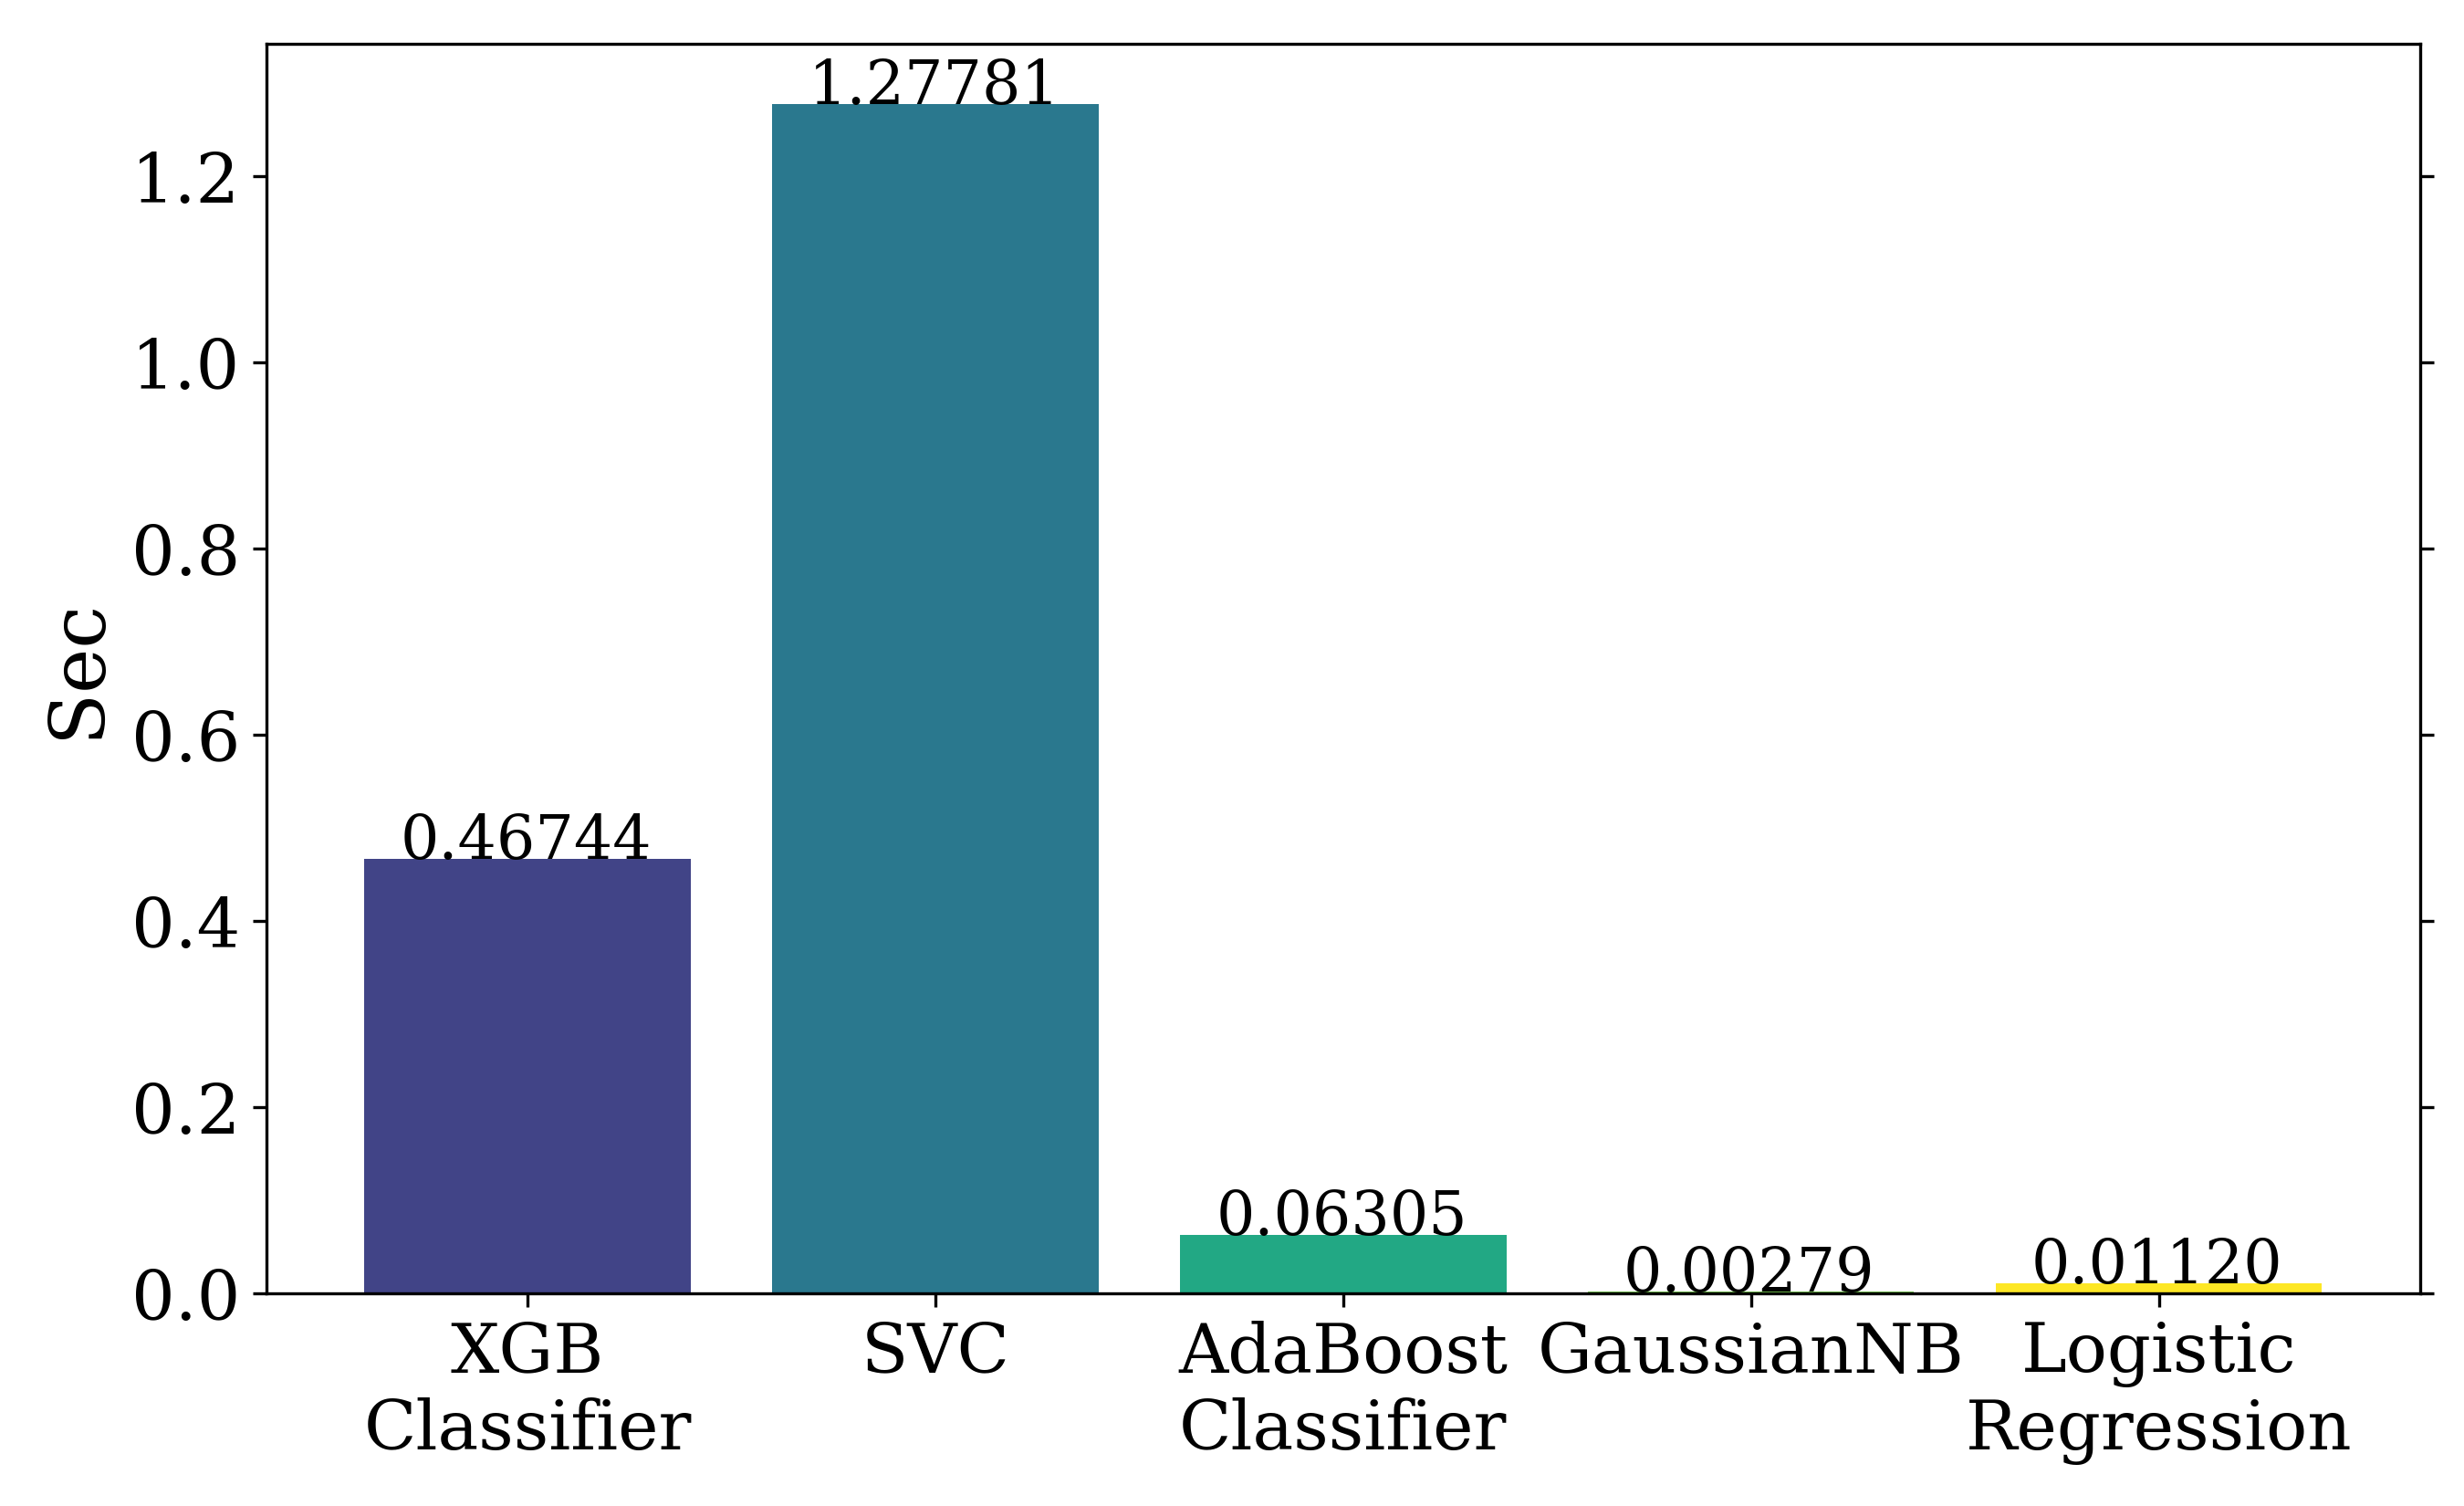
\includegraphics[width=\textwidth]{supporting_images/time_pca.png}
        \caption{Fitted with the transformed PCA data set}
        \label{fig:time_pca}
    \end{subfigure}
    \caption{Training Time}
    \label{fig:time}
\end{figure}

\par
After analyzing the figures, there is one algorithm for each data set that is best qualified be used on them. For the whole data set, the XGB classifier is the most qualified. It had the highest score for testing set accuracy, F1 score, and precision score. It did not score the highest in training set accuracy, but this is because the AdaBoost classifier memorized the training set and scored 100\%. The XGB classifier did take the second longest by a long margin to train, but this cost is acceptable, because the training time is only 13.6637 seconds.

\par
For the transformed PCA data set, the GaussianNB algorithm is the best qualified. The XGB classifier, SVC, GaussianNB and Logistic Regression all scored very similarly in training set accuracy, testing set accuracy, F1 score, and precision score. The Adaboost classifier memorized the training set again and scored 100\%. But GaussianNB had the lowest training time by a several factors, thus it is best qualified for the transformed PCA data set.

\par
For this project, both the XGB classifier with the whole data set and the GaussianNB algorithm with the transformed PCA data set will be used.

%\subsection{Algorithms and Techniques} %Might need to change

\subsection{Benchmark}
\par
The benchmark data set used for this project is the predictions data set (section \ref{Predictions}). This data set is completely independent of the models used in this project, it is calculated by FIRST before every match in real time. The performance of this benchmark will be compared to the true values, the XGB classifier and the GaussianNB algorithm.

\section{Methodology}

\subsection{Data Preprocessing} \label{Actual_Preprocessing}
\par
The transformed PCA data set will be calculated. For this project, the first five dimensions of the PCA transform will be used. Then the same preprocessing will be done to the data sets is the same as done in section \ref{algorithm_selection}, each dimension of the data is scaled to a range [-1, 1]. No other preprocessing is done. No analysis of outliers was done here. This will be made clear why in the results section (\ref{Justification}), but there is no clear line of outliers within the data set.

\subsection{Implementation}
\par
The implementation of both the XGB classifier and the GaussianNB algorithm are identical, with the exception of the algorithms themselves and the PCA transform for the GaussianNB algorithm.

\subsubsection{Week and Ranking Score Selection} \label{week_select}
\par
The first part of implementation is choosing the week or weeks of data the models will be trained on. For this project, the models will be trained on the first week worth of data, first and second weeks worth of data, the first, second, and third weeks worth of data, the first, second, third, and fourth weeks worth of data, and the first, second, third, fourth, and fifth weeks worth of data. The statistics related to ranking score will also be used for one set of tests, but will be removed for the second. This will give a representation of how much data the models need to produce accurate results.

\subsection{Preprocessing}
\par
The same preprocessing in section \ref{Actual_Preprocessing} will occur.

\subsection{Model Training}
\par
For the model training, the data chosen for training will not be divided into training and testing sets. The data chosen for training is the training set and the following week's worth of data will be the testing set. This simulates a real world application of these models. During a week of competition, statistics like OPR, DPR, CCWM, and CPR take between four and five matches to become accurate, thus for the first half of a competition, the current week's worth of data cannot be used.

\subsection{Testing Data Loading and Preprocessing}
\par
After the models have been trained, the testing data will be loaded. This will be the week after the last training data was loaded. So if week one was used for training, then week two will be used for testing. Then the testing data will be preprocessed with the same PCA transform and min-max scaler used for the training data, to avoid any discrepancies between the two data sets.

\subsection{Prediction Calculation and Metric Evaluation}
\par
Now the testing sets are generated, the models will be used to predict the values of the testing sets. Then the metrics (section \ref{Performance_Metrics}) will be evaluated, with the predicted values being tested against the true values.

\subsection{XGB Classifier Feature Weights}
\par
For the XGB classifier, there is a class property called "feature\_importances\_". This outputs the weights of the features used for tree boosters. This will allow for analysis of what features are critical to determining if an alliance will win a match or not.

\subsection{The Coding Process}
\par
Coding all of this functionality took a lot of time. None of it was too complex, just time consuming. The data intake and statistical calculation took about half of my time coding. The models were not hard to use after reading through their documentation. Structuring the code into three different Jupyter notebooks helped with organization. I found a module that allows for a Jupyter notebook to be imported into another notebook just like a module.

\subsection{Model Refinement}
\par
Only the XGB Classifier has hyperparameters that can be tuned. Hours were spend trying to tune the "max\_depth", "learning\_rate", and "n\_estimators" hyperparameters, but no amount of tuning showed significant increase or any increase at all, over the default values. This took me by surprise and I investigated it thoroughly. But the hyperparameters could not be tuned any further. Below is an example of the tuning attempt, with week 1 through 3 as training and week 4 as testing.

\begin{table}[H]
\caption{XGB Classifier Hyperparameter Tuning Attempt}
\centering
\begin{tabular} { |c|c|c| }
\hline
Metric & Default & Best Tuning \\
\hline
Accuracy & 0.90116 & 0.89761 \\
\hline
F1 Score & 0.91256 & 0.90745 \\
\hline
Precision & 0.87400 & 0.86826 \\
\hline
\end{tabular}
\label{table:tuning}
\end{table}

\section{Results} \label{Results}

\subsection{Model Evaluation and Validation}

\subsubsection{Tabular Results from Models and Benchmark} \label{tabular_results}
\par
Below are the tabular results of running the models and comparing them to the benchmark. This was done for the weeks of data outlined in section \ref{week_select}.

\begin{table}[H]
    \caption{Results for Week 1 Training (1396 Samples) and Week 2 Testing (1973 Samples)}
    \centering
    \begin{tabular} { |c|c|c|c|c|c|c|c| }
    \hline
    \multicolumn{2}{|c|}{} & \multicolumn{2}{|c|}{With Ranking Score} & \multicolumn{2}{|c|}{Without Ranking Score} \\
    \hline
    Metric & FIRST & GaussianNB & XGB & GaussianNB & XGB \\
    \hline
    Accuracy & 0.67562 & 0.83223 & 0.90116 & 0.83223 & 0.82057 \\
    \hline
    F1 Score & 0.66437 & 0.84671 & 0.91256 & 0.84671 & 0.83832 \\
    \hline
    Precision & 0.60294 & 0.79269 & 0.87400 & 0.79269 & 0.78183 \\
    \hline
    \end{tabular}
    \label{table:results_week_1}
\end{table}

\begin{table}[H]
    \caption{Results for Week 1 and 2 Training (3369 Samples) and Week 3 Testing (1416 Samples)}
    \centering
    \begin{tabular} { |c|c|c|c|c|c| }
    \hline
    \multicolumn{2}{|c|}{} & \multicolumn{2}{|c|}{With Ranking Score} & \multicolumn{2}{|c|}{Without Ranking Score} \\
    \hline
    Metric & FIRST & GaussianNB & XGB & GaussianNB & XGB \\
    \hline
    Accuracy & 0.69844 & 0.83615 & 0.89477 & 0.83474 & 0.83474 \\
    \hline
    F1 Score & 0.69921 & 0.84959 & 0.90229 & 0.84868 & 0.84717 \\
    \hline
    Precision & 0.63973 & 0.79617 & 0.86269 & 0.79491 & 0.79380 \\
    \hline
    \end{tabular}
    \label{table:results_week_2}
\end{table}

\begin{table}[H]
    \caption{Results for Week 1 Through 3 Training (4785 Samples) and Week 4 Testing (1586 Samples)}
    \centering
    \begin{tabular} { |c|c|c|c|c|c|c|c| }
    \hline
    \multicolumn{2}{|c|}{} & \multicolumn{2}{|c|}{With Ranking Score} & \multicolumn{2}{|c|}{Without Ranking Score} \\
    \hline
    Metric & FIRST & GaussianNB & XGB & GaussianNB & XGB \\
    \hline
    Accuracy & 0.72572 & 0.83228 & 0.91424 & 0.83165 & 0.82534 \\
    \hline
    F1 Score & 0.72227 & 0.83271 & 0.91668 & 0.83189 & 0.82855 \\
    \hline
    Precision & 0.65907 & 0.77929 & 0.88194 & 0.77844 & 0.77324 \\
    \hline
    \end{tabular}
    \label{table:results_week_3}
\end{table}

\begin{table}[H]
    \caption{Results for Week 1 Through 4 Training (6371 Samples) and Week 5 Testing (1856 Samples)}
    \centering
    \begin{tabular} { |c|c|c|c|c|c|c|c| }
    \hline
    \multicolumn{2}{|c|}{} & \multicolumn{2}{|c|}{With Ranking Score} & \multicolumn{2}{|c|}{Without Ranking Score} \\
    \hline
    Metric & FIRST & GaussianNB & XGB & GaussianNB & XGB \\
    \hline
    Accuracy & 0.72737 & 0.83620 & 0.91702 & 0.83566 & 0.84105 \\
    \hline
    F1 Score & 0.73260 & 0.83624 & 0.91969 & 0.83590 & 0.84321 \\
    \hline
    Precision & 0.67185 & 0.78532 & 0.88680 & 0.78484 & 0.79244 \\
    \hline
    \end{tabular}
    \label{table:results_week_4}
\end{table}

\begin{table}[H]
    \caption{Results for Week 1 Through 5 Training (8227 Samples) and Week 6 Testing (968 Samples)}
    \centering
    \begin{tabular} { |c|c|c|c|c|c|c|c| }
    \hline
    \multicolumn{2}{|c|}{} & \multicolumn{2}{|c|}{With Ranking Score} & \multicolumn{2}{|c|}{Without Ranking Score} \\
    \hline
    Metric & FIRST & GaussianNB & XGB & GaussianNB & XGB \\
    \hline
    Accuracy & 0.71900 & 0.81611 & 0.91735 & 0.81611 & 0.82644 \\
    \hline
    F1 Score & 0.70961 & 0.81873 & 0.91475 & 0.81873 & 0.82892 \\
    \hline
    Precision & 0.64652 & 0.76227 & 0.88215 & 0.76227 & 0.77388 \\
    \hline
    \end{tabular}
    \label{table:results_week_5}
\end{table}

\subsubsection{PCA Result Plots} \label{pca_results}
\par
Below are plots using the first two dimensions of a PCA transformation for week one through week five of training data and week six of testing.

%True Values
\begin{figure}[H]
    \centering
    \begin{subfigure}[t]{0.495\textwidth}
        \centering
        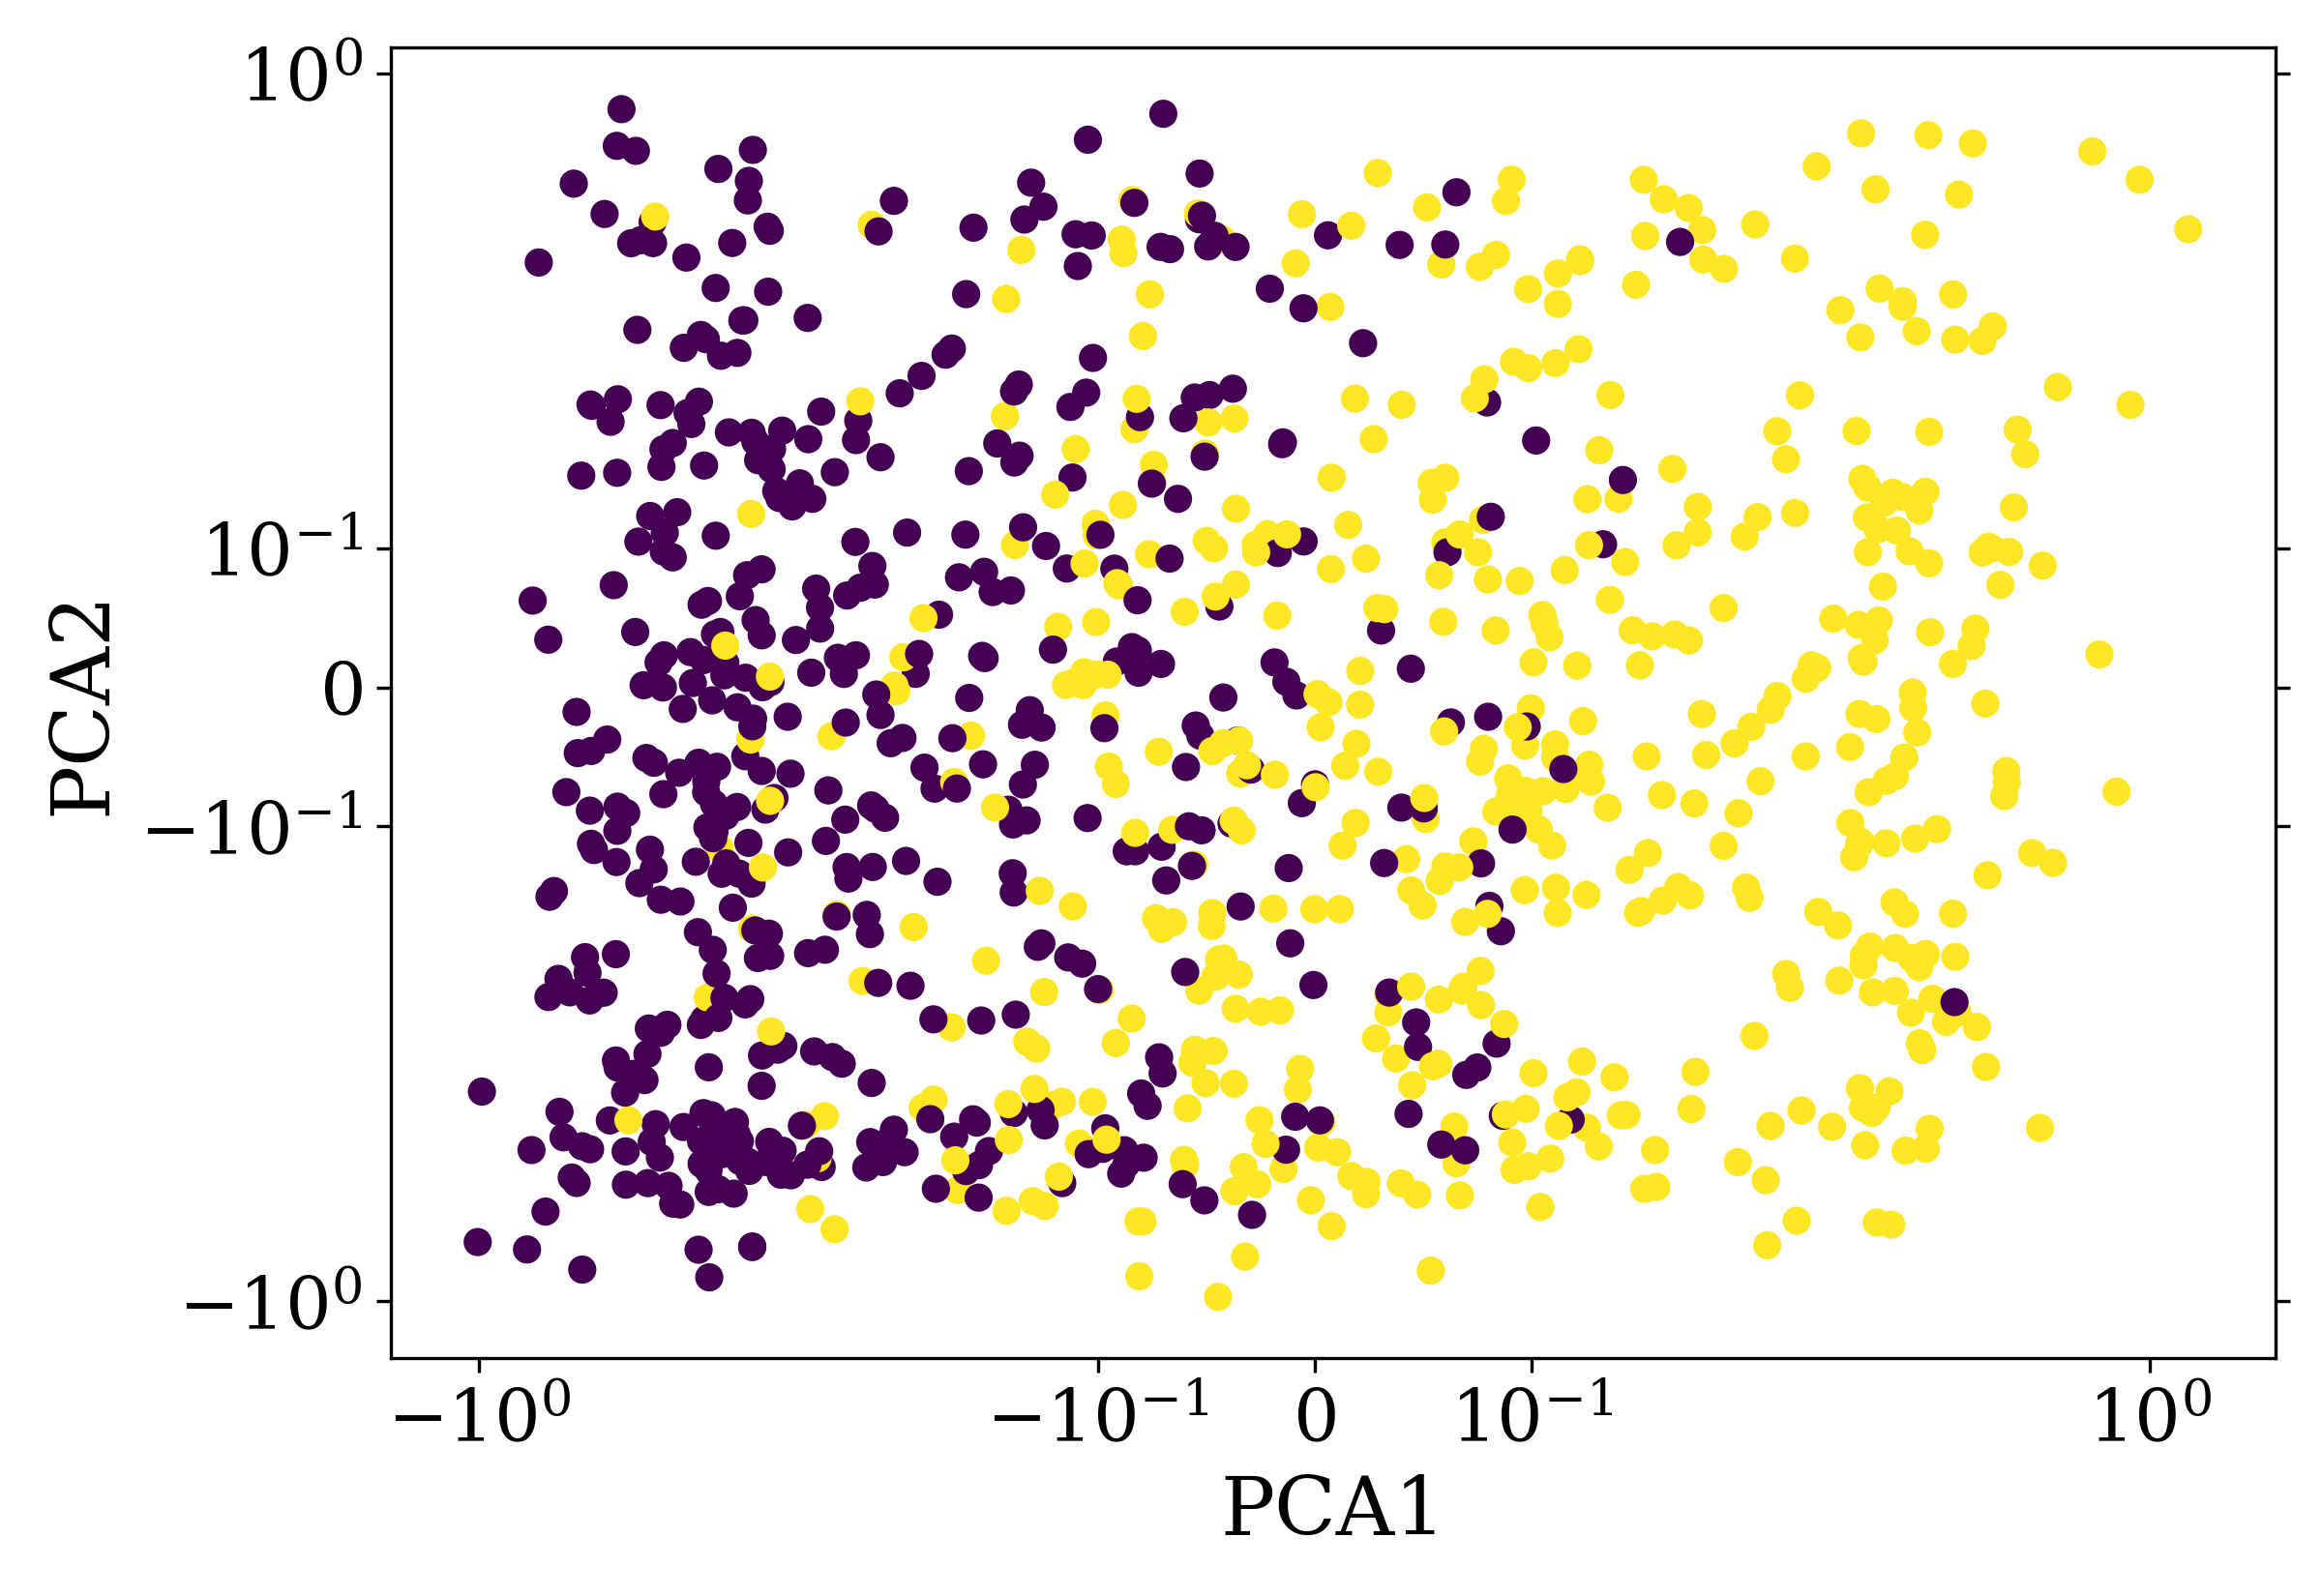
\includegraphics[width=\textwidth]{results/GaussianNB_True_Values_Week_6_With_RS_True.png}
        \caption{True Values (Loss-Purple, Win-Yellow)}
        \label{fig:true_values_sub}
    \end{subfigure}
    \caption{True Values}
    \label{fig:true_values}
\end{figure}

%FIRST Values / Diff First True
\begin{figure}[H]
    \centering
    \begin{subfigure}[t]{0.495\textwidth}
        \centering
        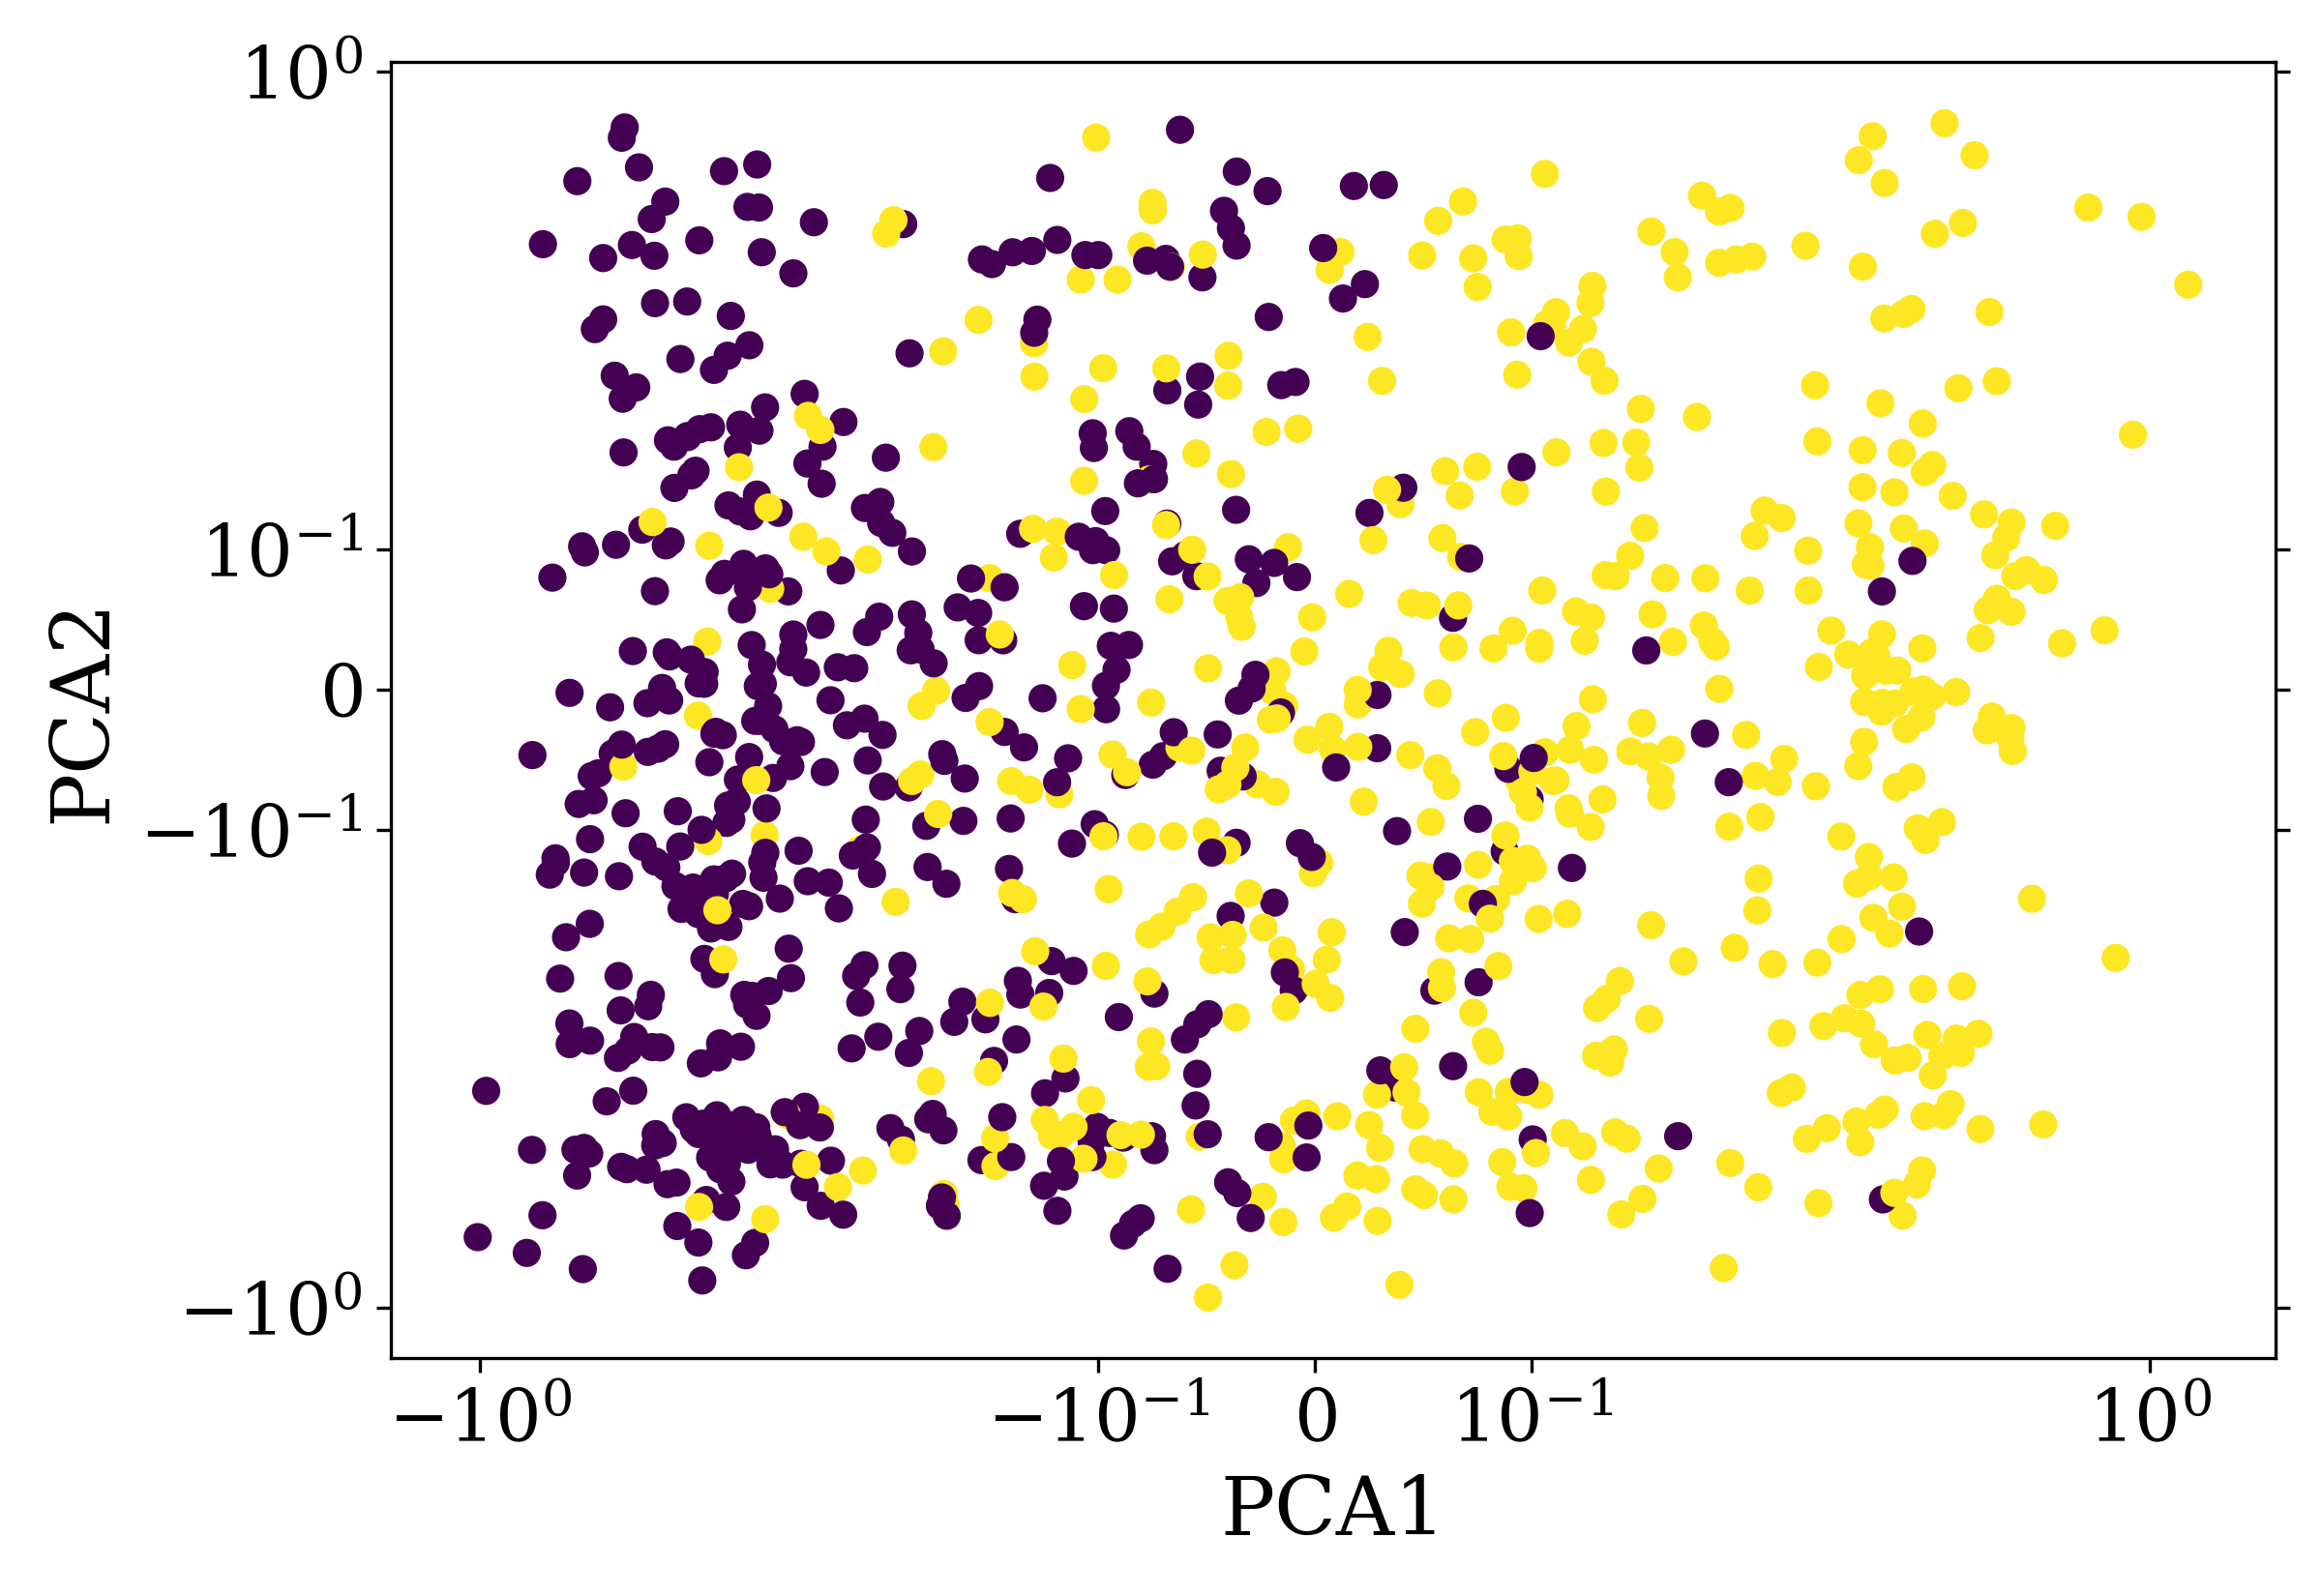
\includegraphics[width=\textwidth]{results/GaussianNB_FIRST_Week_6_With_RS_True.png}
        \caption{FIRST Values (Loss-Purple, Win-Yellow)}
        \label{fig:first_values}
    \end{subfigure}
    \hfill
    \begin{subfigure}[t]{0.495\textwidth}
        \centering
        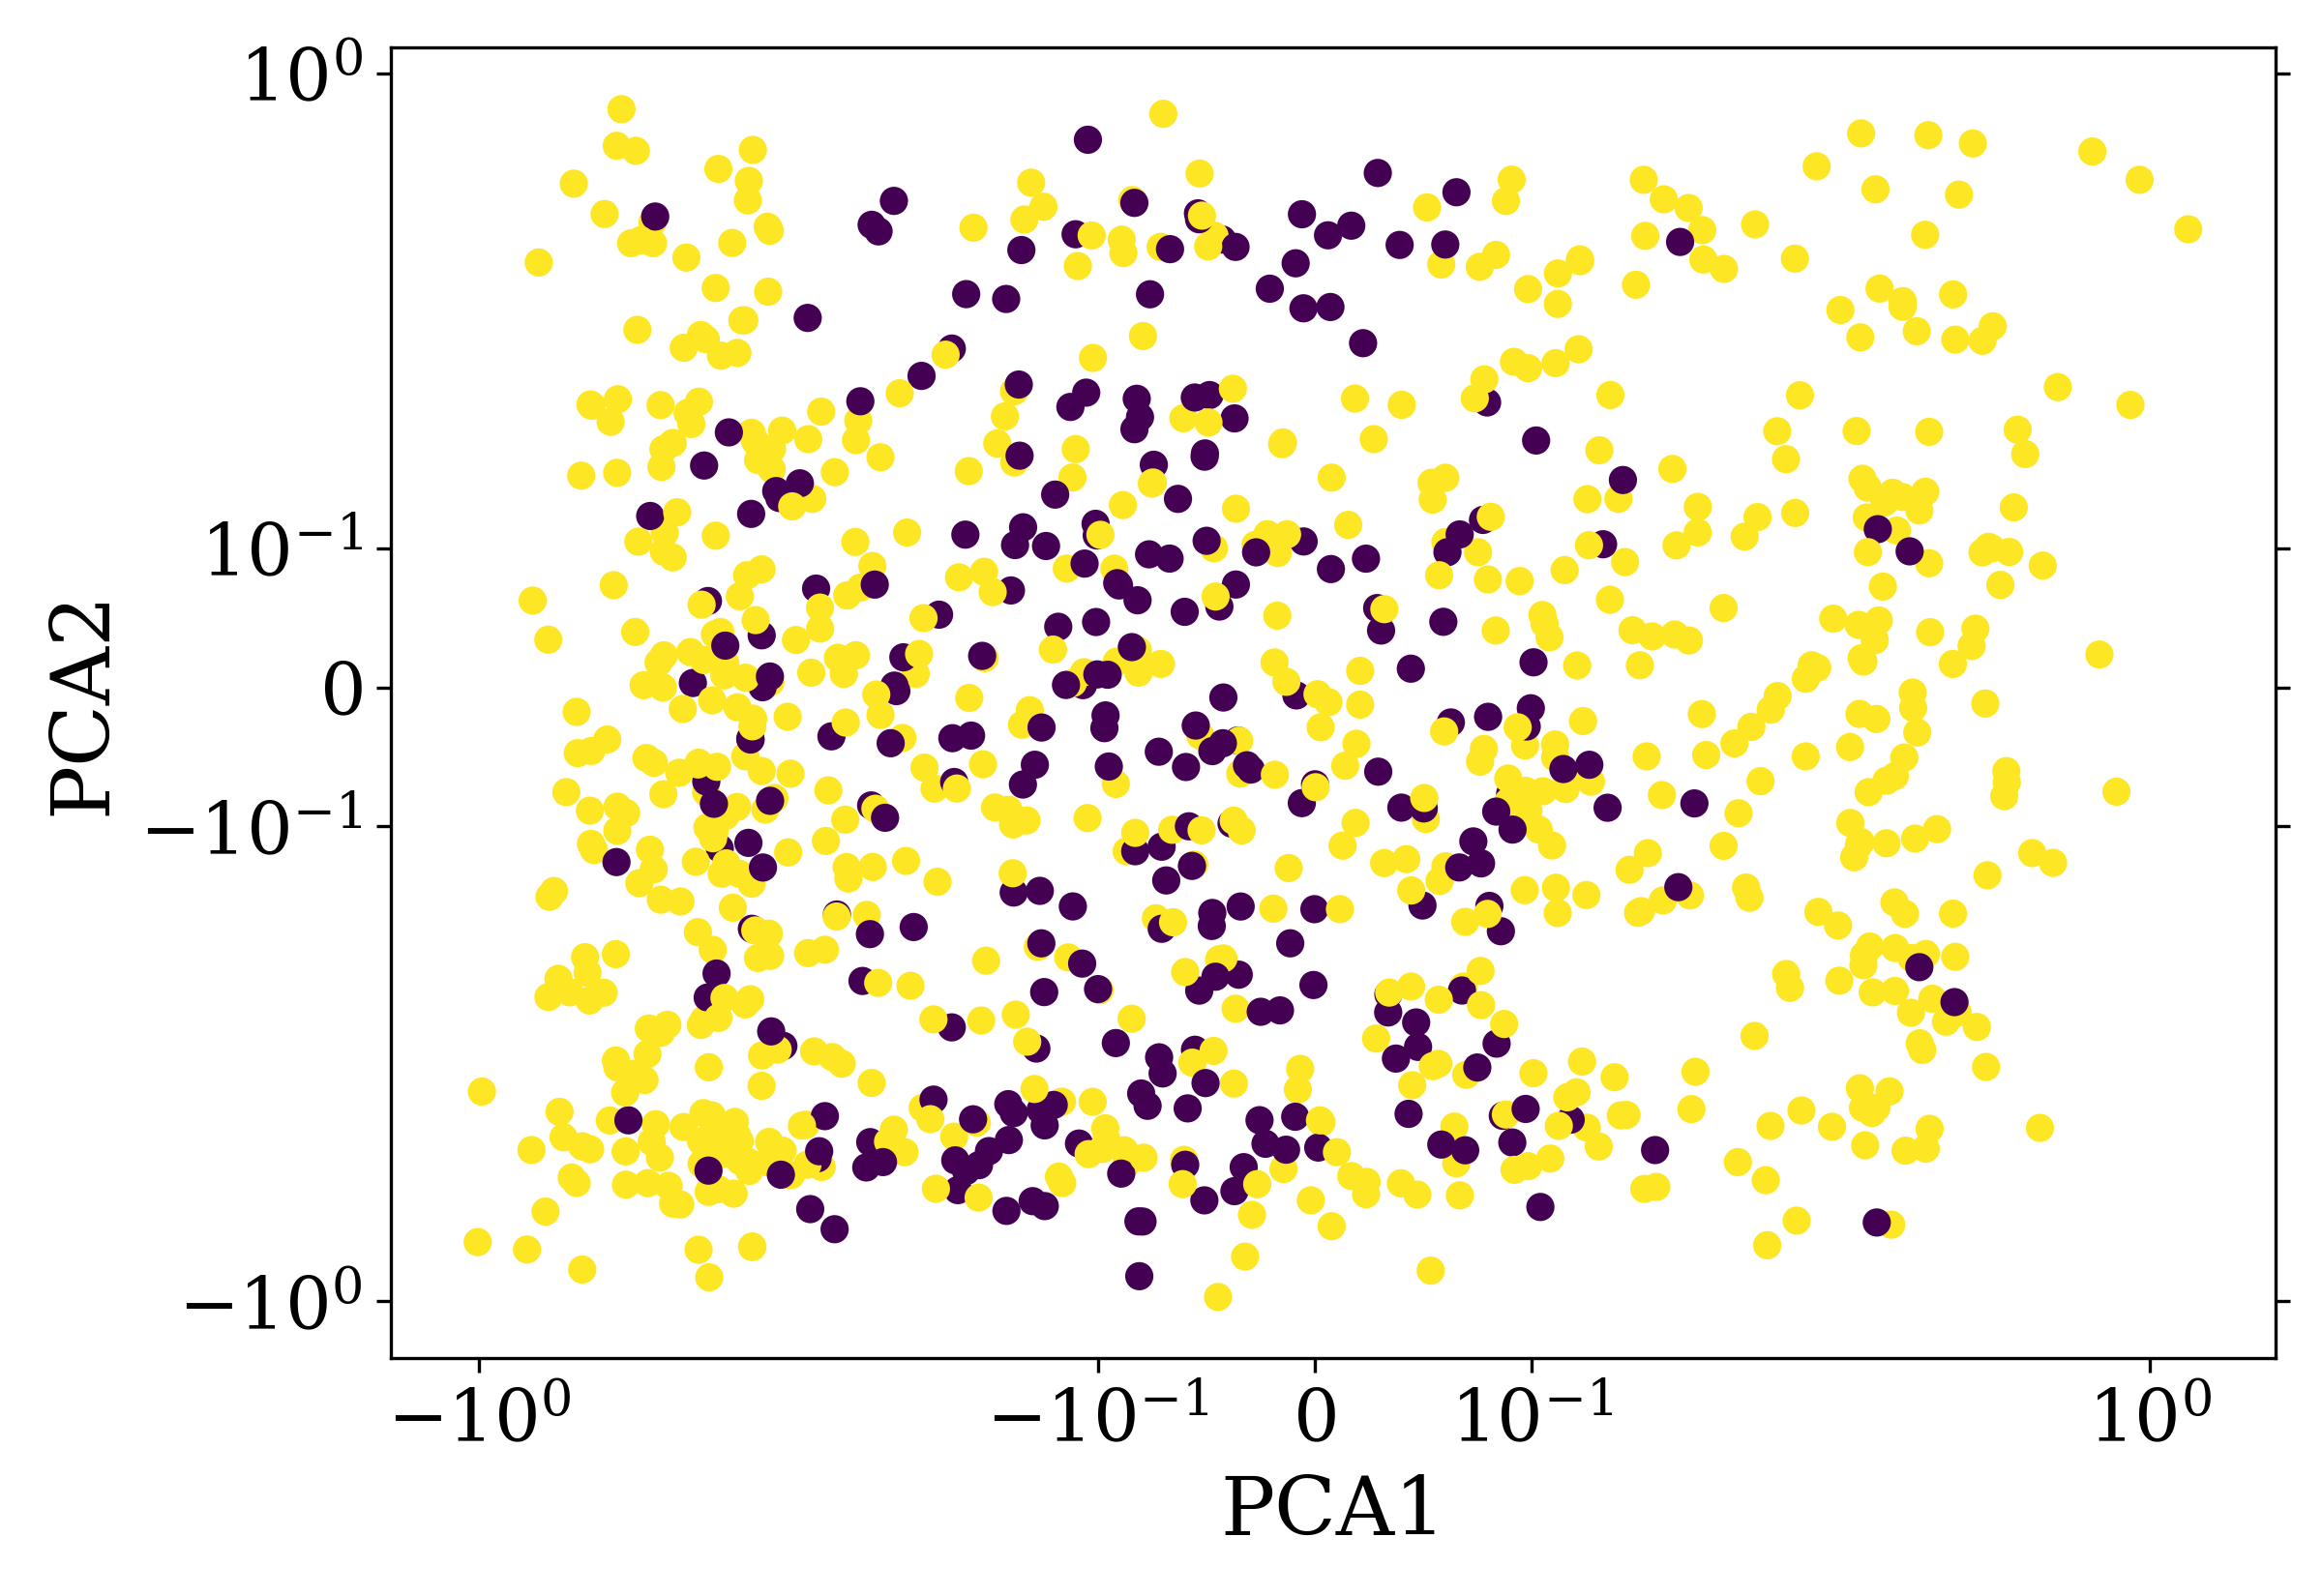
\includegraphics[width=\textwidth]{results/GaussianNB_Diff_FIRST_True_Week_6_With_RS_True.png}
        \caption{Difference Between True Values and FIRST Values (Difference-Purple)}
        \label{fig:diff_first_true}
    \end{subfigure}
    \caption{FIRST Values}
    \label{fig:first_values_fig}
\end{figure}

%GaussianNB Values
\begin{figure}[H]
    \centering
    \begin{subfigure}[t]{0.495\textwidth}
        \centering
        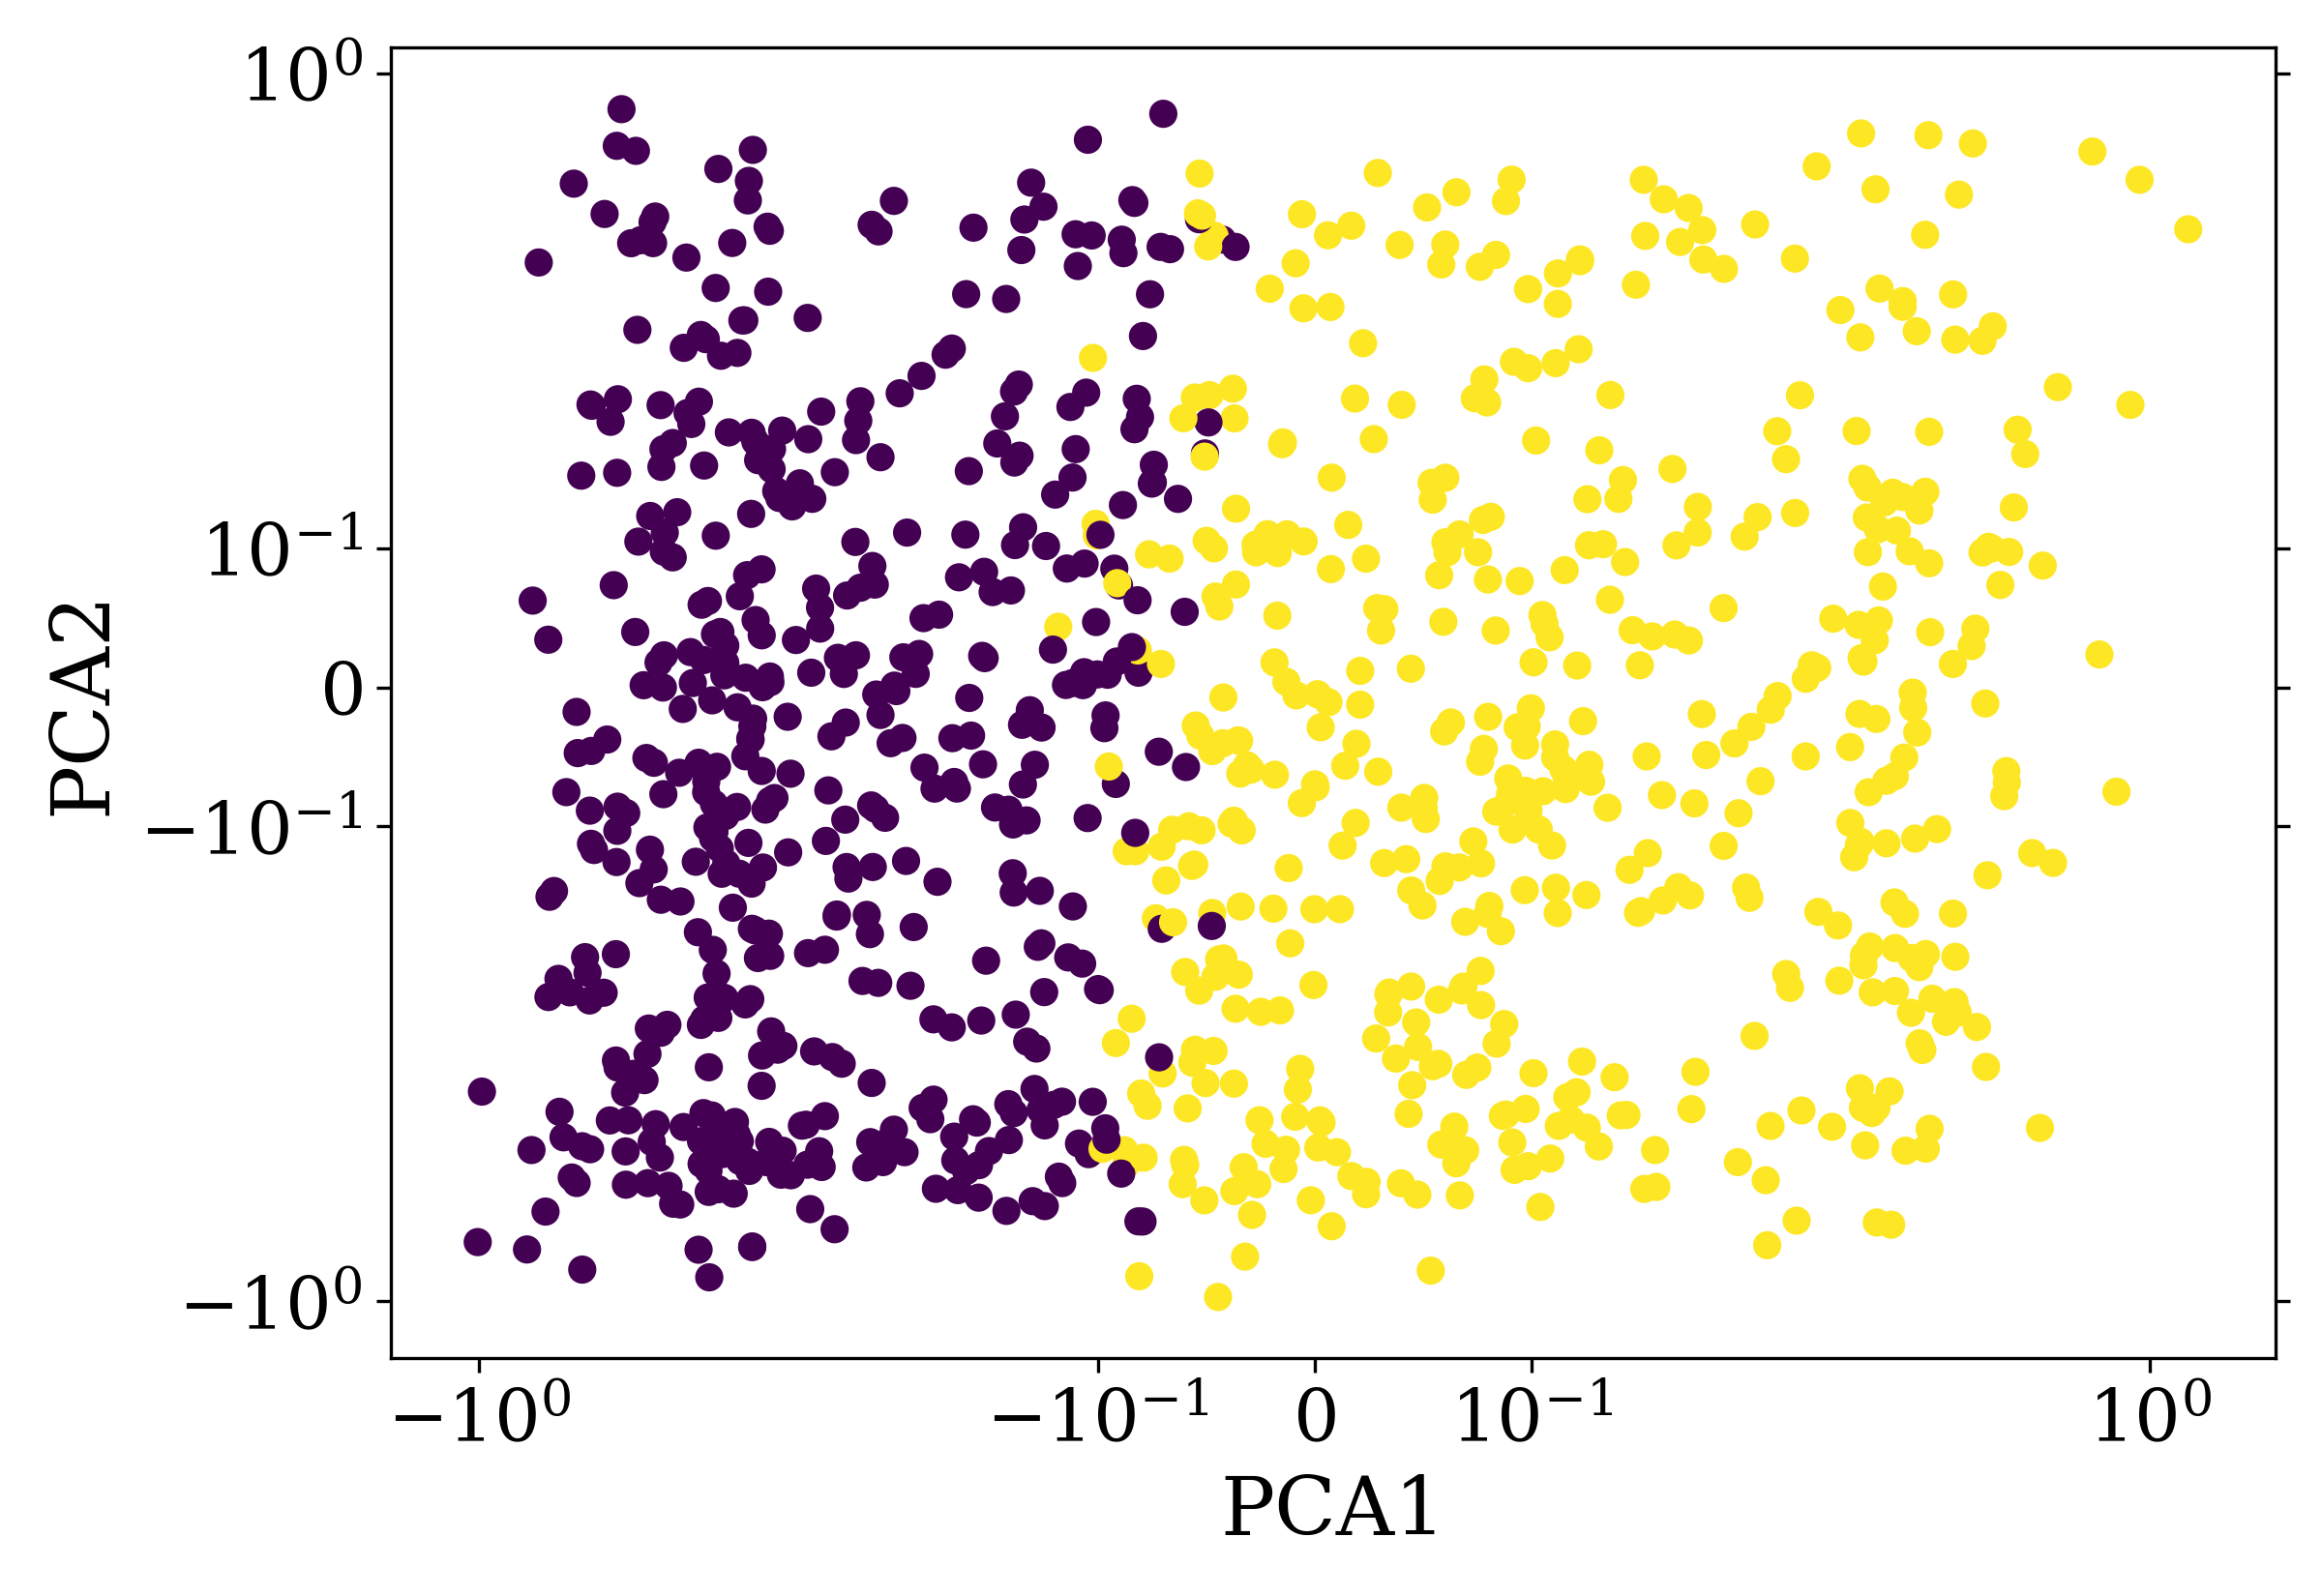
\includegraphics[width=\textwidth]{results/GaussianNB_Gauss_Week_6_With_RS_True.png}
        \caption{GaussianNB Values (Loss-Purple, Win-Yellow)}
        \label{fig:gaussiannb_values}
    \end{subfigure}
    \hfill
    \begin{subfigure}[t]{0.495\textwidth}
        \centering
        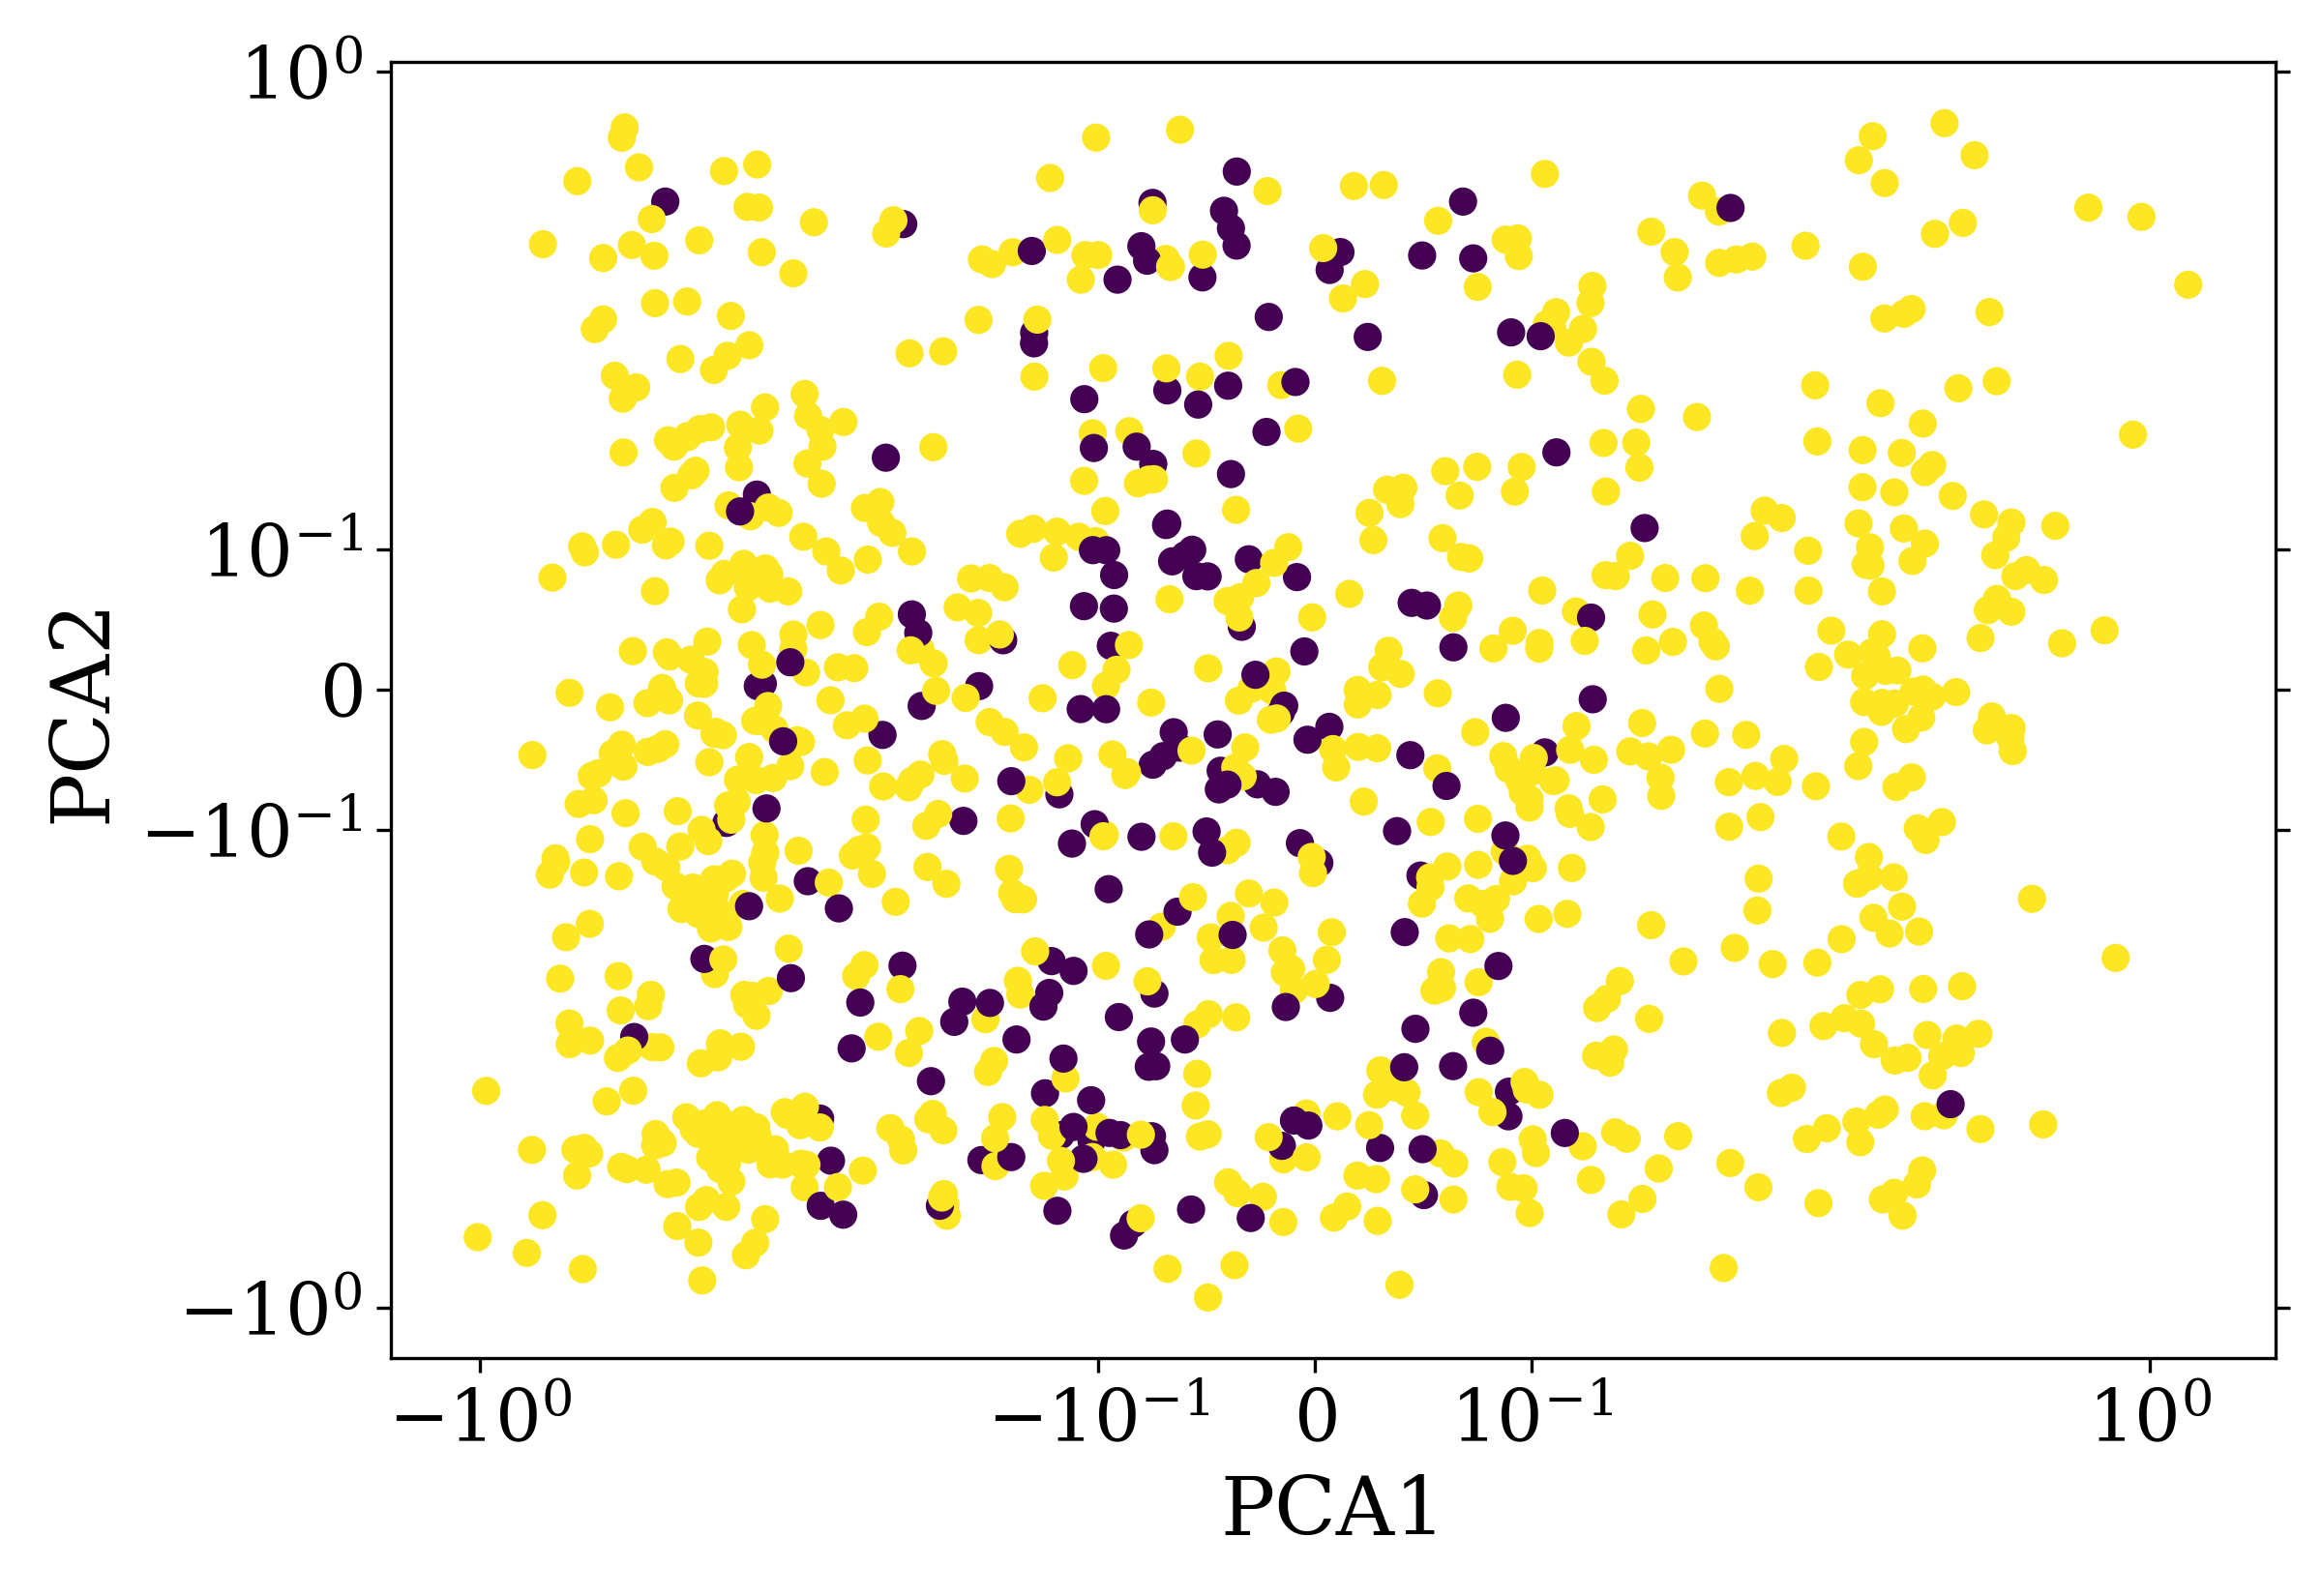
\includegraphics[width=\textwidth]{results/GaussianNB_Diff_Gauss_True_Week_6_With_RS_True.png}
        \caption{Difference Between True Values and GaussianNB Values (Difference-Purple)}
        \label{fig:diff_gaussiannb_true}
    \end{subfigure}
    \caption{GaussianNB Values}
    \label{fig:guassiannb_values_fig}
\end{figure}

%XGB
\begin{figure}[H]
    \centering
    \begin{subfigure}[t]{0.495\textwidth}
        \centering
        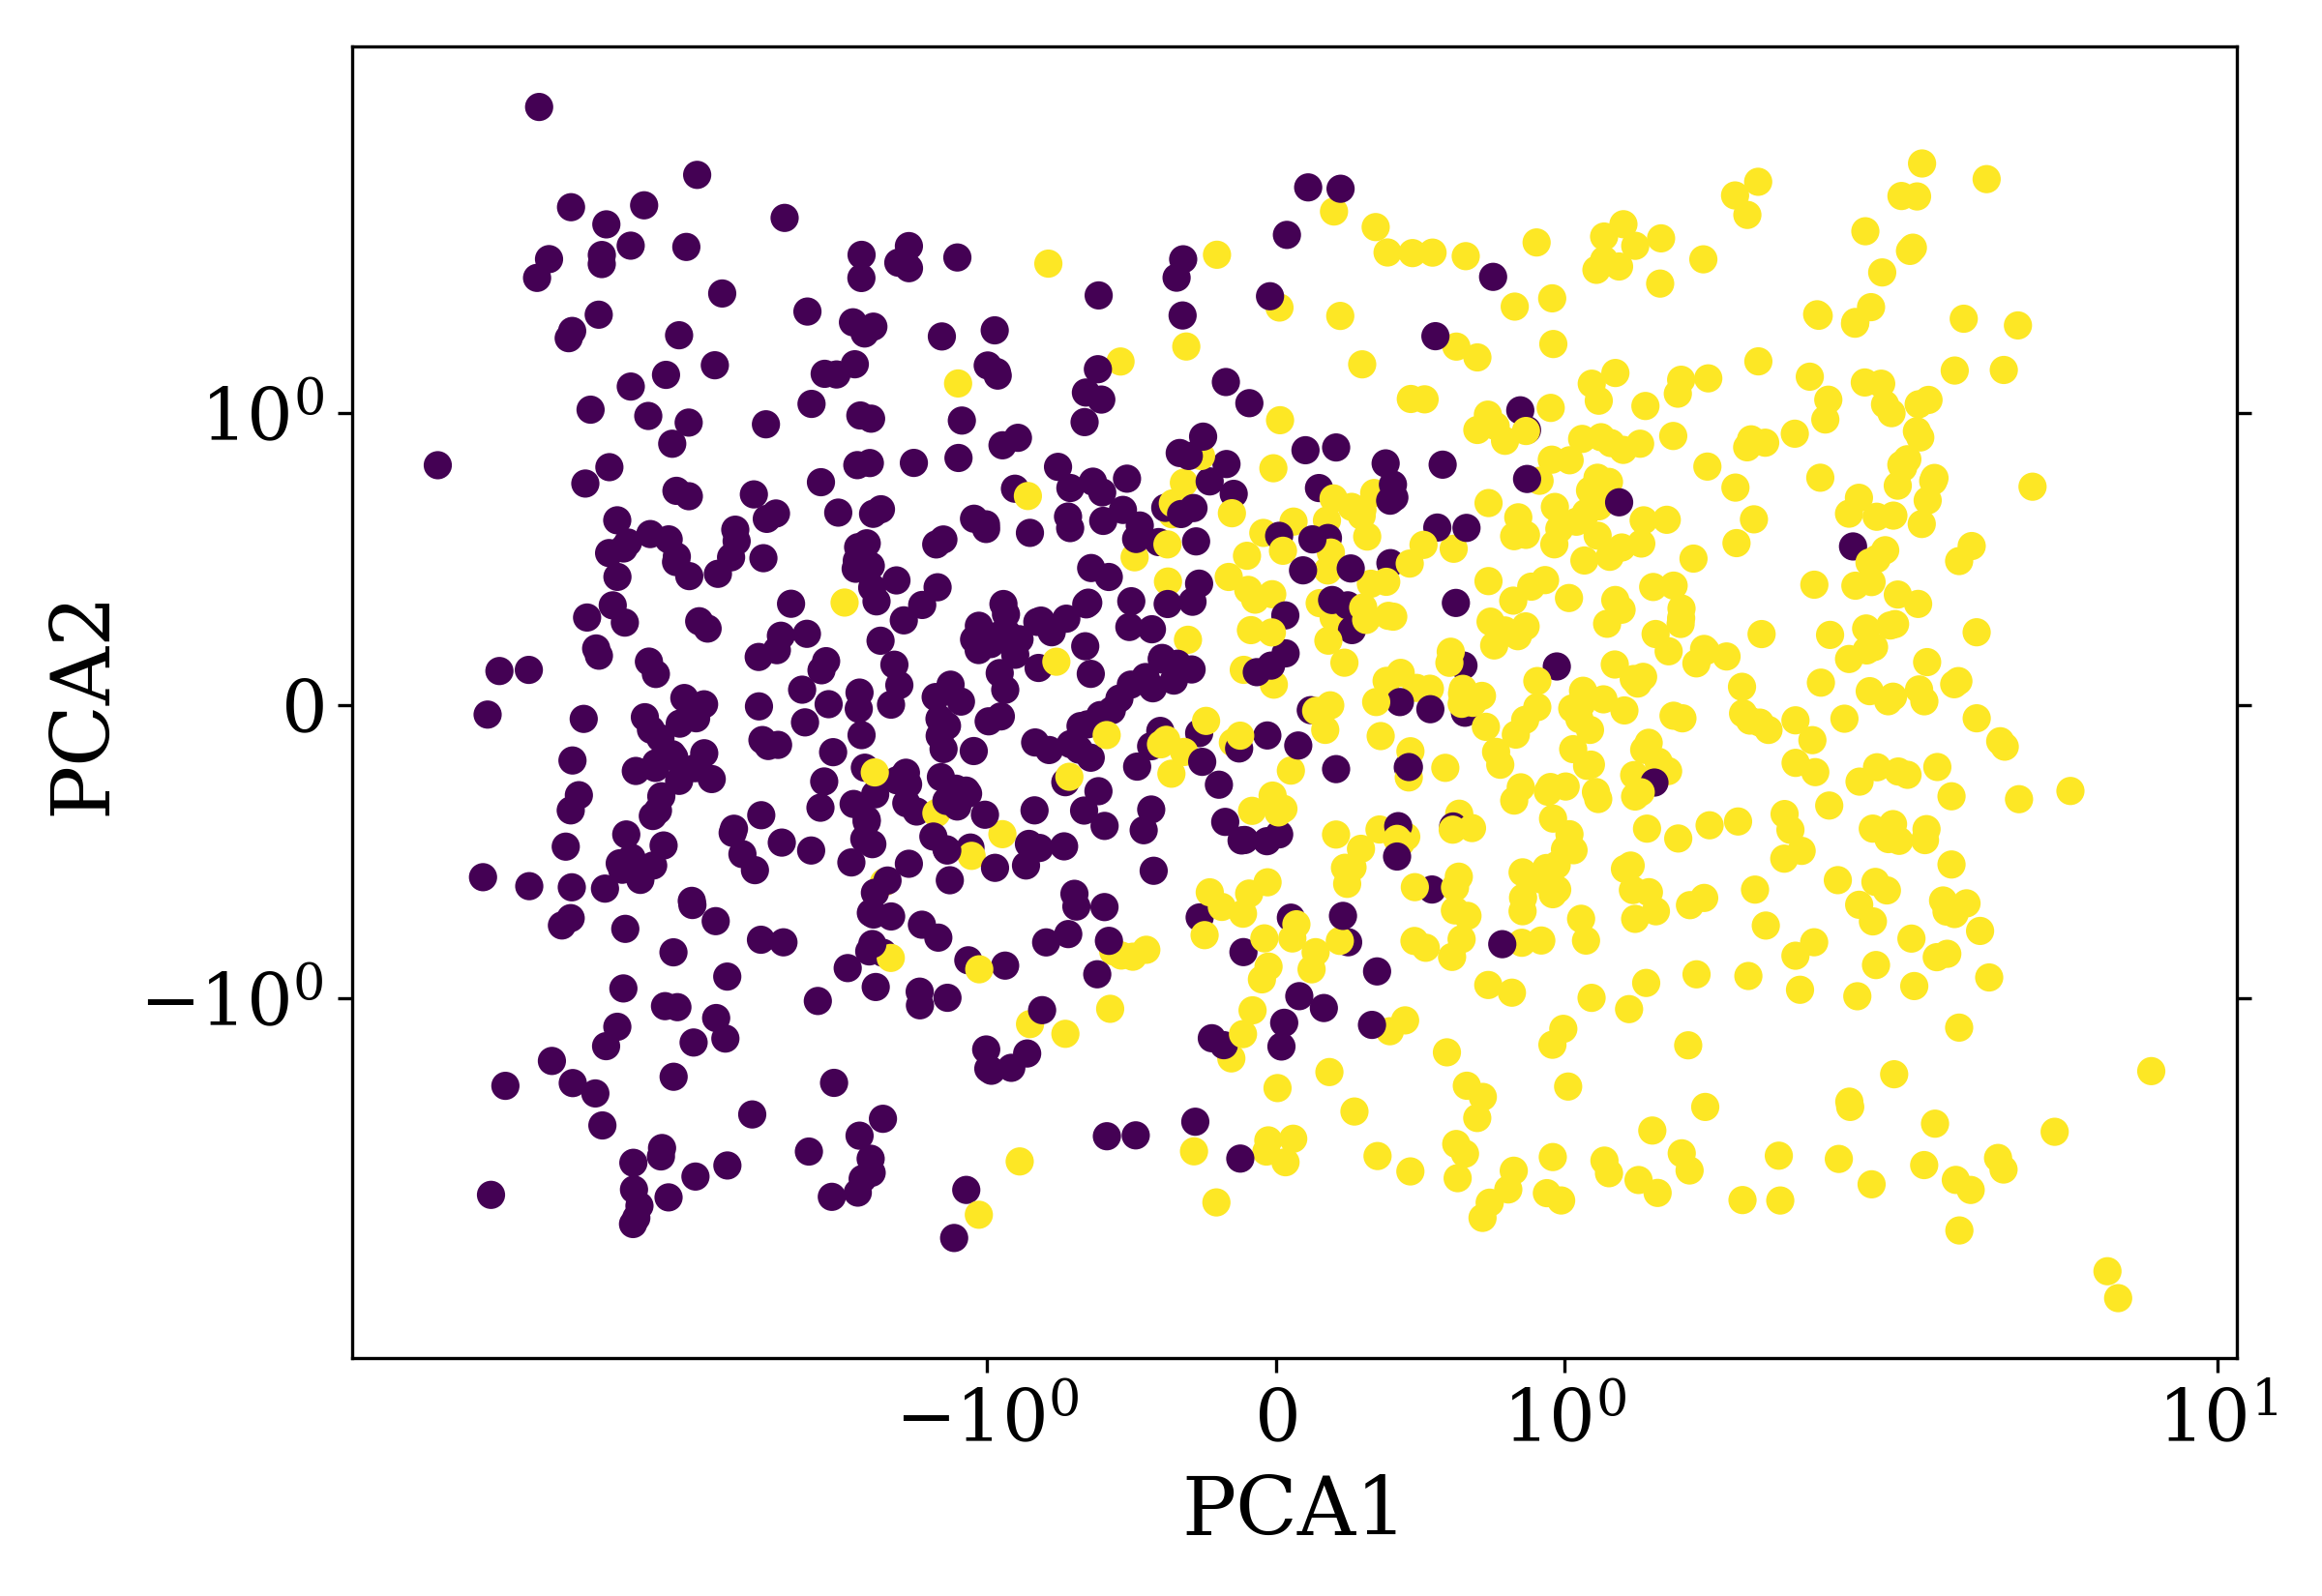
\includegraphics[width=\textwidth]{results/XGB_XGB_Week_6_With_RS_True.png}
        \caption{XGB Values (Loss-Purple, Win-Yellow)}
        \label{fig:xgb_values}
    \end{subfigure}
    \hfill
    \begin{subfigure}[t]{0.495\textwidth}
        \centering
        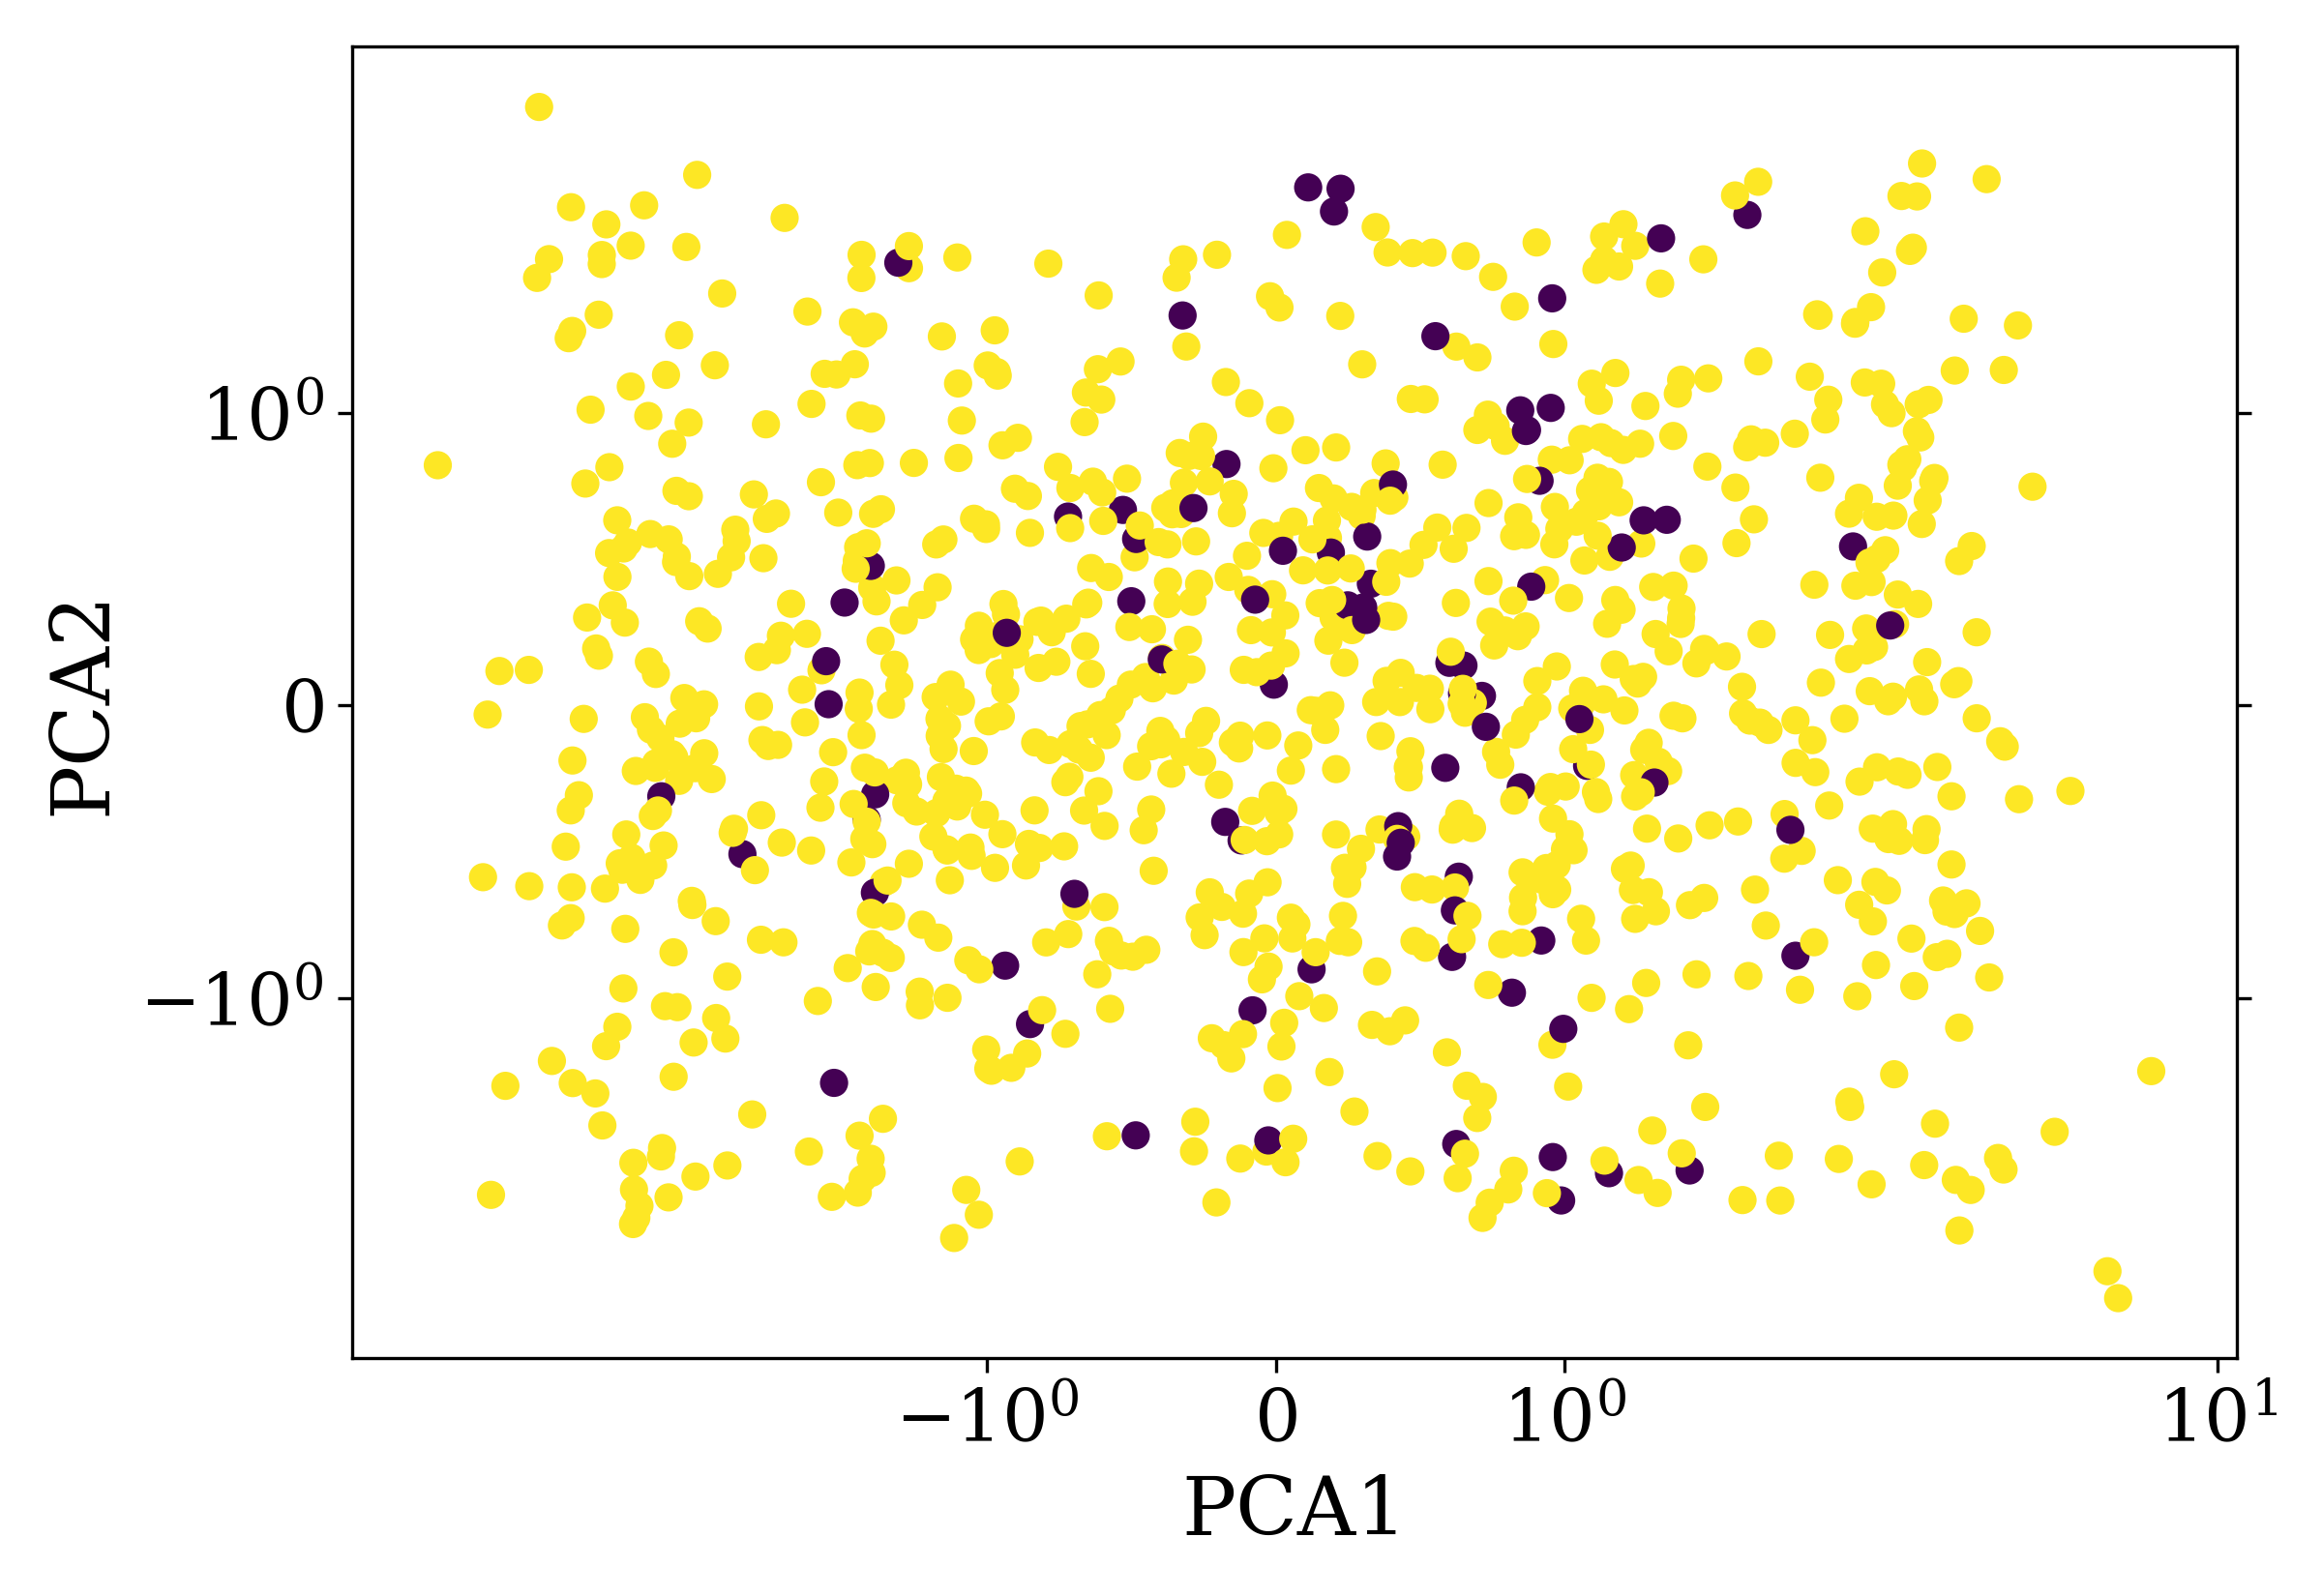
\includegraphics[width=\textwidth]{results/XGB_Diff_XGB_True_Week_6_With_RS_True.png}
        \caption{Difference Between True Values and XGB Values (Difference-Purple)}
        \label{fig:diff_xgb_first}
    \end{subfigure}
    \caption{XGB Values}
    \label{fig:xgb_values_fig}
\end{figure}

\subsubsection{Feature Importance Results} \label{feature_results}
\par
The feature importance for week 2 and week 6 of testing with ranking score and without ranking score are below.

\begin{table}[H]
    \caption{Feature importances for week 2}
    \centering
    \begin{tabular} { |c|c|c|c|c| }
    \hline
    Index & \multicolumn{2}{|c|}{With Ranking Score} & \multicolumn{2}{|c|}{Without Ranking Score} \\
    \hline
    1 & tba\_rpEarned\_CCWM & 0.11202 & CCWM & 0.10754 \\
    \hline
    2 & tba\_rpEarned\_OPR & 0.06260 & OPR & 0.03210 \\
    \hline
    3 & tba\_rpEarned\_DPR & 0.03789 & position5\_B\_Ramparts\_CCWM & 0.01444 \\
    \hline
    4 & teleopDefensesBreached\_CCWM & 0.02965 & Auto\_Crossed\_a & 0.01444 \\
    \hline
    5 & tba\_rpEarned\_CPR & 0.01976 & position4crossings\_CCWM & 0.01284 \\
    \hline
    6 & position3\_D\_RoughTerrain\_CPR & 0.01647 & Scale/Challenge\_a & 0.01284 \\
    \hline
    7 & teleopDefensesBreached\_DPR & 0.01317 & teleopTowerCaptured\_CCWM & 0.01284 \\
    \hline
    8 & teleopDefensesBreached\_CPR & 0.01317 & towerFaceA\_None\_CCWM & 0.01123 \\
    \hline
    9 & autoCrossingPoints\_DPR & 0.01317 & autoPoints\_OPR & 0.01123 \\
    \hline
    10 & autoPoints\_DPR & 0.01153 & teleopPoints\_CCWM & 0.01123 \\
    \hline
    \end{tabular}
    \label{table:feature_importance_week_2}
\end{table}

\begin{table}[H]
    \caption{Feature importances for week 6}
    \centering
    \resizebox{\textwidth}{!}{%
    \begin{tabular} { |c|c|c|c|c| }
    \hline
    Index & \multicolumn{2}{|c|}{With Ranking Score} & \multicolumn{2}{|c|}{Without Ranking Score} \\
    \hline
    1 & tba\_rpEarned\_CCWM & 0.13253 & CCWM & 0.12878 \\
    \hline
    2 & tba\_rpEarned\_OPR & 0.08132 & OPR & 0.10151 \\
    \hline
    3 & teleopDefensesBreached\_CCWM & 0.08132 & position1crossings\_CCWM & 0.01818 \\
    \hline
    4 & teleopTowerCaptured\_CCWM & 0.04518 & teleopTowerCaptured\_CCWM & 0.01818 \\
    \hline
    5 & tba\_rpEarned\_DPR & 0.04066 & towerFaceA\_Scaled\_CCWM & 0.016666 \\
    \hline
    6 & tba\_rpEarned\_CPR & 0.02710 & CPR & 0.01515 \\
    \hline
    7 & OPR & 0.02108 & teleopDefensesBreached\_CCWM & 0.01515 \\
    \hline
    8 & towerFaceA\_Scaled\_CCWM & 0.01807 & towerEndStrength\_DPR & 0.01363 \\
    \hline
    9 & teleopDefensesBreached\_OPR & 0.01506 & techFoulCount\_CCWM & 0.01212 \\
    \hline
    10 & autoPoints\_DPR & 0.01355 & towerFaceC\_Challenged\_CCWM & 0.01060 \\
    \hline
    \end{tabular}
    }
    \label{table:feature_importance_week_6}
\end{table}

\subsection{Justification} \label{Justification}
\par
From the section above, we can conclude the following:
\begin{itemize}
    \item From section \ref{tabular_results}, Tabular Results from Models and Benchmark
    \begin{itemize}
        \item FIRST's predictions got better the first three weeks, then stayed about the same, while the other models stayed the about the same the whole time
        \item All of the models, with and without ranking score, preformed better than the FIRST's predictions, the benchmark.
        \item For GaussianNB and XGB without ranking score, both preformed about equal for all three metrics.
        \item For GaussianNB and XGB with ranking score, XGB scored consistently higher in all metrics by about 0.07-0.10 points.
        \item XGB with ranking score preformed the best out of all the models
    \end{itemize}
    
    \item From section \ref{pca_results}, PCA Result Plots
    \begin{itemize}
        \item In figure \ref{fig:true_values_sub}, the distribution of wins and losses are mostly split into two halves, with the wins more skewed left than losses skewed right.
        \item Figure \ref{fig:first_values} looks similar to figure \ref{fig:true_values_sub}, but in figure \ref{fig:diff_first_true} the differences between the true values and FIRST values show there are quite a few values wrongly classified.
        \item In figure \ref{fig:gaussiannb_values}, the distribution of wins and losses are divided almost perfectly by a vertical line. This indicates that GaussianNB is dividing this space into two regions and is unable to adapt to values outside of these two regions. In figure \ref{fig:diff_gaussiannb_true} there is less difference between GaussianNB and the true values than in \ref{fig:diff_first_true}.
        \item In figure \ref{fig:xgb_values}, the distribution is not as clear cut as in figure \ref{fig:gaussiannb_values}, but rather more like in figure \ref{fig:true_values_sub}. In figure \ref{fig:diff_xgb_first} there is even less difference between XGB and the true values than in \ref{fig:diff_gaussiannb_true}. Thus, the graphical conclusion is that XGB predicted the data the best.
    \end{itemize}
    \item From section \ref{feature_results}, Feature Importance Results
    \begin{itemize}
        \item In both tables \ref{table:feature_importance_week_2} and \ref{table:feature_importance_week_6}, the amount of to be earned ranking points (tba\_rp) or ranking score takes up three of the top ten important features, with tba\_rpEarned\_OPR and tba\_rpEarned\_DPR being largest contributors to the features.
        \item With ranking score removed, CCWM and OPR become the two most important features, with other features being less important than these two.
        \item With these two facts, it can be concluded that the amount of ranking points going to be earned is the biggest contributor to alliances that win. Also, when raking points are not used fit the model, then the estimated margin that an alliance will win by (CCWM) and the amount of points they are project to score (OPR) are the two biggest contributors.
        \item With this analysis, teams can optimize their strategies before a match to maximize the qualities of winning teams. This can also impact alliance selection for the playoff rounds, to maximize an alliance's ability to win, but that is outside the scope of this project.
    \end{itemize}
\end{itemize}

\section{Conclusion}

\subsection{Free-Form Visualization}

%First and XGB diff with real
\begin{figure}[H]
    \centering
    \begin{subfigure}[t]{0.495\textwidth}
        \centering
        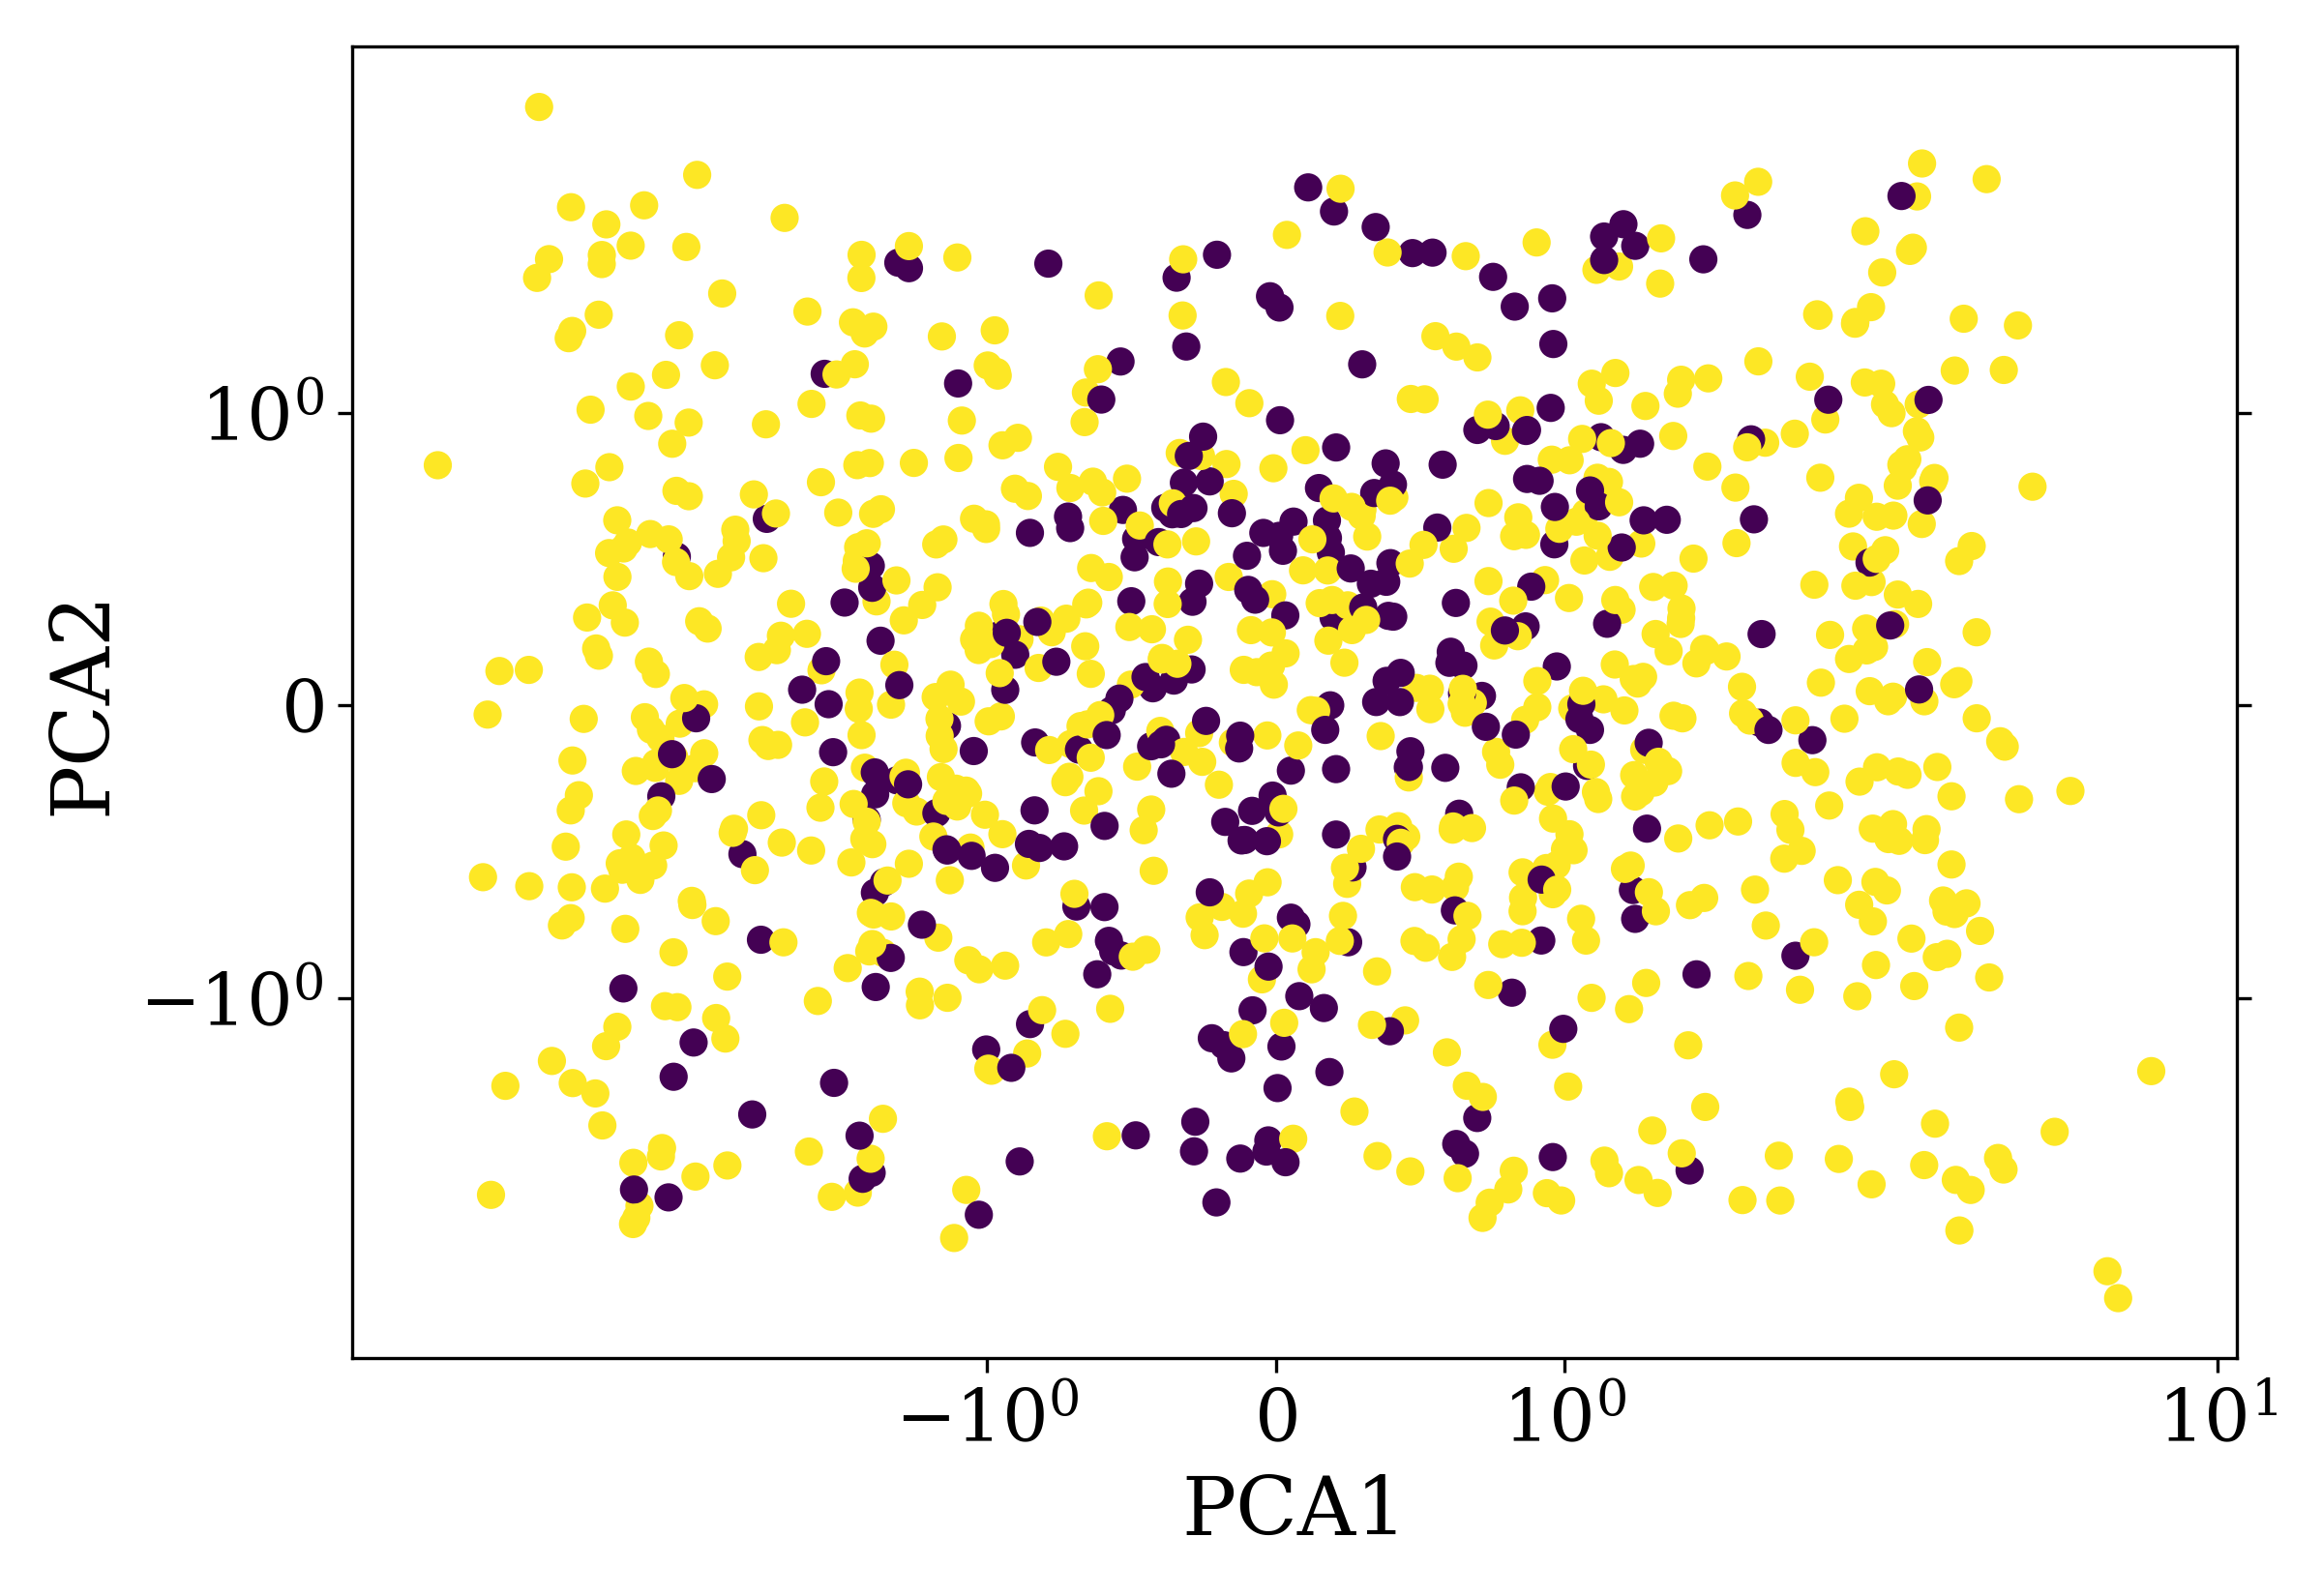
\includegraphics[width=\textwidth]{results/XGB_Diff_FIRST_True_Week_6_With_RS_True.png}
        \caption{Difference Between True Values and FIRST Values (Difference-Purple)}
        \label{fig:diff_first_real_conclusion}
    \end{subfigure}
    \hfill
    \begin{subfigure}[t]{0.495\textwidth}
        \centering
        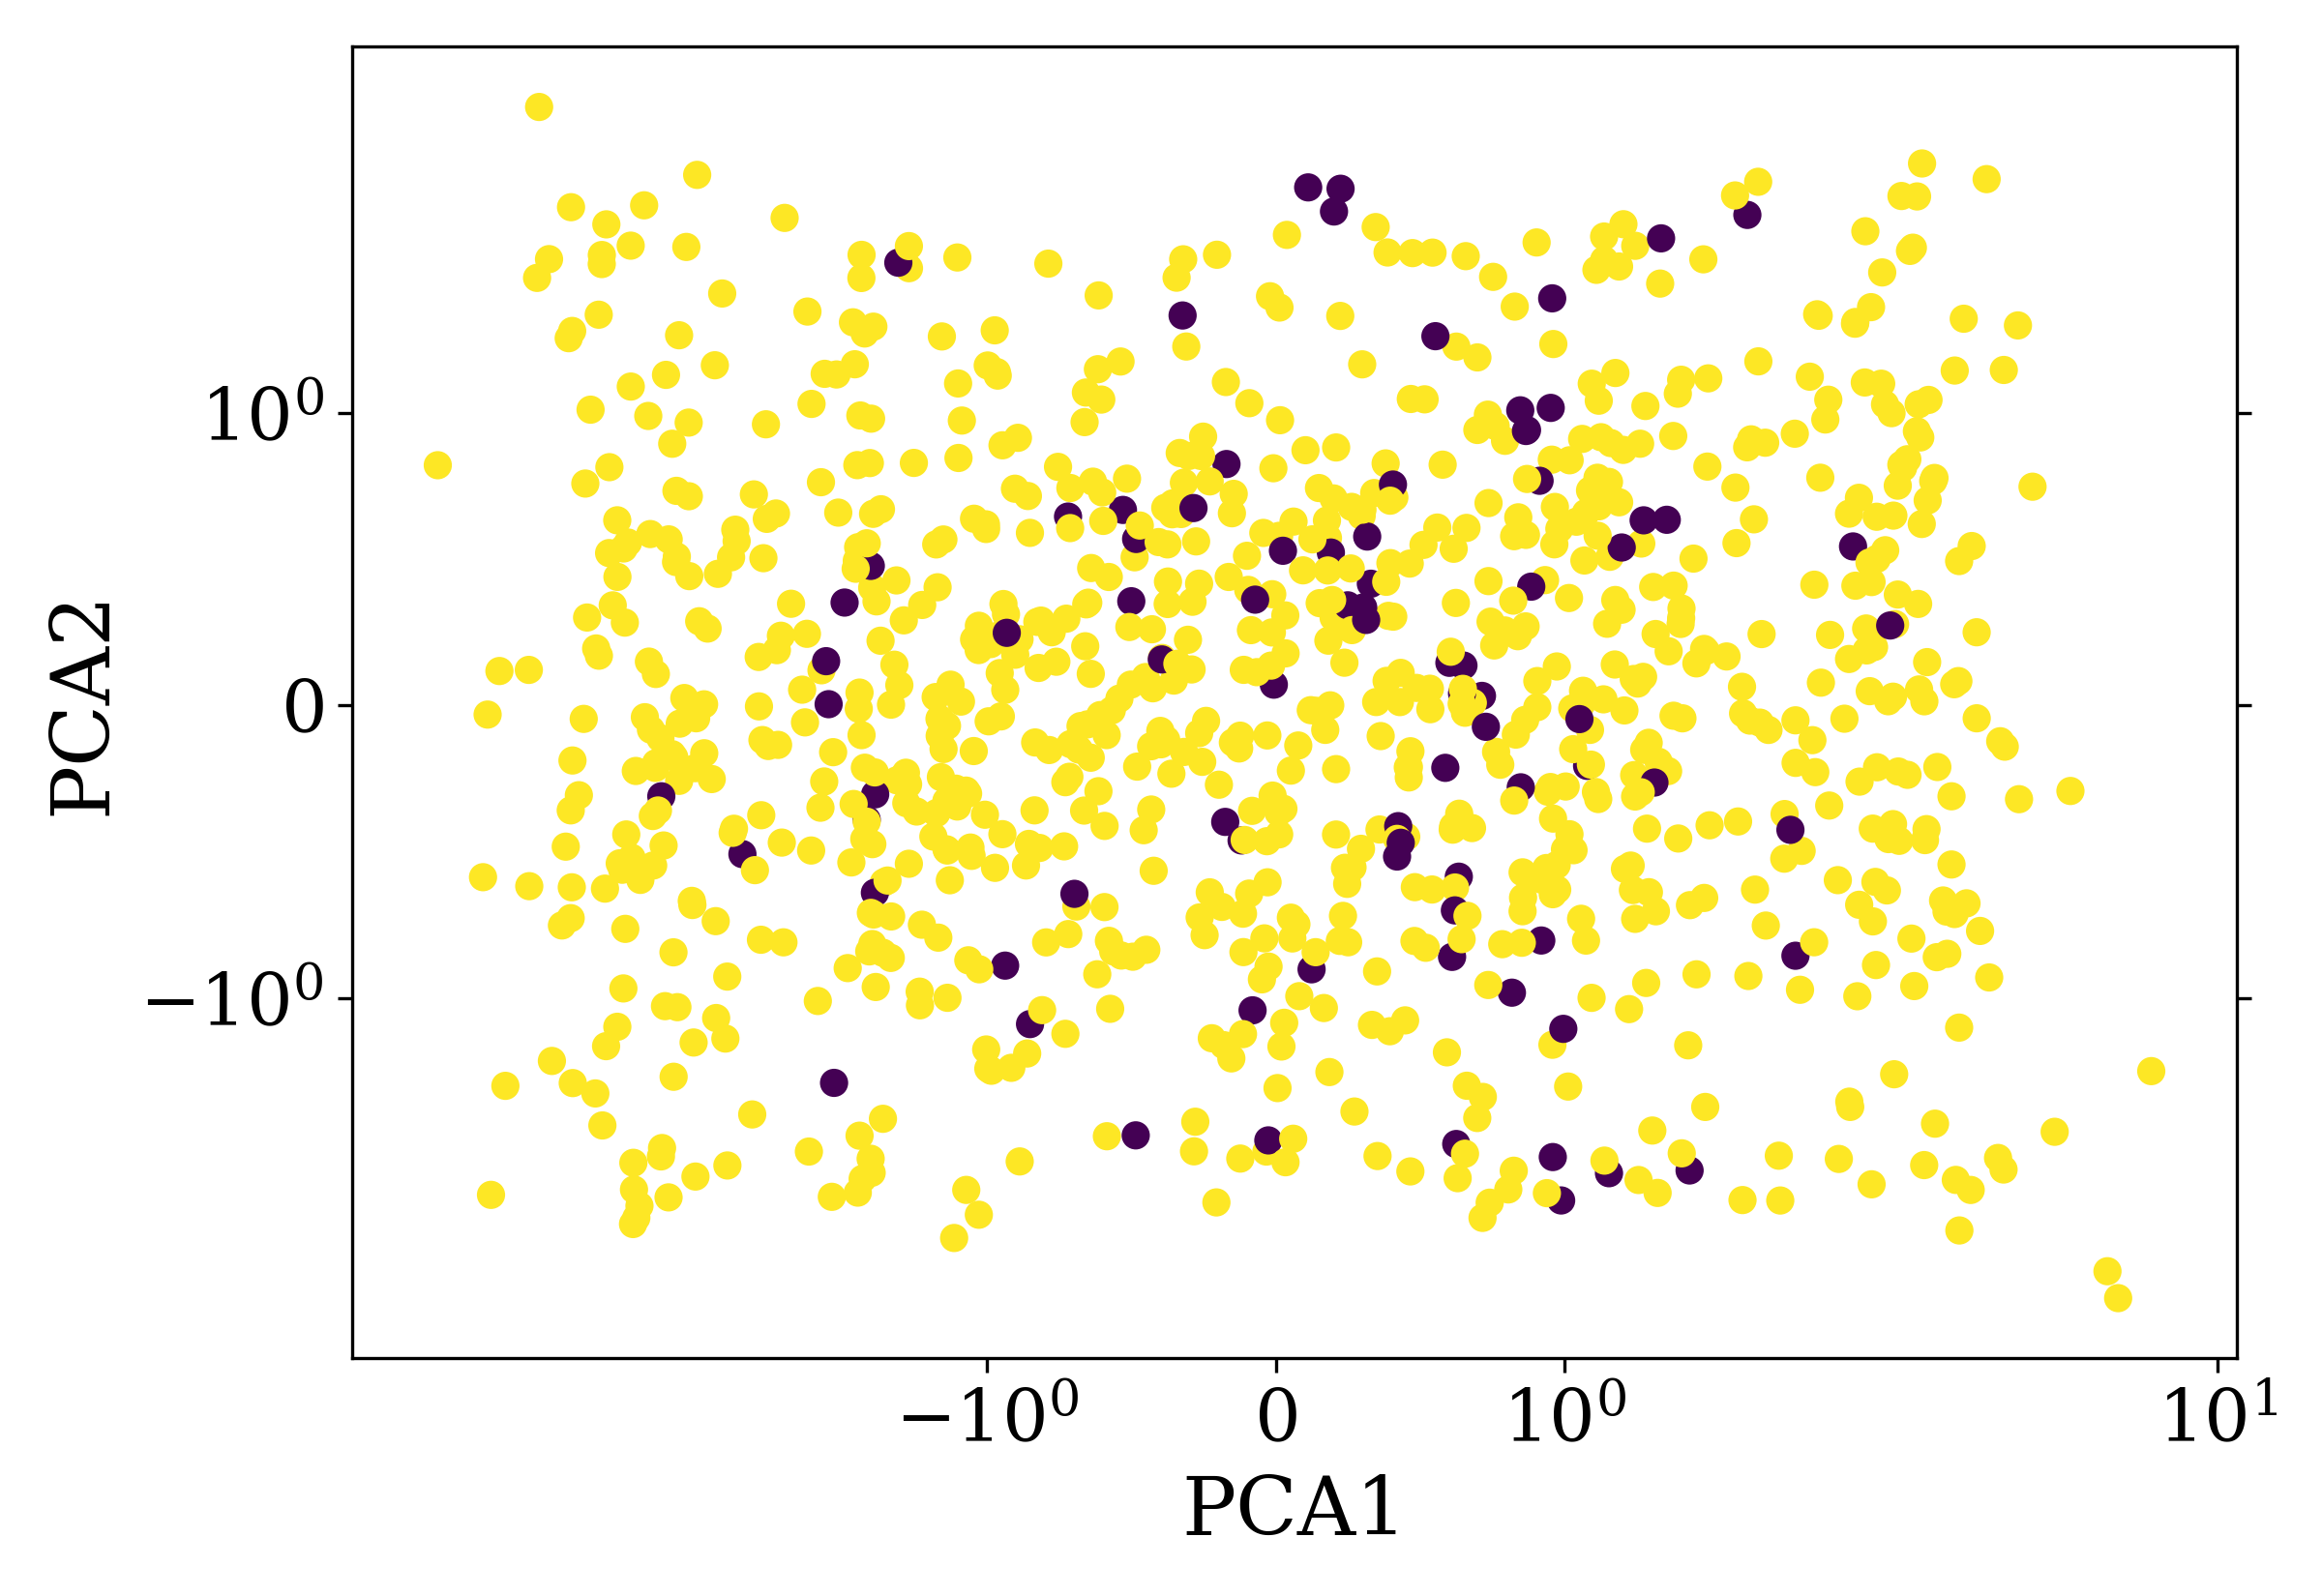
\includegraphics[width=\textwidth]{results/XGB_Diff_XGB_True_Week_6_With_RS_True.png}
        \caption{Difference Between True Values and XGB Values (Difference-Purple)}
        \label{fig:diff_xgb_first_conclusion}
    \end{subfigure}
    \caption{Difference Between First, XGB and Real For Week 6 of Testing}
    \label{fig:diff_first_xgb}
\end{figure}

\par
In the figure above, it can be easily concluded that the XGB model significantly outperforms the model FIRST uses. With an accuracy increase from 0.71900 in the FIRST model to 0.91425 in the XGB model, FIRST FRC teams will have better knowledge going into a match what their chances are if events carry out like they have previously. But, with feature importance analysis, this can be altered. With the knowledge of what makes winning teams win, teams can alter their strategies and possibly even their robots, to become more like winning teams. It is unclear what that will do to the model's ability to predict winners from losers, but adding this new dimension to strategy for FIRST FRC teams will change how the game is played.

\subsection{Reflection}
\par
This project took a long time to complete. There was no one problem that took hours to solve, but many small problems that took time to solve. One very useful module I learned of while organizing my code for this project is called "ipynb". This allows for one IPython Notebook (Jupyter Notebook) to be imported as a module. This allowed for my code to be organized into three different Jupyter Notebooks, saving space and creating less clutter. This made debugging much easier as well.

\par
The data processing and statistic calculations were not straight forward to me at first. It took some time of just sitting there, thinking about the problem to get solutions. Caching the results of the statistic calculations was a real time saver. They take about 12-15 minutes to calculate, which is awful, but is not ideal. With them cached, it takes just seconds for the data to load and be ready for use.

\par
The last thing that took time was formatting my graphs and writing the actual paper. It took a long time to get the right scales, font sizes, etc. to make the graphs look just right. Being the only visual component of this project, I knew the hard work would be worth it. For the writing of the paper, I am using \LaTeX{} on the website "Overleaf". I have never used \LaTeX{} before this project, so it was a good learning experience to learn a little bit of the language while immediately applying it to writing a paper. It took me about 5 days longer to write this than I thought because of having to learn \LaTeX, considering my \LaTeX{} file is about as many lines as my project code.

\subsection{Improvement}
\par
There are things I would like to add to this project, but I will focus here on what I did and things I could have done better. To start, I wish I used more models for the model selection phase. Limiting it to only five models covers a lot of bases of supervised learning models for binary classification, but it leaves out a lot of specialized and optimized models that could have been used. More research on this front would have been useful.

\par
Spending more time on why the XGB model's hyperparameters would not tune well would add nice closure to that. I spent quite a number of compute hours on AWS trying to optimize that model and nothing had any significant performance advantage over the default values, nothing above random error. We are talking 0.001 score difference, if that.

\par
I would have liked to evaluate the affect of the different statistics that were calculated on different model's performances. This would probably lead to some interesting results and would add importance to some statistics over others. Say, knowing that OPR is a much better statistic that CPR would be useful in analysis work and could possibly save compute time by not having CPR statistics in the data set.

\par
Lastly, I think investigating dimensionality reduction further than a quick PCA would be interesting. With the first PCA dimension having over 0.70 of the explained variance, there is quite a large amount of the data that could probably be removed with little consequence on model performance.

\clearpage
\bibliographystyle{plain}
\bibliography{references}
\end{document}
